 \documentclass[11pt]{article} 

\usepackage[round]{natbib}
\usepackage{enumitem}
\usepackage{amsmath}
\usepackage{amssymb,amsfonts,textcomp}
\usepackage{array}
\usepackage{supertabular}
\usepackage{multirow}
\usepackage{hhline}
\usepackage{graphicx}
\providecommand{\pdfshellescape}{0}
\usepackage{epstopdf}
\usepackage{color}
\usepackage[dvipsnames]{xcolor}
\usepackage{rotating}
\usepackage{appendix}
\usepackage{enumerate}
\usepackage{url}
\usepackage{booktabs}
\usepackage{floatrow} 
\usepackage{bm,array}
\usepackage{gensymb}
\usepackage{subcaption}
\usepackage{bold-extra}
\usepackage{graphicx}
\usepackage{soul}
\usepackage{eurosym}
%\usepackage[pdfborder={0 0 0}, bookmarksnumbered=true, bookmarksopenlevel=1, colorlinks=true, linkcolor=blue, urlcolor=blue, 
%citecolor=blue, hyperfootnotes=false]{hyperref}
%\usepackage[pdfborder={0 0 0}, colorlinks=true, linkcolor=blue, citecolor=blue, hyperfootnotes=false]{hyperref}
\usepackage{enumitem}
 \usepackage[labelfont=bf]{caption}
\usepackage{pdfpages}
\usepackage{amssymb}
\usepackage{latexsym}
\usepackage{graphicx}
\usepackage{xcolor}
\usepackage{lscape}
\usepackage{multirow}
\usepackage{float}
\usepackage[pdfborder={0 0 0}, bookmarksnumbered=true, bookmarksopenlevel=1, colorlinks=true, linkcolor=Blue, urlcolor=Blue, citecolor=Blue, hyperfootnotes=true]{hyperref}
\usepackage{hyperref}
\usepackage[dvipsnames]{xcolor}
\usepackage{longtable}
\usepackage{dcolumn}
\usepackage[normalem]{ulem}
\usepackage{floatrow}
\usepackage{threeparttable}
% Table float box with bottom caption, box width adjusted to content
\newfloatcommand{capbtabbox}{table}[][\FBwidth]

\usepackage{blindtext}
\usepackage{dcolumn}
\usepackage{verbatim}
\usepackage{alltt}
\usepackage{caption}
\usepackage{graphicx}
\usepackage{booktabs}
\usepackage{caption}
\usepackage[utf8]{inputenc}
\usepackage{graphbox}
\usepackage[strict]{changepage} 
\usepackage{tabularx}
\usepackage{needspace}
\interfootnotelinepenalty=10000

\newtheorem{Proposition}{Proposition}
\newtheorem{Definition}{Definition}
\newtheorem{Hypothesis}{Hypothesis}
\newtheorem{Result}{Result}

\newcommand{\jc}{\textcolor{blue}}
\newcommand{\ib}{\textcolor{red}}
\newcommand{\pb}{\textcolor{green!50!black}}
 

\renewcommand{\floatpagefraction}{.8}
\renewcommand{\topfraction}{.75}
 

 \voffset=-0.4in
 \hoffset=-0.85in
 \oddsidemargin=2.8cm
 \textheight=19.6cm
 \textwidth=15cm

 \begin{document}

 \baselineskip=14pt

 
\thispagestyle{empty} \renewcommand{\thefootnote}{\fnsymbol{footnote}}


\centerline{\Large {\bf Developmental Meritocracy}  \footnote{We thank the members of the Los Angeles Behavioral Economics Laboratory (LABEL) and the Loyola Behavioral Lab for their insights and to Chris Crabbe for his outstanding programming skills. Special thanks to Monica Vasco, Pablo Montero  and Javier Gonzalez for outstanding research assistance. We also thank the editor and referees for their constructive comments. We are grateful to the staff of Colegios Salesianos --in particular Andr\'es Corbacho, Manuel Redondo and Monica Soliss-- for their help and support in running the experiment in their schools. The study was conducted with the University of Southern California IRB approval UP-12-00528. We gratefully acknowledge the financial support of the National Science Foundation grant SES-2315770, the Spanish Ministry of Economy and Competitiveness (PID2024-156629NB-I00), the European Union's Horizon Europe Research and Innovation Programme under Grant Agreement number 101095175 and the UK Government, and the French National Research Agency (ANR) grant ANR-17-EURE-0010 (Investissements d’Avenir program).
%Address for correspondence: Isabelle Brocas, Department of Economics, University of Southern California, 3620 S.\ Vermont Ave., Los Angeles, CA 90089, USA, {\tt <brocas@usc.edu>}.
}}

\vspace*{7mm}

\noindent

\begin{tabular}{c}
\textbf{Pablo Bra\~nas-Garza} \\
\textit{Universidad Loyola Andaluc\'{i}a} \\
\textit{ }%
\end{tabular}
\hfill
\begin{tabular}{c}
\textbf{Isabelle Brocas} \\
\textit{University of Southern California} \\
\textit{IAST and CEPR}%
\end{tabular}\par  
\begin{center}
\begin{tabular}{c}
\textbf{Juan D. Carrillo} \\
\textit{University of Southern California} \\
\textit{IAST and CEPR}%
\end{tabular}
\end{center} \par \vspace*{3mm}
 
\noindent {\centerline{\underline{October 2026}}} \par \medskip

\begin{abstract}
\noindent  
We recruit 2,253 children and teenagers aged 6 to 18 in Spain to examine how young impartial observers balance merit and fairness when allocating rewards between a winner and a loser of a competition task. Using a third-party observer game, we manipulate how winners are determined---through talent, effort, or luck---and compare two reallocation methods: redistribution of tokens from winner to loser versus adding tokens to both. Participants allocate less to the loser when equalization requires taking tokens from the winner. Under addition, the estimated age profile rises through early adolescence and then tapers off, especially for final allocations; under redistribution, the corresponding profile is comparatively flat.
Pooled estimates also indicate lower transfers to the loser when the winner is selected by talent rather than luck, while estimates for effort relative to luck are small or imprecise. Finally, allocation decisions are related to gender, personality traits, and the observer's capacity for empathy, with male participants exhibiting more meritocratic allocation patterns.
Overall, our results show that the development of redistributive preferences is sensitive to the institutional mechanism through which redistribution is implemented.
\end{abstract}   

\noindent \underline{Keywords}: lab-in-the-field experiment, developmental decision making, third-party observer, inequality.

\noindent \underline{JEL Classification}: C93, D63.



\newpage


\setcounter{page}{1} \renewcommand{\thefootnote}{\arabic{footnote}} %
\setcounter{footnote}{0}

 \section{Introduction}
Redistributive preferences is a central issue in policy debates.
An individual's tolerance for inequality depends on four key factors: who benefits or suffers from inequality, the perceived cause of inequality, the method of redistribution, and the attributes of the individual making the judgment. Also, redistributive preferences evolve over time, raising important questions about the interaction between innate dispositions and life experiences, particularly during childhood and adolescence.

This study focuses on \emph{normative redistributive preferences}, examining how impartial observers decide to allocate resources between a wealthier and a poorer individual. We investigate how redistributive judgments change with age, tracing the development of these preferences from childhood to adulthood and linking them to affective development and life experiences. Additionally, we explore how attitudes toward inequality vary depending on its source and how different redistribution mechanisms influence these preferences.

Redistributive preferences in adults have been extensively studied in the experimental literature.\footnote{Examples include \citet{charness2002understanding} on the nature of social preferences, \citet{cappelen2013just} on fairness views related to risk-taking, and \citet{andreoni2020fair} on ex-ante vs.\ ex-post fairness, among others.} Existing work, particularly through dictator and ultimatum games, has documented behavioral tendencies such as altruism, egalitarianism, envy, and inequity aversion when individuals have a personal stake in redistribution \citep{engel2011dictator, oosterbeek2004cultural, fehr2006economics}. These studies also demonstrate that individuals are sensitive to the framing of allocation decisions \citep{list2007interpretation} as well as to the origin of inequality \citep{fong2001social, konow2000fair}. However, normative preferences---those expressed by third-party observers---have received comparatively less attention. An exception is the work of the FAIR group, which has examined how impartial adult observers allocate resources based on the source of inequality. \citet{cappelen2019meritocratic} find that observers are more likely to favor equitable distributions when disparities result from luck rather than productivity. \citet{almaas2020cutthroat} show that while many Americans consider both luck- and productivity-based inequalities fair, Norwegians are more likely to reject them as unfair. These findings highlight the complexity of redistributive preferences among adults.

Our allocation-method comparison is related to, but distinct from, the give-versus-take manipulation in \citet{list2007interpretation}. List studies self-interested adult dictators and expands their action set to include taking from the recipient. We instead study impartial observers who allocate rewards between two other participants, and we hold the feasible set of final allocations fixed across \emph{redistribution} and \emph{addition}. Thus, our comparison asks whether the procedure used to implement the same final allocations affects normative judgments, and how this sensitivity develops from childhood through adolescence.

 
Research on the development of social preferences from childhood to adulthood has focused mainly on dictator games. 
A pioneering study by \citet{Fehr2008} examined the choices of children aged 3 to 8 in three binary dictator games and found that preferences for equality increase with age. \citet{fehr2013development} extended the analysis to children aged 8 to 17 and demonstrated a growing preference for (costless) egalitarianism across the sample.\footnote{\citet{branas2024} replicates \citet{Fehr2008}'s experiment with 2,525 Spanish teenagers and finds that egalitarianism increases across the entire sample, while altruism drops sharply. \citet{brocas2020development} examine children aged 7 to 16 playing a dictator game where they can manipulate information to hide undesired consequences, and find that  20\% to 30\% do so.}
In \citet{almaas2010fairness}, children aged 10 to 18 first completed a production task in which earnings depended on both effort and randomly assigned luck, and then decided how to distribute these earnings between themselves and a partner. The authors show that the prevalence of strict egalitarian views declines with age, whereas meritocratic views become increasingly prevalent. These studies suggest that context effects (triggering either selfish or deontological concerns) may lead to different behavioral patterns.




Distributive preferences by third party observers in a developmental setting have been rarely studied experimentally. \citet{angerer2017} and  \citet{barron2023discrimination} are two exceptions that focus on in-group favoritism based on language and nationality, respectively (see \citet{sutter2019survey}'s survey).  

Studying third-party observers is important not only because real-world redistribution decisions in policymaking, judicial settings, and workplaces are often made by such actors, but also because it isolates decision-makers who have no material stake in the outcome, thereby removing self-interest from the equation. This allows for a clean understanding of how individuals of different ages justify inequality without the confounding influence of personal implication. Moreover, a systematic examination of these preferences under different conditions can provide insights into why people respond differently to inequality across contexts and, ultimately, how institutional design can influence redistributive outcomes. 
Overall, as we develop below, in this paper we systematically analyze redistributive preferences by impartial observers at different ages, under different redistributive mechanism, and for different sources of inequality. We also link behavior to experience, gender, personality traits and emotional intelligence.


For our study, we recruited a large population of 2,253 children and teenagers aged 6 to 18 years old from low- to middle-income families in Spain. Participants acted as impartial observers, deciding how to allocate resources between two players competing in a task. The study incorporates three competition tasks, each aimed at capturing different sources for inequality: \emph{luck}, \emph{effort} and (a novel) \emph{talent} task. In each case, the winner receives a higher payoff than the loser. We also implement two reallocation methods. First, a take-from-the-rich method (as in \citet{cappelen2019meritocratic} and \citet{almaas2020cutthroat}), where the observer can \emph{redistribute} payoffs from the winner to the loser. Second, a novel top-up method, called \emph{addition}, where the observer decides how to allocate additional payoffs between the winner and the loser. Importantly, the feasible set of final allocations is identical in both cases. 


Impartial observers also participate as competitors. Participants first choose an allocation as outside observers, then engage in a competitive task, and finally make a second allocation decision, with the option to revise their initial choice. This sequence allows us to examine how allocations change after participants experience the task. Because all participants are also invited to reconsider their initial choice, the design does not separately identify the effect of experience from reflection or repeated measurement. Finally, we introduce two novel child-friendly non-cognitive tasks: an affective theory-of-mind test and a pictorial personality questionnaire.

We obtain the following insights. First, participants allocate less to the loser under redistribution than under addition, consistent with a reluctance to take rewards from the winner. Second, the estimated age trajectory is more pronounced under addition, where transfers to the loser rise through middle school and decline afterwards in the final allocation; the corresponding profile under redistribution is comparatively flat. Third, pooled estimates indicate a talent--luck difference, whereas effort--luck estimates are generally small or imprecise. Fourth, revisions are systematically associated with participants' perceptions of task difficulty and own performance: individuals who found the competition easy and believed they performed well are more inclined to increase the reward of the winner. These patterns are also related to gender, personality traits, and affective processes. In particular, more empathic and agreeable individuals favor ex-post fairness, whereas more conscientious individuals, as well as male participants, display a stronger tendency toward meritocratic allocations.



The results underscore the complexity of redistributive preferences and highlight the interplay between cognitive development, experience, and personality traits in shaping attitudes toward inequality. The distinction between redistribution and addition reveals that procedural sensitivity is already present among children and adolescents. Our estimates also suggest that the perceived basis of success matters: the talent--luck contrast is clearest in pooled final-allocation specifications, while the evidence for effort is less precise. Finally, post-task revisions are correlated with participants' own experience and perceptions, although our design cannot separate this channel from reconsideration of the initial choice.

More generally, our findings uncover developmental patterns that diverge from those found in dictator game settings, highlighting the value of disentangling between redistribution by an observer and redistribution by an affected party. Since these dependencies evolve with age, they highlight the dynamic nature of fairness preferences and underscore the need to consider both developmental and contextual factors when examining attitudes toward redistribution.  
 
 
\enlargethispage{2\baselineskip}
The paper is organized as follows. In section \ref{sec-design}, we present the experimental design. Section \ref{sec-model} develops a formal model. In section \ref{sec-results}, we discuss the main results, including the effect on choice of age, origin of inequality and allocation mechanism. We also study the influence of personality and affective theory of mind on allocation decisions. In section \ref{sec-conclusion}, we present some concluding remarks. 
 
\section{Experimental design and procedures \label{sec-design}} 

We recruited children and adolescents to study the decision of an impartial observer who allocates rewards between two competitors. We follow the guidelines presented in \citet{brocas2019survey} to address the methodological challenges that arise in studies with young participants. \par \medskip

\emph{Experiment}. The experiment consists of two games programmed in `oTree' \citep{chen2016otree}. This study focuses on the first game, the third-party dictator. After a short break, participants played a two-person game with incomplete information, which we analyze in a separate paper \citep{alfonso2023development}.\footnote{The two games are distinct enough that we are not worried about cross-contamination. However, as a precautionary measure, we always conducted the two games in the same order, anonymously re-matching subjects between the two games, and did not disclose any result until the conclusion of the second game.} \par \medskip
  
 
\emph{Timing}. We first informed participants that they all would play an ``observer task" followed by a ``competition task". We emphasized that if a participant acted as the observer for two competitors, neither of those competitors would serve as their observer. In the observer task, participants allocated tokens between a future winner and a future loser of the competition task. In the competition task, they competed in pairs for a prize. We also informed them that feedback would be provided only at the end of the experiment. After the competition task, they were given the option to modify their decision in the observer task,
with clear emphasis that no further modifications would be possible afterwards. These tasks were followed by the second game, an affective theory-of-mind task, and a Big 5 personality questionnaire (both described at the end of this section). The instructions were read aloud to participants while the corresponding PowerPoint slides were projected on a screen. The instructions for the observer and competition tasks are provided in Appendix A1. \par \medskip
 
  
\emph{Observer task}. The impartial observer game used a visually intuitive interface (see Figure \ref{fig-task}). Participants allocated tokens by dragging them between the winner (depicted by a trophy) and the loser (depicted by a crossed-out trophy). They could adjust the allocation freely until pressing {\sc ok} to finalize their decision. 

We explored two different environments for allocating tokens. First, a \emph{redistribution\/} method, characterized by an initial allocation of (6,2) between the winner and the loser, with the observer able to redistribute 0, 1, or 2 tokens from the winner to the loser. This design is similar to the existing literature \citep{cappelen2019meritocratic, almaas2020cutthroat}.
The second is an \emph{addition} design, where observers do not take tokens from the winner. Instead, the initial allocation is (3,1), and 4 additional tokens must be distributed between the two competitors, with at least one token allocated to each. Figures \ref{fig-screen-split-6-2} and \ref{fig-screen-split} show screenshots of both environments. 
Note that the three possible final allocations are identical in both environments: a ``meritocratic" split (6,2) that maximizes the difference between winner and loser (while ensuring both receive a positive amount), a ``compensatory" split (4,4) that equalizes final payoffs regardless of performance, and an ``equitable" split (5,3) that provides an intermediate option. However, we expect that the framing of the allocation method, take-from-the-rich (\emph{redistribution}) vs.\ top-up (\emph{addition\/}), may trigger different behavioral responses. \par \medskip

\begin{figure}[htpb]
\noindent \hspace*{-5mm}
    \begin{subfigure}[b][][t]{0.44\textwidth}
   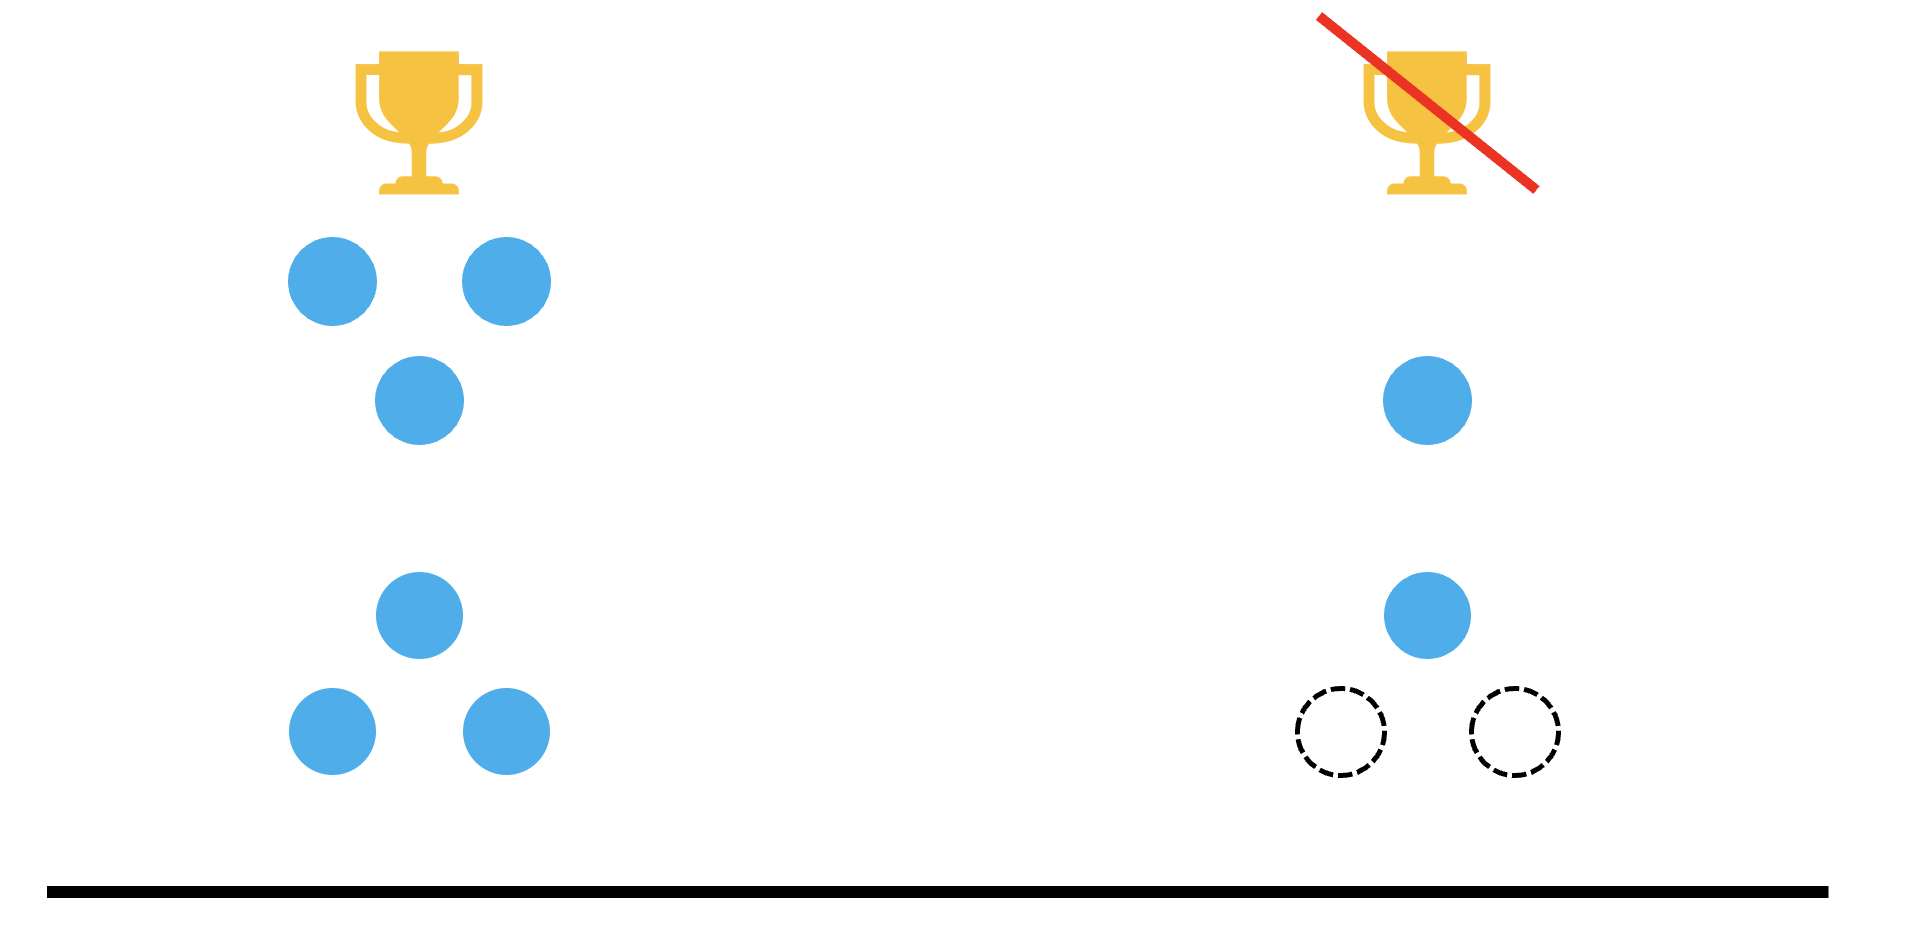
\includegraphics[height=1.35in]{Figs/screen-split-62.png} \vspace*{0.1mm}
      \caption{\emph{Redistribution}: 0, 1, or 2 tokens can be taken from winner and transferred to loser\label{fig-screen-split-6-2}}
    \end{subfigure}
\hspace*{4mm}
 \begin{subfigure}[b][][b]{0.54\textwidth}
      \centering
   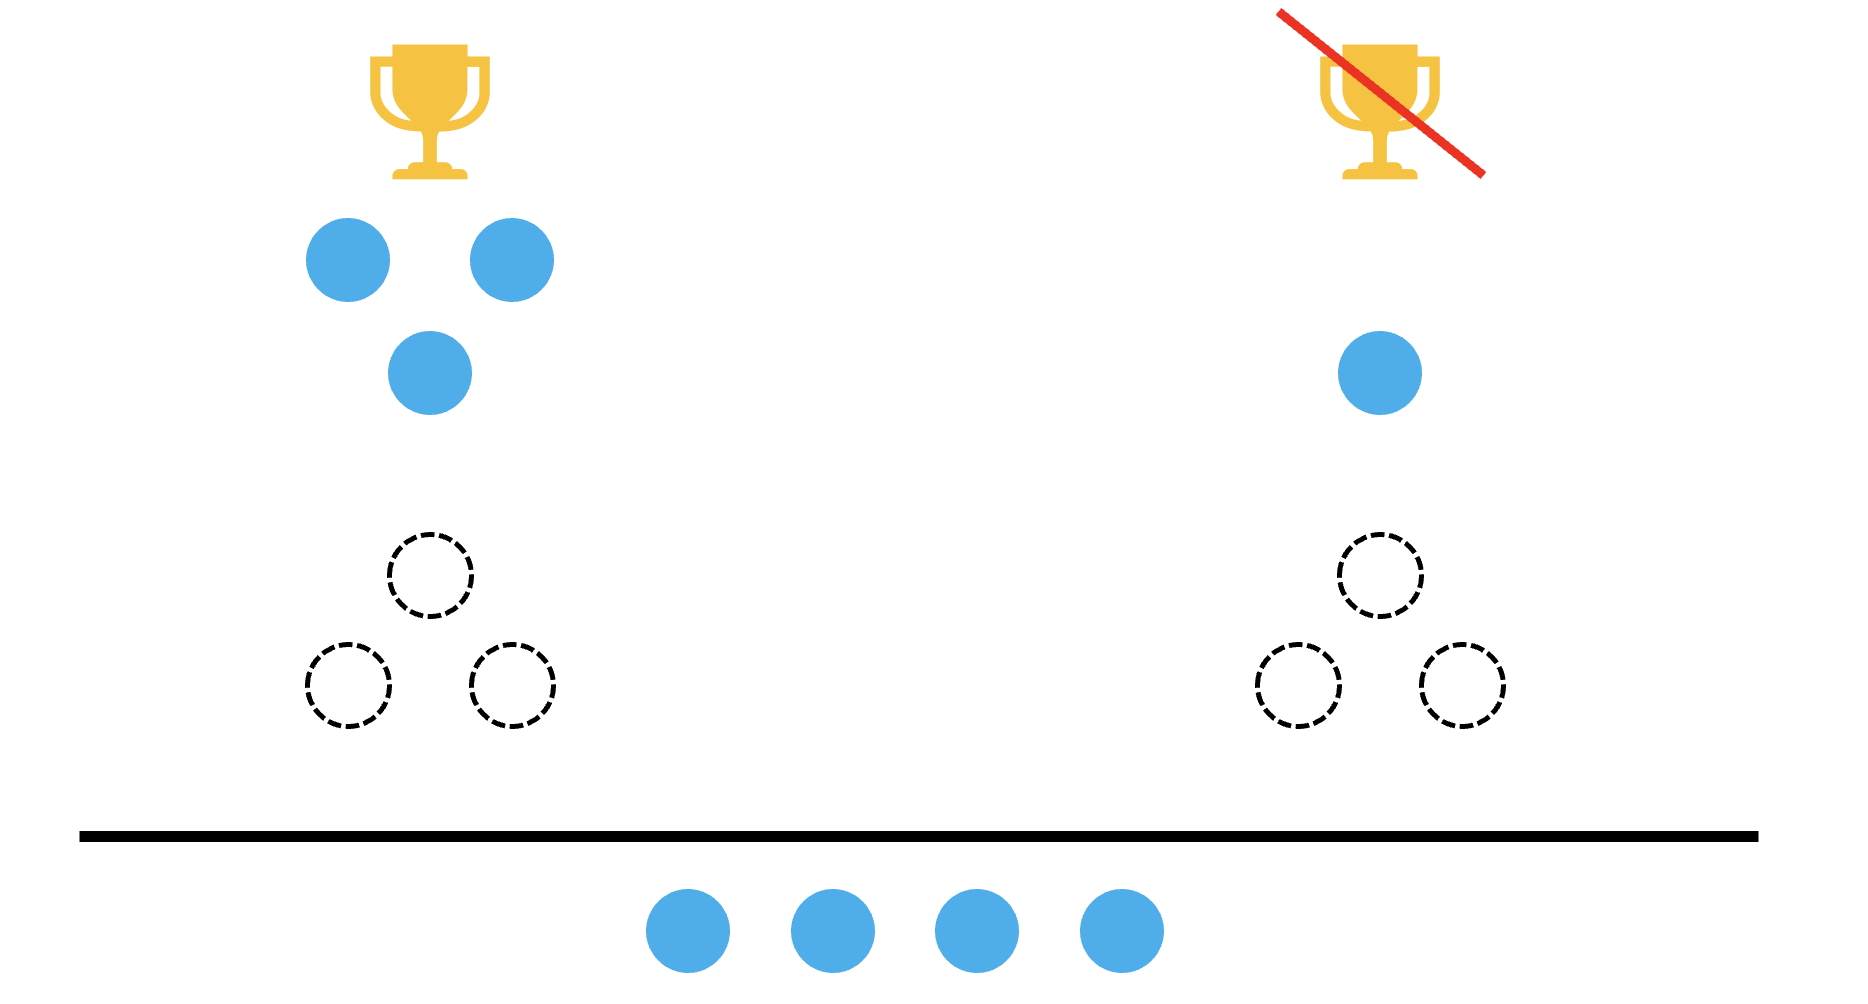
\includegraphics[height=1.5in]{Figs/screen-split-31.png} 
      \caption{\emph{Addition}: 4 tokens (bottom) must be allocated between winner and loser (with at least one for each)\label{fig-screen-split}
      }
    \end{subfigure}
\caption{Screenshots of the observer task: redistribution (left) v.\ addition (right)} \label{fig-task}
\end{figure} 


\emph{Competition task}. We explored three procedures for determining the winner of the competition, which encompass the three fundamental factors of performance in conventional economic models: \emph{effort},  \emph{talent\/} and \emph{luck}.\footnote{Canonical models of performance are typically summarized by $y=f(e,\theta)+\eta$, where $y=$ performance, $e=$ effort, $\theta=$ ability, and $\eta$ is a stochastic component.}

In the \emph{effort\/} task, participants were randomly and anonymously paired to compete in an effort-intensive activity requiring patience and concentration. Following \citet{gill2012structural}, we employed a slider task. Each participants faced 39 non-aligned sliders, each starting at a random position between 0 and 100 (but never 50). The participant who successfully positioned the most sliders at exactly 50 within 90 seconds was the winner.\footnote{In case of a tie, the participant who reached that number of sliders first was the winner. Participants were never informed of the exact performance difference between winner and loser.} Prior to the competition, participants completed a short practice round where they adjusted three sliders to 50.  \autoref{fig-screen-slider} provides a screenshot of the effort competition task, showing four sliders already set at 50 and a timer indicating 31 seconds remaining.

In the \emph{talent\/} task, participants answered a series of 8 to 12 age- and culture-appropriate multiple-choice general knowledge questions, covering topics such as mathematics, biology, history, sports, and entertainment. Participants had, depending on age, 12 to 18 seconds to select one of four possible answers. The participant who answered the most questions correctly was declared the winner. Before the competition, participants completed a practice question to familiarize themselves with the format. \autoref{fig-screen-trivia} displays a screenshot of the talent competition task (translated from the original Spanish version). 

In the \emph{luck\/} task, participants were simply informed that the computer would randomly select a winner and a loser from each pair, with equal probability. 

\begin{figure}[htpb]
    \centering
\hspace*{-8mm}   
\noindent \begin{subfigure}[b]{0.47\textwidth}
   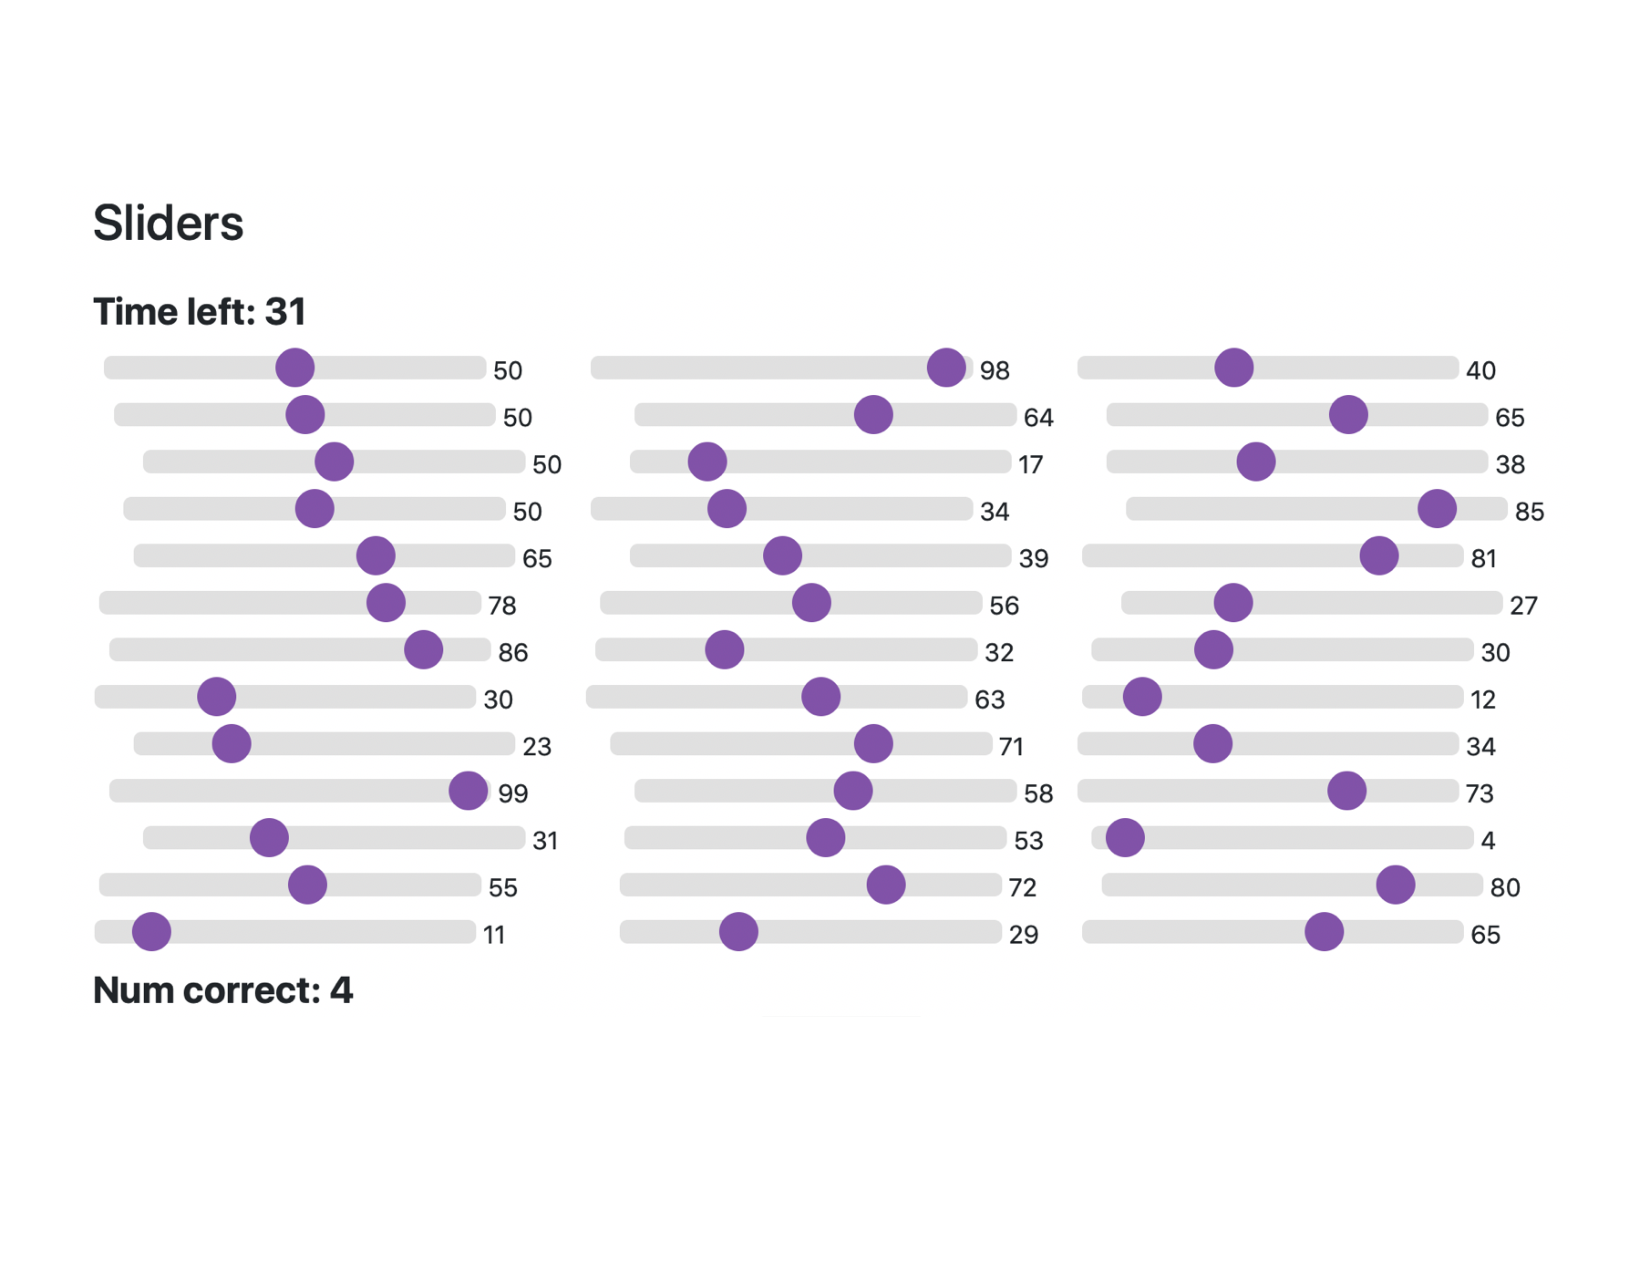
\includegraphics[height=1.35in]{Figs/screen-sliders.pdf} 
      \caption{\emph{Effort}: participants had 90 seconds to position as many sliders as possible at 50\label{fig-screen-slider}
      }
    \end{subfigure}
 \hspace*{4mm}   \begin{subfigure}[b]{0.52\textwidth}
      \centering
   
\includegraphics[height=1.1in]{Figs/screen-trivia.pdf} 
      \caption{\emph{Talent}: participants answered age-appropriate, multiple choice general knowledge questions\label{fig-screen-trivia}
      }
    \end{subfigure}
\caption{Screenshots of the competition task: effort (left) v.\ talent (right) } \label{fig-treatments}
\end{figure} 
 
Overall, the experiment consists of six variants, following a $3\times 2 $ between-subject design: three conditions for determining the winner (\emph{effort}, \emph{talent}, and \emph{luck}) and two treatments for the allocation of tokens (\emph{addition\/} and \emph{redistribution}). Crucially, the design varies these two dimensions orthogonally. This one-factor-at-a-time structure allows us to attribute differences in outcomes to each dimension without confounding. \par \medskip

  
\emph{Population}.
We enrolled an unusually large sample for a lab-in-the-field experiment: 2,253 school-age students from low- to middle-income families, spanning grades 1 to 12 in the Spanish equivalent of the US education system. Participants came from four schools located in different cities across the southwestern region of Spain. All schools belong to Salesianos, a private network of Catholic schools funded by the Spanish government.\footnote{The Salesianos educational network has 59 schools in Spain serving almost 40,000 students (see {\tt https://www.salesianos.es/escuelas}).} 
The experiment was integrated into the school’s academic curriculum, with our Institutional Review Board (IRB) approving an opt-out procedure. Notably, no students opted out, eliminating the risk of selection bias. The only students who did not participate were those absent on the day of the experiment (5.7\%). Treatment assignment was implemented at the class -- or half-class -- level (rather than at the individual level), while pairings within each session were anonymous and randomly determined. This approach reflects the realities of school-based implementation: students are scheduled and tested one class at a time, making class-level assignment the feasible and standard unit of randomization. Moreover, individual-level assignment is difficult to communicate to young children and could introduce confusion or demand effects.
\autoref{table-population2} summarizes the distribution of the 2,253 participants by grade, type of competition, and token allocation method. Of the 2,299 students who took part, 41 selected a gender category other than male or female and 5 did not report gender; these 46 observations are excluded from the analyses reported here, which use the binary Male control. Some further observations are excluded depending on the analysis: the regressions on age exclude 10 participants aged 225 months or more; in the \emph{addition} environment, the software did not record the initial choice of 2 participants and the final choice of 14; and 8 participants have no DeRMET answers, 25 have incomplete P-Big 5 answers, and the task-perception questions were not recorded in two sessions (46 participants).

\begin{table}[htpb]
\small
\setlength{\tabcolsep}{.62\tabcolsep}
\begin{tabular}{lccccccccccccccc}  
%& & \multicolumn{12}{c}{\textsc{spain}} \\
Grade  			& & 1 & 2 & 3 & 4 & 5 & 6 & 7 & 8 & 9 & 10 & 11 & 12 & & Total \\ [-2.4ex] \\  \midrule \\ [-5.0ex] \\
% Age 			& & 8-9 & 9-10& 10-11 & 11-12 & 12-13& 13-14& 14-15 & 15-16 & 16-17& 17-18 \\ 
addition / effort 			& & 28  & 30  & 32 & 31  & 20  & 24  & 54  & 27  & 23 & 50 & 23 & 0 & & 342 \\ 
addition / talent 	& & 22 & 26  & 25  & 23  & 52  & 47  & 30  & 29  & 51 & 25 & 31 & 24 & & 385  \\ 
addition / luck 		& & 22  & 22  & 22 & 24  & 24  & 50   & 26  & 80  & 54 & 46& 29 & 45 & & 444\\   [-2.1ex] \\
redistribution / effort 	& & 19  & 28  & 23 & 25  & 45  & 22  & 54  & 52  & 31 & 28 & 23 & 34 & & 384 \\  
redistribution / talent 	& & 32  & 8  & 22 & 21  & 49  & 43  & 27  & 26  & 31 & 25 & 29 & 20 & & 333 \\  
redistribution / luck 	& & 15  & 22  & 33  & 33  & 25  & 26  & 62  & 29  & 28 & 43 &23 & 26 & & 365  \\    \midrule
Total & & 138 & 136 & 157 & 157 & 215 & 212 & 253 & 243 & 218 & 217 & 158 & 149 & & 2253 \\  
\end{tabular} 
\centering\caption{Number of participants by grade, treatment, and condition} \label{table-population2}
\end{table}

\emph{Payments}.
We identified a payment method that was uniform across all ages and highly valued by participants. All four schools in this sample have integrated cafeterias where students can purchase drinks, food and snacks at discounted prices. The cafeteria is very popular and widely accessed during recess and lunch, with items such as sandwiches and soft drinks highly and equally valued by students of all ages. To incentivize participants, we created our own currency, which could be spent on any item in the cafeteria. The currency had no expiration date, although most participants spent their endowments within a week. The exchange rate was 1 token = 1\euro. \par \medskip


\emph{Developmental Read the Mind in the Eyes Task (DeRMET)}. Next, we introduced participants to a novel, incentivized affective theory-of-mind task to examine the link between social preferences and the ability to empathize with others. This task builds on the original ``Read the Mind in the Eyes Task" (RMET), a psychological assessment developed by  \citet{baron1997another} to measure individuals' ability to attribute complex mental and emotional states to others. In that task, participants view images of a person’s eyes and select the adjective that best describes the emotion being conveyed. The RMET was originally designed for adults, with emotions that reflect subtle nuances and are described using sophisticated language. The standard adaptation of the RMET to children, which consists in presenting a subset of the original images \citep{baron2001studies}, has been shown to not perform very well in young populations \citep{van2017comparison}.
We therefore created an alternative RMET task, called DeRMET (Developmental RMET), specifically for children and adolescents. The task was tested, registered with the Open Science Framework (OSF), pre-validated with 43 teenagers and adults, and validated with the 2,253 observations collected in this experiment (see Appendix B7 for details). It is a unique tool for researchers interested in studying the development of emotional intelligence and its association to decision-making processes. 
 
 Our adaptation features 16 images capturing the expressive eyes of a 12 years-old preteen who conveys 16 fundamental emotions, all described in simple language. For each image, we provide four possible answers, one of which most accurately represents the intended emotion. This modified version of the task offers three advantages for our population. First, sourcing all images from a single individual ensured greater consistency. Second, using a child as the model made the images more relatable for children and adolescents. Finally, focusing on simpler emotions and using straightforward language made the task appropriate for all ages, including the youngest participants.\footnote{Other authors have developed variations of the RMET task, or emotional intelligence tasks based on facial expressions (see e.g., \citet{mattek2021100, pahnke2020reading}). To our knowledge, none are designed to study the developmental trajectory of affective theory-of-mind.} \autoref{dermet} shows one example image along with the four answer choices presented to participants (65\% selected the correct answer, ``sad”).\footnote{An answer is labeled ``correct” if it is \emph{both\/} the emotion the preteen intended to convey in the image and the one chosen by the majority of participants. The two criteria coincide for all 16 images.} Detailed instructions, including the full set of images, possible answers, correct responses, and the percentage of participants who answered each one correctly, are provided in Appendix A2.
  
 \begin{figure}[htpb]
    \centering
%\hspace*{-2mm}   
\noindent \begin{subfigure}[b]{0.52\textwidth}
   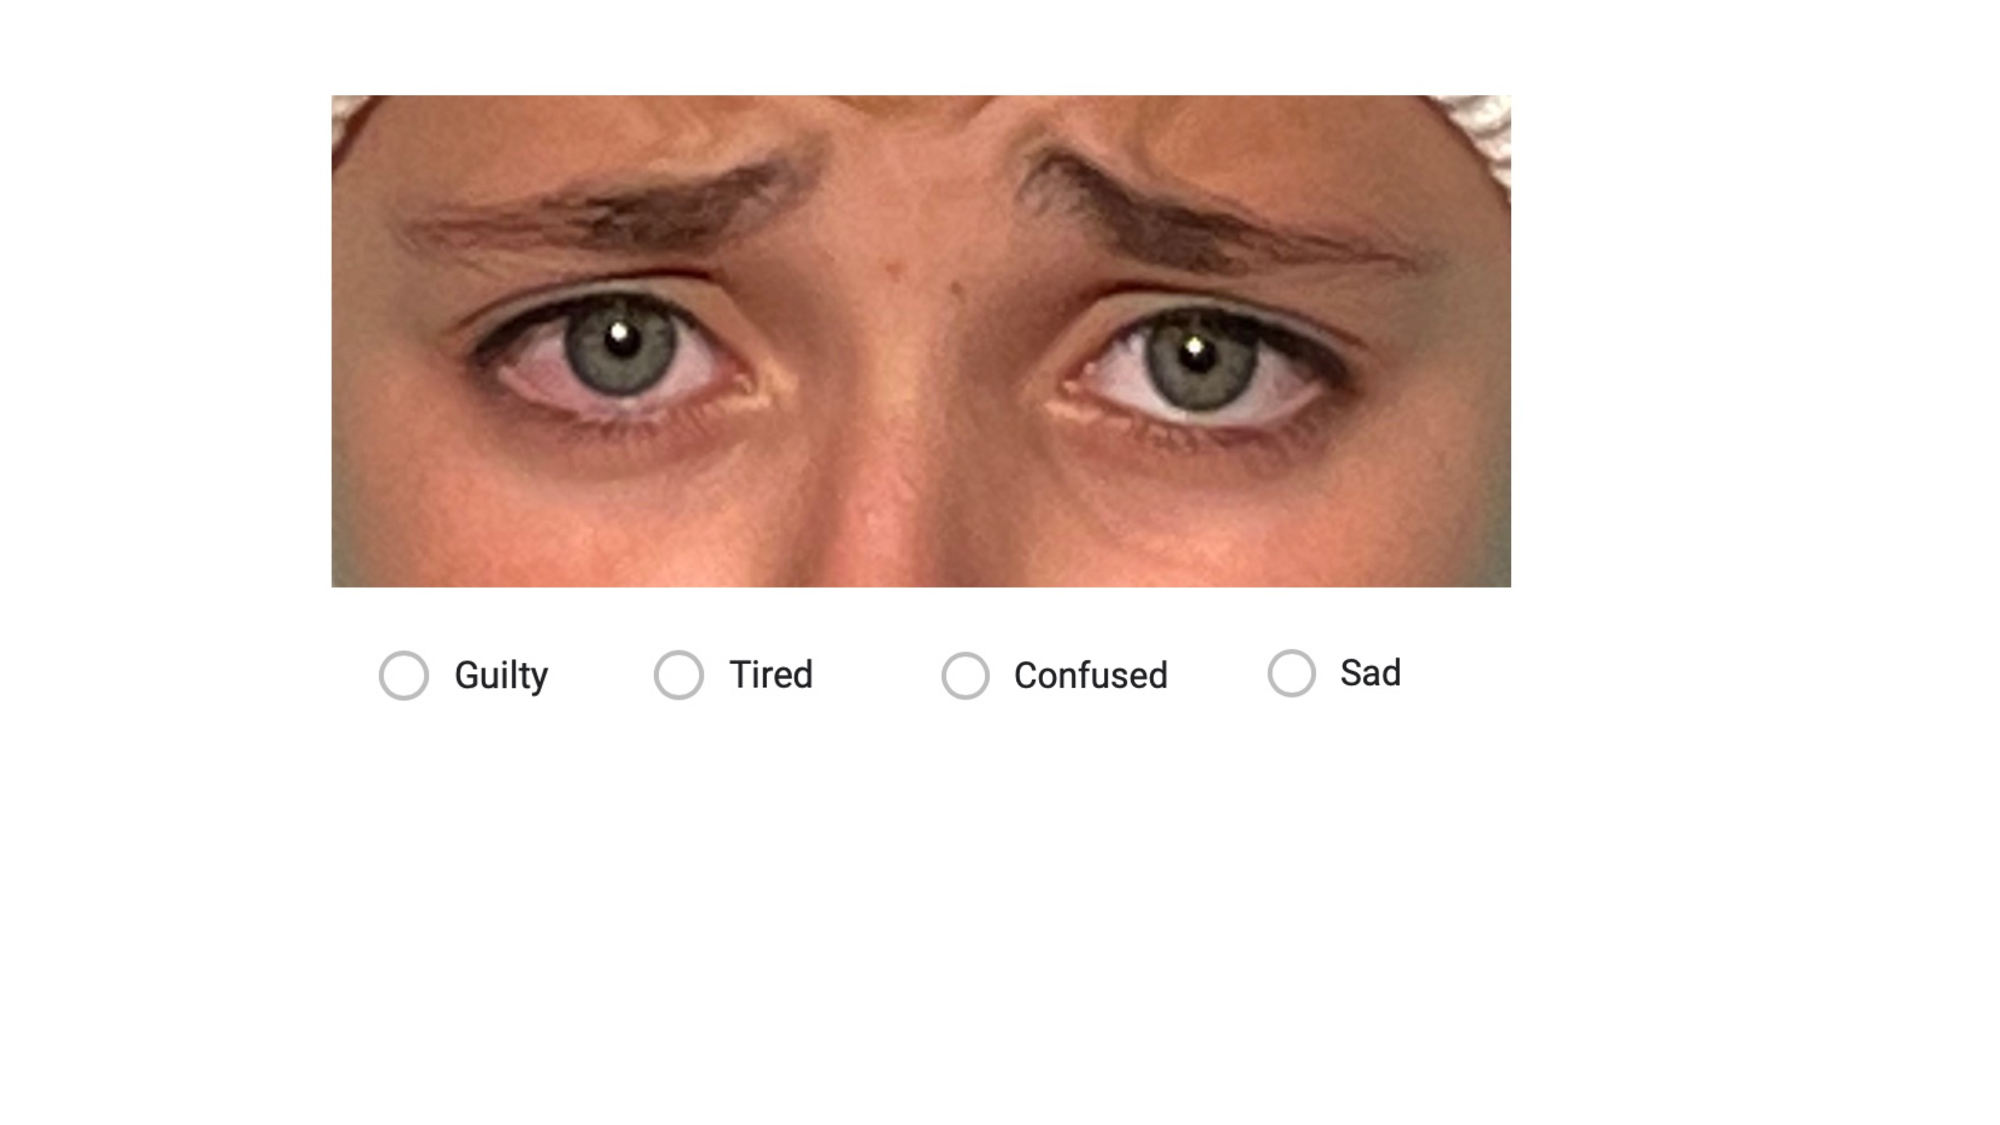
\includegraphics[height=1.35in]{Figs/aTOM.pdf}  
      \caption{Developmental RMET} \label{dermet}
    \end{subfigure}
 \hspace*{2mm}   \begin{subfigure}[b]{0.45\textwidth}
      \centering
   \includegraphics[height=2.0in]{Figs/personality4.png}  
   \caption{Pictorial Big Five (neuroticism trait)} \label{p-big5}         
   \end{subfigure}
\caption{Examples of DeRMET and P-Big 5} \label{noncognitive}
\end{figure} 
\medskip


\emph{Pictorial Big Five (P-Big 5)}. Next, we performed a novel version of the Big Five questionnaire, to study the joint evolution of personality and social preferences. A typical objective in psychology is to categorize individuals across the ``Big 5" personality traits: openness, conscientiousness, extraversion, agreeableness, and neuroticism \citep{fiske1949consistency, %norman19672800, 
mccrae1987validation, goldberg1993structure}. Studies have employed a wide array of verbal questionnaires to examine those traits and how they relate to behavior and life outcomes. These verbal questionnaires can pose significant challenges for young participants, particularly when subtle emotional states are involved. In studies with children, assessments often rely on variants completed by parents or caregivers. However, for the developmental trajectory of personality, it is crucial to employ a single assessment tool to ensure meaningful comparisons across various age groups.

To address these challenges and ensure consistent testing across individuals aged 6 to 18, we again developed a novel, child-friendly version of the Big 5 questionnaire, which we call the Pictorial Big 5 (P-Big 5). In this version, each trait is represented by a set of images illustrating opposite ends of the trait spectrum. Participants are shown a 5-point Likert scale and asked to select the option that best describes how they perceive themselves. The task was again tested, registered with OSF and pre-validated with 40 teenagers and adults who completed our P-Big 5 and a 25-question variant of the Five-Factor Model created for adolescents \citep{rogers2018development}. We then validated the task with the 2,280 observations collected in this experiment (see Appendix B8 for details).

Our P-Big 5 questionnaire offers two advantages. Firstly, it does not rely on verbal comprehension, making it suitable for very young children and individuals from diverse linguistic backgrounds. Secondly, each question presents a natural choice between two polar ends, simplifying the decision-making process.\footnote{This contrasts with verbal questions that typically present only one extreme (e.g., ``I Am interested in people") and ask the individual how much they agree with the statement. In our experience, children understand the question better if they can picture the two polar cases.} The primary limitation is that we offer just one question for each personality trait. This allows no space for cross-validation and focuses only on a specific facet of each dimension. \autoref{p-big5} presents the images employed for evaluating the ``neuroticism" trait, and Appendix A3 provides the complete personality test, along with instructions and a comprehension example.


\medskip


\emph{Questionnaires}. At the end of the observer task, we asked participants in the effort and talent treatments to rate the difficulty of the competition task: ‘Hard’, ‘Medium’, ‘Easy’, or ‘I don’t know’. We also asked them to predict how was their performance compared to their competitor: ‘Better’, ‘Equal’, ‘Worse’, or ‘I don’t know’. These questions were not incentivized. Participants in the luck treatment were not asked to respond. 
We chose this timing intentionally to mitigate any potential demand effect that might prompt participants to alter their allocation in response to the task questions. At the end of the experiment we collected information regarding `gender', `date of birth', `number of siblings' and `favorite subject at school'. \par \medskip

 
\emph{Remarks}. While we considered having each participant play only the observer or the competition task, we deemed this approach impractical, as it would have substantially reduced the number of observations for our primary task of interest---the observer task. In addition, our pilot study revealed that informing children that they would experience both roles enabled them to better understand the perspectives of both the winner and the loser, improving their comprehension of what it feels like to be in each position. By conducting the observer task before the competition task and then allowing participants to revise the allocation, we can document how decisions change after task participation. This sequence does not include a repeat-choice-only control condition, so changes may reflect experience, additional reflection, or repeated measurement; we therefore avoid assigning them a uniquely causal interpretation.
 
 
\section{Conceptual framework \label{sec-model} }

We formalize the problem as follows. Two players compete in a task, with the winner receiving $x^o_W$ and the loser receiving  $x^o_L$, with $x^o_L<x^o_W$. An observer can intervene in two ways: by \emph{redistributing} funds from the winner to the loser or by splitting an \emph{additional} amount between the two. Ultimately, the final allocations are $x_W$ for the winner and $x_L$ for the loser, with the total amount being in both cases fixed at $N$, so that $x_W+x_L=N$. 

The observer takes into account both social norms and winner's merit, as determined by the competition outcome. Their preference over final allocations is represented by the \emph{normative utility\/} function $\left(x_W\right)^{m_z}\times\left(x_L\right)^{1-m_z}$, where $m_z\in[1/2,1]$. The parameter $m_z$ reflects the weight the observer assigns to the winner’s final utility, which depends on the nature of the competition, $z \in\{\mathit{luck}, \mathit{effort}, \mathit{talent}\}$. This parameter ranges from equal weight for both players ($m_z=1/2$) to assigning full weight to the winner ($m_z=1$). 

The observer also experiences a disutility when actively reducing a player's final payment, captured by the \emph{procedural disutility} function: $-d\,\max\{x^o_W-x_W,0\}-d\,\max\{x^o_L-x_L,0\}$, with $d>0$. 
Consequently, the observer's overall preference is expressed as:
\[
U(x_W,x_L) = \left(x_W\right)^{m_z}\,\left(x_L\right)^{1-m_z}-d\,\max\{x^o_W-x_W,0\}-d\,\max\{x^o_L-x_L,0\}
\]
The observer's maximization problem is: 
\[
(x^*_W,x^*_L) = \arg\max_{x_W,x_L} U(x_W,x_L) \quad \textrm{s.t.} \ \ x_W+x_L = N.
\]

As it is well-known, when the observer is solely concerned with the participants' final utilities ($d=0$), the winner's share of the total allocation is linearly related to their weight: $x^*_W=m_z\,N$. In this case, the allocation method—whether through \emph{addition} or \emph{redistribution}—has no impact on the outcome. Under our experimental parameters ($N=8$; $(x^o_W,x^o_L)=(6,2)$ in \emph{redistribution} and $(x^o_W,x^o_L)=(3,1)$ in \emph{addition}; $x_W\in\{4,5,6\}$), there exist two cutoff values $m_1$ and $m_2$ that determine the optimal allocation to the winner when $d=0$: $x_W^*=4$ if $m_z\in[1/2,m_1)$, $x_W^*=5$ if $m_z\in[m_1,m_2)$ and $x_W^*=6$ if $m_z\in[m_2,1]$, with $x_L^*=8-x_W^*$.\footnote{Formally, $m_1=\ln(4/3)/\ln(5/3) \simeq 0.563$ and $m_2=\ln(3/2)/\ln(9/5) \simeq 0.690$} As the procedural disutility parameter, $d$, increases, the loser’s final share (weakly) decreases under \emph{redistribution} while it remains unchanged under \emph{addition}.
 
 

Experiencing the task enables the observer to calibrate their normative utility by adjusting $m_z$. The observer has an initial expected perception $E[r]$ of the merit/difficulty/value of winning the competition task. After participating in it, they reevaluate their perception to $r$, and update the weight using a simple  reinforcement learning rule:
\[
m_z'=m_z+\alpha(r-E[r]) 
\]
where $\alpha$ is a parameter representing the adaptation rate. In this framework, if the observer comes to view the task as more (respectively, less) deserving of credit than they initially believed, they adjust the winner’s weight upward (respectively, downward). 



The model provides a disciplined way to organize the empirical analysis, and its key primitives offer interpretations of the experimental contrasts. Differences between allocation mechanisms (\emph{redistribution\/} vs.\ \emph{addition}) are consistent with variation in the procedural-disutility term $d$. Differences across winner-determination procedures (\emph{luck}, \emph{effort}, \emph{talent}) are informative about the average merit weight $m_z$. Within-subject revisions from initial to final choices can be represented as updating, $\alpha(r-E(r))$, but may also reflect reconsideration or repeated measurement. Finally, cross-sectional variation in age and measured non-cognitive skills describes how behavior associated with these primitives varies with development and individual characteristics. We do not structurally estimate the primitives, and the empirical contrasts need not uniquely identify any one mechanism.

Importantly, our framework is designed for impartial third-party judgments without personal stakes. Paradigms that incorporate self-interest are not nested in this specification: introducing personal payoffs would add extra terms (and associated parameters) to the objective function, shifting incentives, and therefore behavior. Conversely, paradigms that do not implement our two key design dimensions (allocation mechanism and source of inequality), or that do not study how the relevant primitives vary with age and non-cognitive skills, are not directly informative about the patterns we document here.

 
\section{Results \label{sec-results}}

We examine how the winner-selection---\emph{talent}, \emph{effort}, or \emph{luck}---and allocation environment---\emph{redistribution} or \emph{addition}---shape decisions across student ages. This section has five parts. First, we report the main treatment effects. Second, we study age patterns. Third, we analyze the factors that lead students to revise their allocations. Fourth, we assess the role of non-cognitive skills. Last, we relate our results to our conceptual framework. Summary statistics are reported in Appendix B1. Because randomization occurs at the class level (each class corresponds to a session), we cluster standard errors by class and include campus fixed effects (FE).

Although the overall sample is large for an in-person experiment with children, the six treatments crossed with twelve grades imply approximately 32 observations in an average treatment-by-grade cell. Our main inferences therefore rely on pooled regressions rather than individual cell comparisons. In our regression analyses, we report point estimates and session-clustered standard errors, including for statistically imprecise coefficients, and treat fine treatment-by-age contrasts as suggestive. When we state that two conditions are not statistically distinguishable, we do not interpret this as evidence that their effects are identical.

\subsection{Main treatment effects \label{sec-treat}}

\autoref{regtreatmentBeforeAfter} presents the results of OLS regressions, where the dependent variable are the initial and final allocations to the loser. As independent variables, we include \emph{Age} in months and its quadratic term \emph{Age}$^{\,2}$, to account for potential non-linearities. We include dummies for environment and condition, with \emph{addition} and \emph{luck} being the default categories, respectively. Finally, we also control for gender (\emph{Male} = 1), whether the participant has at least one sibling (\emph{Siblings} = 1), and whether the participant's favorite school subject falls within STEM fields (\emph{STEM} = 1), as a proxy for self-reported analytical inclination.







\begin{table}[htpb]
\begin{center}
\begin{footnotesize}
\begin{threeparttable}
\setlength{\tabcolsep}{.62\tabcolsep}
\begin{tabular}{l c c c c c c c c}
\toprule
 & Initial & Initial & Initial & Initial & Final & Final & Final & Final \\
\midrule
\textit{Age}                            & $0.001$        & $0.001$        & $0.001$        & $0.001$        & $0.001^{*}$    & $0.001^{*}$    & $0.011^{**}$   & $0.011^{**}$   \\
                                        & $(0.001)$      & $(0.001)$      & $(0.006)$      & $(0.006)$      & $(0.001)$      & $(0.001)$      & $(0.005)$      & $(0.005)$      \\
\textit{Age}$^2$                        &                &                & $-0.000$       & $-0.000$       &                &                & $-0.000^{*}$   & $-0.000^{*}$   \\
                                        &                &                & $(0.000)$      & $(0.000)$      &                &                & $(0.000)$      & $(0.000)$      \\
\textit{talent}                         & $-0.071$       & $-0.186^{**}$  & $-0.071$       & $-0.186^{**}$  & $-0.180^{***}$ & $-0.161^{*}$   & $-0.184^{***}$ & $-0.167^{**}$  \\
                                        & $(0.069)$      & $(0.091)$      & $(0.069)$      & $(0.091)$      & $(0.058)$      & $(0.083)$      & $(0.057)$      & $(0.081)$      \\
\textit{effort}                         & $-0.091$       & $-0.111$       & $-0.091$       & $-0.111$       & $-0.031$       & $0.020$        & $-0.035$       & $0.016$        \\
                                        & $(0.068)$      & $(0.089)$      & $(0.069)$      & $(0.089)$      & $(0.067)$      & $(0.092)$      & $(0.066)$      & $(0.090)$      \\
\textit{redist.}                        & $-0.167^{***}$ & $-0.263^{***}$ & $-0.167^{***}$ & $-0.263^{***}$ & $-0.099^{*}$   & $-0.054$       & $-0.099^{**}$  & $-0.056$       \\
                                        & $(0.057)$      & $(0.095)$      & $(0.057)$      & $(0.095)$      & $(0.050)$      & $(0.089)$      & $(0.050)$      & $(0.089)$      \\
\textit{Male}                           & $-0.145^{***}$ & $-0.142^{***}$ & $-0.145^{***}$ & $-0.143^{***}$ & $-0.157^{***}$ & $-0.159^{***}$ & $-0.161^{***}$ & $-0.162^{***}$ \\
                                        & $(0.034)$      & $(0.034)$      & $(0.034)$      & $(0.034)$      & $(0.035)$      & $(0.035)$      & $(0.035)$      & $(0.035)$      \\
\textit{Siblings}                       & $-0.034$       & $-0.035$       & $-0.034$       & $-0.035$       & $-0.042$       & $-0.042$       & $-0.046$       & $-0.046$       \\
                                        & $(0.043)$      & $(0.043)$      & $(0.042)$      & $(0.042)$      & $(0.044)$      & $(0.044)$      & $(0.043)$      & $(0.043)$      \\
\textit{STEM}                           & $0.008$        & $0.007$        & $0.008$        & $0.007$        & $0.008$        & $0.006$        & $0.014$        & $0.013$        \\
                                        & $(0.033)$      & $(0.033)$      & $(0.033)$      & $(0.032)$      & $(0.034)$      & $(0.034)$      & $(0.033)$      & $(0.033)$      \\
\textit{redist.}$\times$\textit{talent} &                & $0.249^{*}$    &                & $0.250^{*}$    &                & $-0.041$       &                & $-0.035$       \\
                                        &                & $(0.137)$      &                & $(0.137)$      &                & $(0.113)$      &                & $(0.113)$      \\
\textit{redist.}$\times$\textit{effort} &                & $0.052$        &                & $0.052$        &                & $-0.102$       &                & $-0.101$       \\
                                        &                & $(0.134)$      &                & $(0.134)$      &                & $(0.134)$      &                & $(0.133)$      \\
\midrule
Num. obs.                               & $2241$         & $2241$         & $2241$         & $2241$         & $2229$         & $2229$         & $2229$         & $2229$         \\
R$^2$                                   & $0.025$        & $0.030$        & $0.025$        & $0.030$        & $0.032$        & $0.032$        & $0.036$        & $0.036$        \\
Adj. R$^2$                              & $0.021$        & $0.025$        & $0.020$        & $0.024$        & $0.027$        & $0.027$        & $0.031$        & $0.031$        \\
\bottomrule
\end{tabular}
\begin{tablenotes}[flushleft]
\footnotesize{\item $^{***}p<0.01$; $^{**}p<0.05$; $^{*}p<0.1$. Campus FE (4 campuses). SE clustered at the session level (131 sessions initial, 130 final).}
\end{tablenotes}
\end{threeparttable}
\end{footnotesize}
\caption{Main treatment effects in the \textit{initial} and \textit{final} allocation to the loser.}
\label{regtreatmentBeforeAfter}
\end{center}
\end{table}



Across both decisions, allocations to the loser are lower in the \emph{redistribution} environment than in the \emph{addition} environment. This pattern complements evidence from adult dictator games showing that behavior changes when the action set includes taking \citep{list2007interpretation}. Unlike List's manipulation, our comparison holds the feasible final allocations fixed and assigns the decision to an impartial observer. Because the additional tokens are initially unassigned, observers may nevertheless perceive them as an independent windfall rather than as part of the competition prize; we therefore interpret the comparison as the effect of the allocation procedures as implemented, not as uniquely identifying loss aversion or any other single mechanism. In the \emph{initial} allocation, redistribution reduces transfers to the loser by 0.166 points (SE $=0.057$) in the baseline specification and by 0.263 points (SE $=0.095$) in the specification with environment-by-condition interactions. The interaction terms are imprecisely estimated, and only the redistribution-by-talent term reaches the 10\% level ($0.249$, SE $=0.137$), so we do not find strong evidence of differential redistribution effects across \emph{luck}, \emph{talent}, and \emph{effort}. In the \emph{final} allocation, the corresponding baseline estimate is $-0.098$ (SE $=0.050$); with interactions, the reference-condition estimate is $-0.054$ (SE $=0.089$). Overall, the clearest evidence of an environment effect appears in the \emph{initial} allocation. The result is also illustrated in Figures \ref{environment-initial} and \ref{environment-final}.



We expected that allocations to the loser would be lowest under \emph{talent}, intermediate under \emph{effort}, and highest under \emph{luck}. The estimates provide only partial support for this ranking. Relative to \emph{luck}, the pooled baseline coefficients for \emph{talent} are $-0.071$ (SE $=0.069$) in the initial allocation and $-0.180$ (SE $=0.058$) in the final allocation. The corresponding coefficients for \emph{effort} are $-0.091$ (SE $=0.068$) and $-0.031$ (SE $=0.067$). Thus, the talent--luck contrast is clearest in the pooled final-allocation specification, while the effort--luck estimates are imprecise. The environment-by-condition interaction terms are also imprecisely estimated in both decisions, so we do not find strong evidence that either contrast differs between \emph{addition} and \emph{redistribution}. These estimates suggest, but do not establish, that participants are more accepting of inequality when success is framed as \emph{talent} (knowledge/ability). The slider task may have been viewed as monotonous or noisy and therefore less diagnostic of effort, whereas the trivia contest resembled a familiar test requiring knowledge. Raw effects are illustrated in Figures \ref{condition-initial} and \ref{condition-final}.






\begin{figure}[htpb]
    \centering
\hspace*{-10mm}   
 \begin{subfigure}[b]{0.40\textwidth}
      \centering
   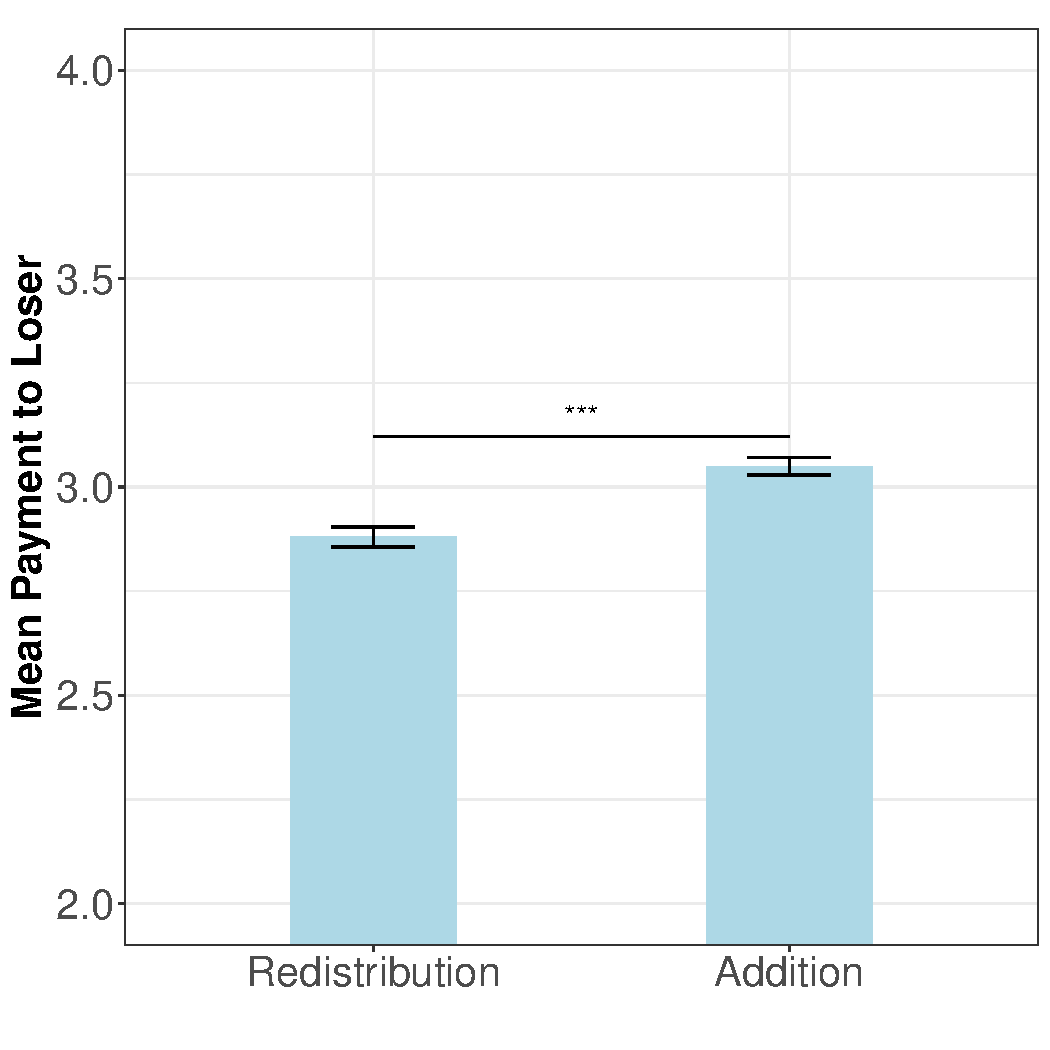
\includegraphics[height=2in]{Figs/payments1.pdf} 
      \caption{Environment initial} \label{environment-initial}
    \end{subfigure}
 \hspace*{6mm}  
 \begin{subfigure}[b]{0.40\textwidth}
   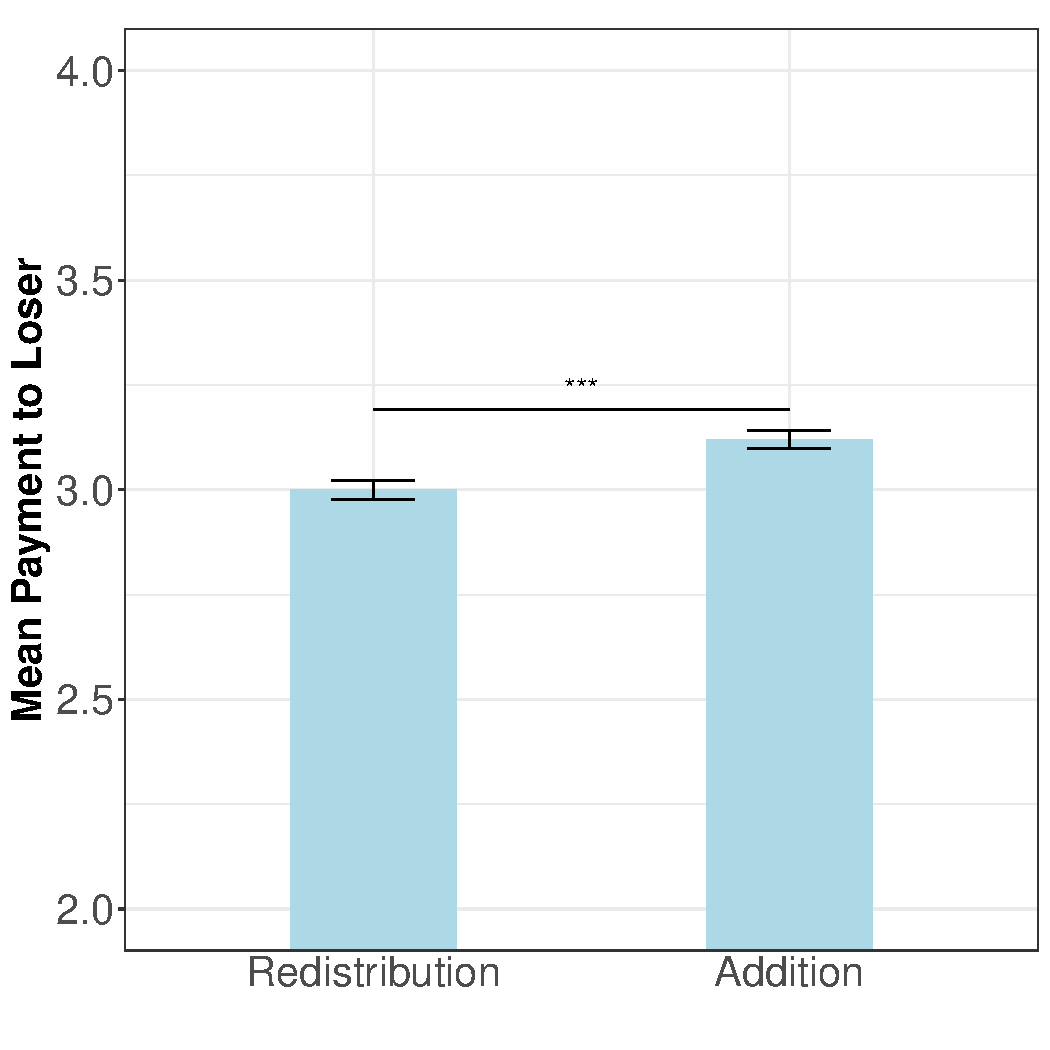
\includegraphics[height=2in]{Figs/payments.pdf} 
      \caption{Environment final} \label{environment-final}
    \end{subfigure}
\hspace*{-10mm}   
 \begin{subfigure}[b]{0.40\textwidth}
      \centering
   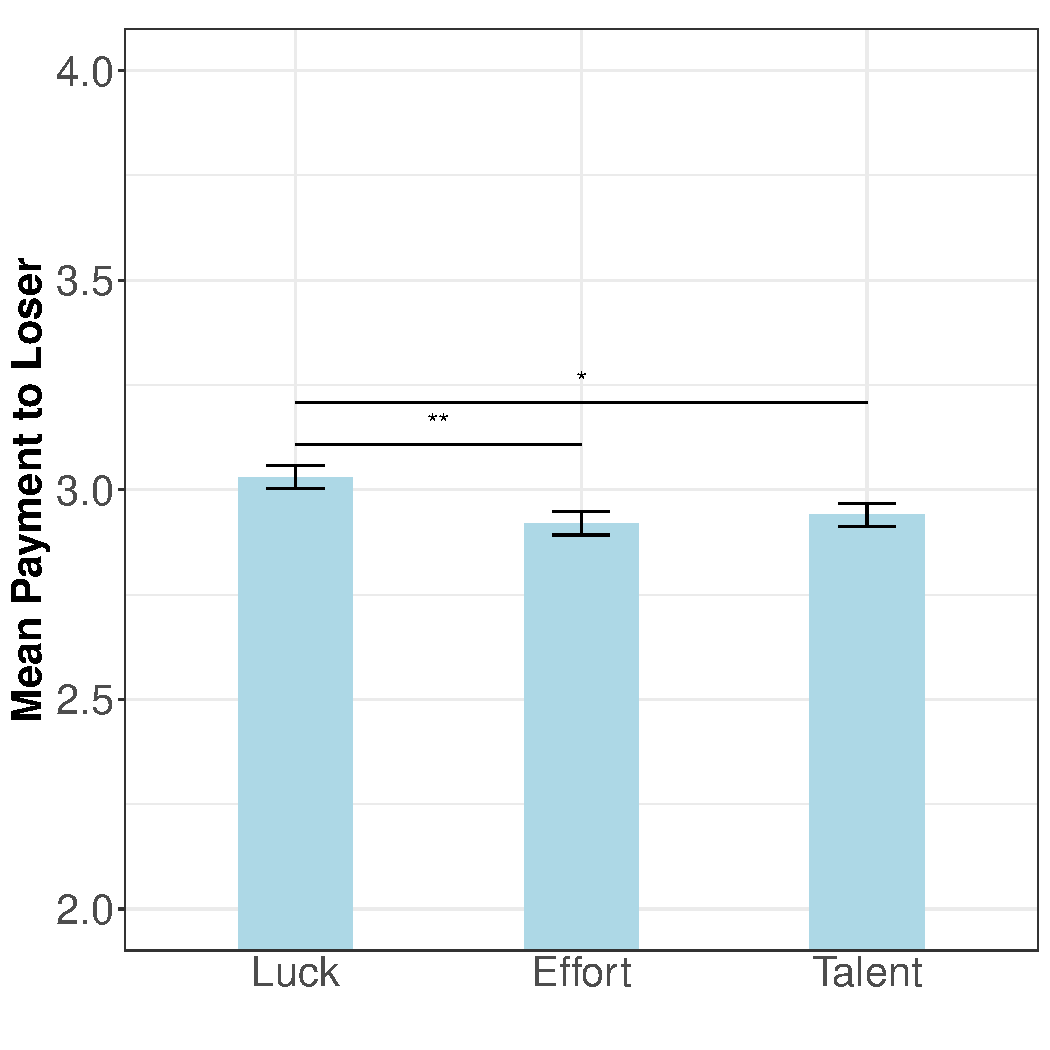
\includegraphics[height=2in]{Figs/paymentsCond1.pdf} 
      \caption{Condition initial} \label{condition-initial}
    \end{subfigure}
 \hspace*{6mm}  
 \begin{subfigure}[b]{0.40\textwidth}
   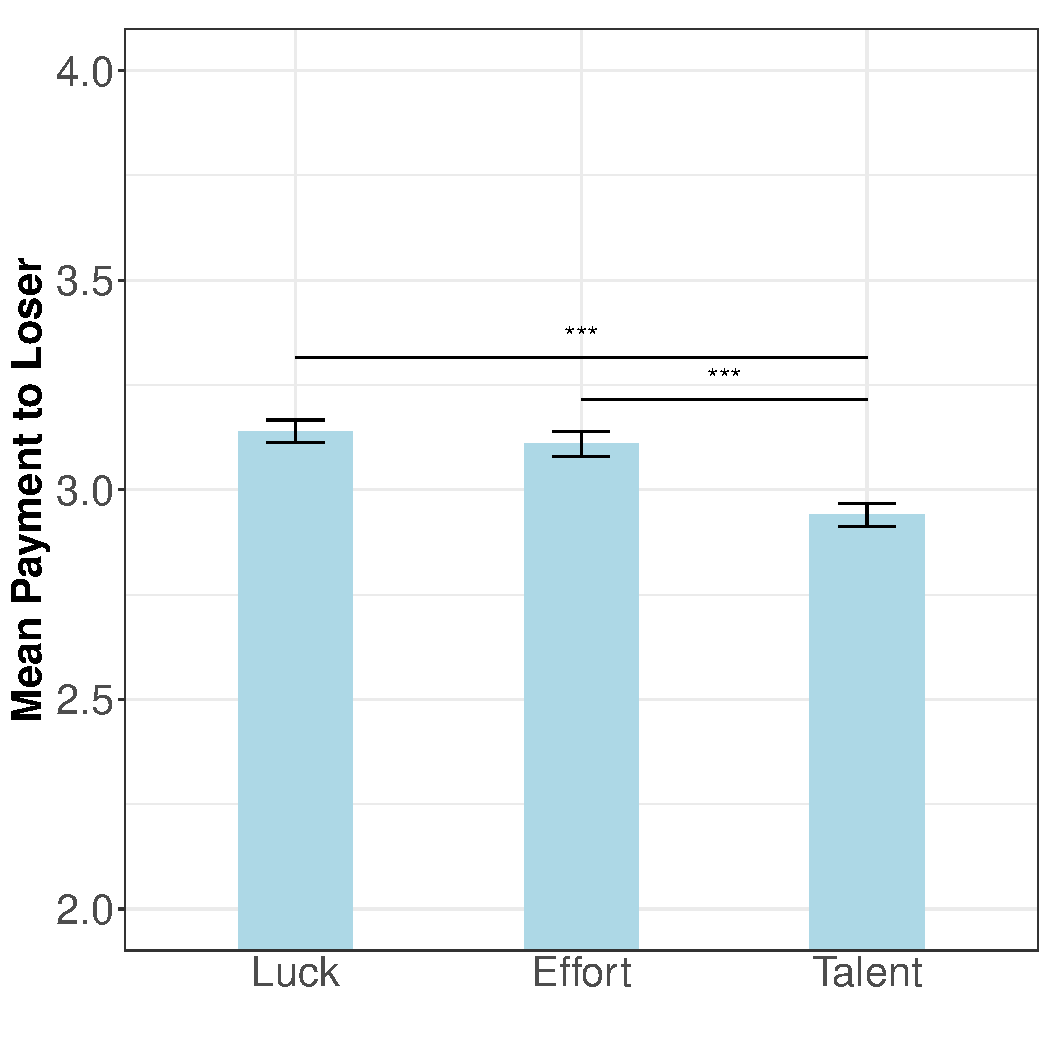
\includegraphics[height=2in]{Figs/paymentsCond.pdf} 
      \caption{Condition final} \label{condition-final}
    \end{subfigure}
\caption{Treatment effects (two-sided Welch t-tests)} \label{superfigure0}
\end{figure} 


Consistent with the literature on inequality acceptance in adults \citep{almaas2020cutthroat}, we observe gender effects, with males exhibiting a stronger preference for meritocracy (transferring less to the loser) compared to females ($p<0.01$). This result contrasts with the findings of \citet{almaas2010fairness}, who studied a related but different game with children and adolescents and reported no gender differences in inequality acceptance. We report a further analysis of gender effects by interacting gender with environment and condition variables in Appendix B2. This analysis shows that interaction effects are generally small.

Additionally, our expectation that children with siblings would allocate more to the losing party—due to their familiarity with adult-induced redistribution—was not supported by the data. Finally, we find no evidence that analytical orientation influences redistribution decisions.\footnote{We interacted these variables with treatments and found no effect. These regressions are omitted for conciseness but can be shared upon request.} We also note a concave age pattern in the final allocation that will be investigated in the next section.


\enlargethispage{2\baselineskip}
\begin{Result}\label{res-treatment} Main treatment estimates. Allocations to the winner are higher:
\begin{itemize}[noitemsep, topsep=0pt, parsep=0pt, partopsep=0pt]
\item[\textbf{a)}] In the redistribution environment.
\item[\textbf{b)}] In the talent condition relative to luck in the pooled final-allocation specification; other source-of-inequality contrasts are less precise.
\item[\textbf{c)}] By male participants.
\end{itemize}
\end{Result}



 
\subsection{Age effects \label{sec-age}}

\subsubsection{Initial allocations}

We now examine age effects in more detail. In \autoref{table-age-initial}, we report OLS regressions where the dependent variable is the \emph{initial allocation to the loser}, and each treatment is separated into its condition and environment components, including interaction terms with age variables.  Figures \ref{initial-redistribution} and \ref{initial-addition} display the quadratic best-fit curves for the initial allocation, plotted as a function of age and winner selection method, separately for the \emph{redistribution} (left) and \emph{addition} (right) environments. 

 
\begin{table}[htpb]
\begin{center}
\begin{footnotesize}
\begin{tabular}{l c c c c c c}
\toprule
 & Redistribution & Redistribution & Addition & Addition & All & All \\
\midrule
\textit{Age}                           & $-0.001$      & $-0.010$      & $0.002^{**}$   & $0.010$        & $0.002^{**}$   & $0.012$        \\
                                       & $(0.001)$     & $(0.008)$     & $(0.001)$      & $(0.007)$      & $(0.001)$      & $(0.007)$      \\
\textit{Age}$^2$                       &               & $0.000$       &                & $-0.000$       &                & $-0.000$       \\
                                       &               & $(0.000)$     &                & $(0.000)$      &                & $(0.000)$      \\
\textit{talent}                        & $0.047$       & $0.047$       & $-0.154^{*}$   & $-0.159^{*}$   & $-0.065$       & $-0.067$       \\
                                       & $(0.099)$     & $(0.096)$     & $(0.088)$      & $(0.088)$      & $(0.069)$      & $(0.067)$      \\
\textit{effort}                        & $-0.063$      & $-0.059$      & $-0.077$       & $-0.081$       & $-0.080$       & $-0.079$       \\
                                       & $(0.097)$     & $(0.098)$     & $(0.090)$      & $(0.088)$      & $(0.067)$      & $(0.066)$      \\
\textit{Male}                          & $-0.110^{**}$ & $-0.106^{**}$ & $-0.169^{***}$ & $-0.170^{***}$ & $-0.147^{***}$ & $-0.144^{***}$ \\
                                       & $(0.045)$     & $(0.044)$     & $(0.050)$      & $(0.050)$      & $(0.034)$      & $(0.033)$      \\
\textit{Siblings}                      & $-0.052$      & $-0.048$      & $-0.020$       & $-0.024$       & $-0.031$       & $-0.032$       \\
                                       & $(0.069)$     & $(0.069)$     & $(0.052)$      & $(0.052)$      & $(0.042)$      & $(0.042)$      \\
\textit{STEM}                          & $0.018$       & $0.012$       & $-0.000$       & $0.005$        & $0.008$        & $0.008$        \\
                                       & $(0.046)$     & $(0.046)$     & $(0.044)$      & $(0.044)$      & $(0.033)$      & $(0.032)$      \\
\textit{redist.}                       &               &               &                &                & $0.249$        & $1.697^{**}$   \\
                                       &               &               &                &                & $(0.194)$      & $(0.690)$      \\
\textit{Age}$\times$\textit{redist.}   &               &               &                &                & $-0.003^{**}$  & $-0.024^{**}$  \\
                                       &               &               &                &                & $(0.001)$      & $(0.010)$      \\
\textit{Age}$^2\times$\textit{redist.} &               &               &                &                &                & $0.000^{**}$   \\
                                       &               &               &                &                &                & $(0.000)$      \\
\midrule
Num. obs.                              & $1078$        & $1078$        & $1163$         & $1163$         & $2241$         & $2241$         \\
Num. groups FE                         & $4$           & $4$           & $4$            & $4$            & $4$            & $4$            \\
Num. clusters SE                       & $62$          & $62$          & $69$           & $69$           & $131$          & $131$          \\
R$^2$                                  & $0.014$       & $0.017$       & $0.043$        & $0.045$        & $0.030$        & $0.035$        \\
Adj. R$^2$                             & $0.006$       & $0.007$       & $0.035$        & $0.037$        & $0.025$        & $0.029$        \\
\bottomrule
\multicolumn{7}{l}{\footnotesize{$^{***}p<0.01$; $^{**}p<0.05$; $^{*}p<0.1$}}
\end{tabular}
\end{footnotesize}
\caption{\textit{Initial} allocation to the loser by treatments and age}
\label{table-age-initial}
\end{center}
\end{table}

  

In the environment-specific regressions (columns 1--4), the estimated developmental patterns differ across environments. In \emph{redistribution}, allocations to the loser are essentially flat with age in both the linear and quadratic specifications. In \emph{addition}, by contrast, allocations to the loser increase with age in the linear specification. In some specifications that allow for curvature, this age pattern is better described as concave---allocations rise with age at younger ages and then level off---though the strength of this curvature depends on whether campus fixed effects are included and on the clustering assumptions (see Appendix B3). We therefore emphasize the difference between the mechanism-specific profiles rather than a precise functional form for the initial allocation.


Additionally, when comparing the developmental patterns across environments (Figures \ref{initial-redistribution} and \ref{initial-addition}), the tendency to allocate resources to the loser in the \emph{addition} environment compared to \emph{redistribution} is stronger among participants in grade 4 and above.

 

 
 
\begin{figure}[htpb]
    \centering

\begin{subfigure}{0.45\textwidth}
    \centering
    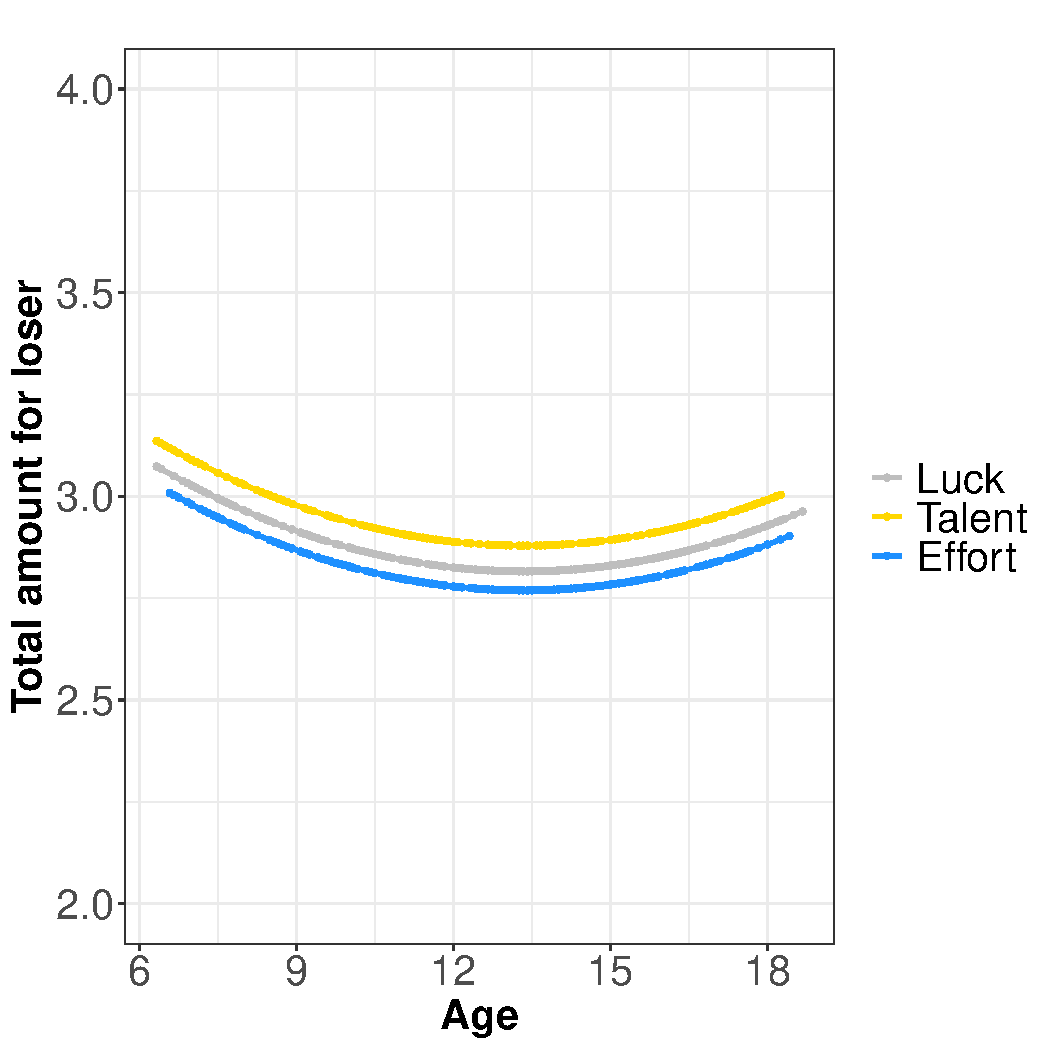
\includegraphics[width=\linewidth]{Figs/redistribution1.pdf}
    \caption{Redistribution}
    \label{initial-redistribution}
\end{subfigure}
\hfill
\begin{subfigure}{0.45\textwidth}
    \centering
    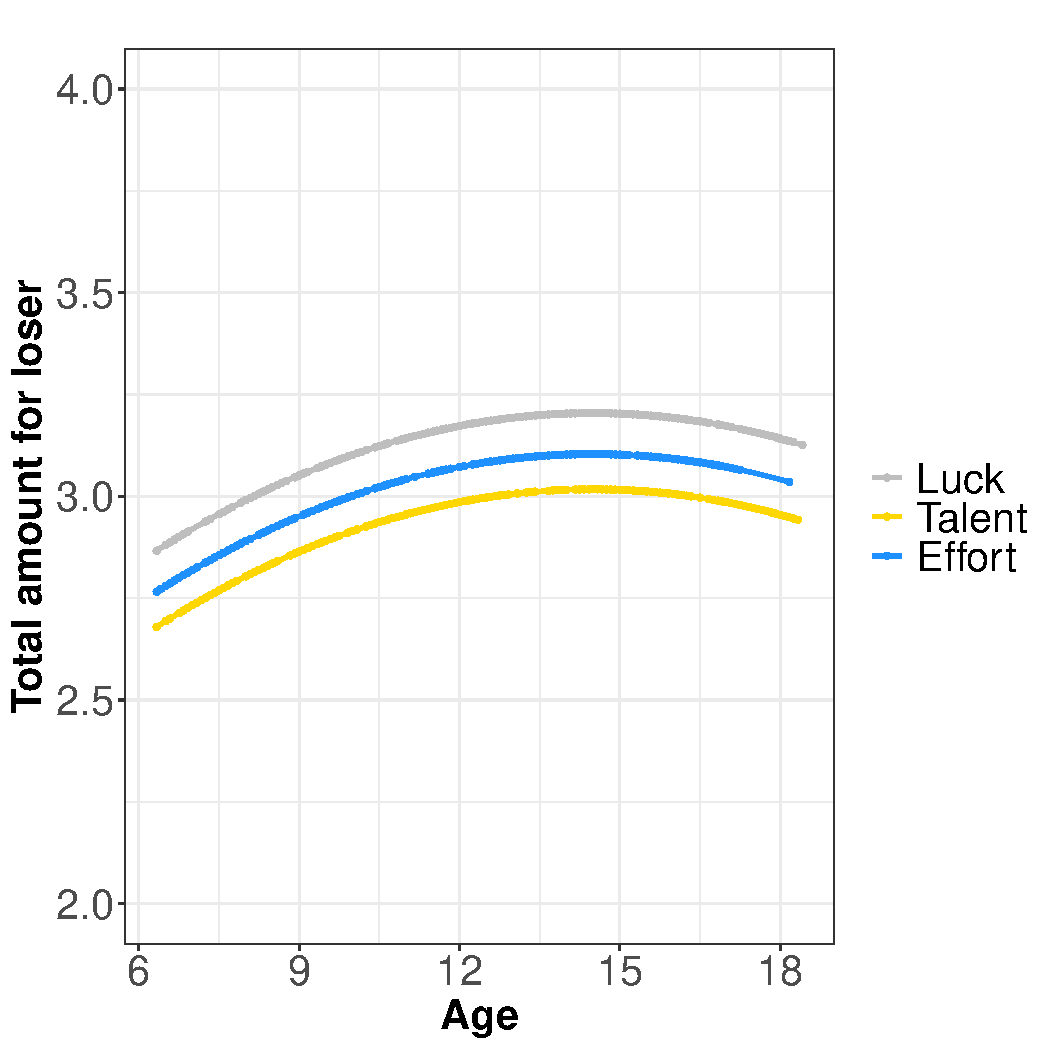
\includegraphics[width=\linewidth]{Figs/addition1.pdf}
    \caption{Addition}
    \label{initial-addition}
\end{subfigure}

\caption{$Initial$ allocation to the loser across ages}
\label{superfigure1}
\end{figure}
 
 

To test whether developmental profiles differ across environments, columns 5--6 in \autoref{table-age-initial} pool the data and interact $Age$ (and, in column 6, $Age^2$) with the \emph{redistribution} indicator. In these pooled models, the coefficient on \emph{Age} (and $Age^2$) captures the developmental profile in the \emph{addition} environment (the reference environment), while the interaction terms indicate how the \emph{redistribution} profile departs from it. The negative and statistically significant $Age$$\times$$redistribution$ interaction indicates that the age-related increase estimated under \emph{addition} is weaker under \emph{redistribution}. In the quadratic specification, the interaction estimates are also consistent with different curvature across environments. Because $Age$ is measured in months, the main effect of \emph{redistribution} in the pooled specifications reflects differences evaluated at the smallest age and is not directly interpretable; this is why we focus on the implied age profiles and interaction terms rather than on the redistribution intercept.\footnote{Appendix B3 shows that the qualitative distinction between a comparatively flat profile in \emph{redistribution} and an increasing, sometimes concave profile in \emph{addition} appears across several alternative specifications. The exact curvature and its precision are specification-dependent. Appendix B4 reports estimates using age-group indicators.}

\begin{Result} \label{res-initial} For the initial choices: 
\noindent \begin{itemize}[noitemsep, topsep=0pt, parsep=0pt, partopsep=0pt]
\item[\textbf{a)}] The estimated allocation to losers is comparatively flat with age under redistribution and increasing under addition. Evidence on concavity in the initial allocation depends on the econometric specification.
\item[\textbf{b)}] The tendency to allocate more resources to losers under addition than under redistribution is stronger among participants in grade 4 and above.
\item[\textbf{c)}] Male participants allocate fewer resources to losers.

\end{itemize}
\end{Result}

\subsubsection{Final allocations}


\autoref{table-age-final} and \autoref{superfigure} report the analogue of \autoref{table-age-initial} and \autoref{superfigure1} for the \emph{final} decision. As before, Appendix B3 replicates the analysis under alternative specifications, and Appendix B4 replaces $Age$ in months with \emph{Age-group} indicators. Remember that between the initial and final choices, observers experienced the tournament, allowing them to assess the task's difficulty and their expected performance. However, they were not informed of their actual outcome, and the design did not allow for any form of reciprocity. And yet, one might expect that experiencing the task could influence behavior, for example, by increasing empathy toward the loser if the participant perceived it as difficult or believed they underperformed. In practice, approximately two-thirds of participants did not revise their initial allocation.\footnote{\label{foot-equal}In \emph{addition}, 79\% (luck), 69\% (effort) and 67\% (talent) of participants did not revise their initial allocation. In \emph{redistribution}, 66\% (luck), 61\% (effort) and 65\% (talent) did not revise it.}




\begin{table}[htpb]
\begin{center}
\begin{footnotesize}
\begin{tabular}{l c c c c c c}
\toprule
 & Redistribution & Redistribution & Addition & Addition & All & All \\
\midrule
\textit{Age}                           & $0.001$        & $0.002$        & $0.002^{**}$   & $0.019^{**}$   & $0.002^{**}$   & $0.021^{***}$  \\
                                       & $(0.001)$      & $(0.007)$      & $(0.001)$      & $(0.007)$      & $(0.001)$      & $(0.007)$      \\
\textit{Age}$^2$                       &                & $-0.000$       &                & $-0.000^{**}$  &                & $-0.000^{***}$ \\
                                       &                & $(0.000)$      &                & $(0.000)$      &                & $(0.000)$      \\
\textit{talent}                        & $-0.215^{***}$ & $-0.215^{***}$ & $-0.128$       & $-0.139^{*}$   & $-0.177^{***}$ & $-0.183^{***}$ \\
                                       & $(0.075)$      & $(0.076)$      & $(0.083)$      & $(0.078)$      & $(0.058)$      & $(0.056)$      \\
\textit{effort}                        & $-0.085$       & $-0.085$       & $0.046$        & $0.037$        & $-0.026$       & $-0.030$       \\
                                       & $(0.091)$      & $(0.091)$      & $(0.090)$      & $(0.086)$      & $(0.067)$      & $(0.065)$      \\
\textit{Male}                          & $-0.105^{*}$   & $-0.106^{*}$   & $-0.204^{***}$ & $-0.206^{***}$ & $-0.158^{***}$ & $-0.159^{***}$ \\
                                       & $(0.056)$      & $(0.056)$      & $(0.044)$      & $(0.043)$      & $(0.035)$      & $(0.035)$      \\
\textit{Siblings}                      & $-0.020$       & $-0.020$       & $-0.066$       & $-0.073$       & $-0.040$       & $-0.045$       \\
                                       & $(0.058)$      & $(0.058)$      & $(0.065)$      & $(0.062)$      & $(0.044)$      & $(0.043)$      \\
\textit{STEM}                          & $0.021$        & $0.023$        & $-0.002$       & $0.009$        & $0.008$        & $0.015$        \\
                                       & $(0.051)$      & $(0.051)$      & $(0.044)$      & $(0.043)$      & $(0.034)$      & $(0.033)$      \\
\textit{redist.}                       &                &                &                &                & $0.118$        & $1.536^{**}$   \\
                                       &                &                &                &                & $(0.204)$      & $(0.741)$      \\
\textit{Age}$\times$\textit{redist.}   &                &                &                &                & $-0.001$       & $-0.022^{**}$  \\
                                       &                &                &                &                & $(0.001)$      & $(0.010)$      \\
\textit{Age}$^2\times$\textit{redist.} &                &                &                &                &                & $0.000^{**}$   \\
                                       &                &                &                &                &                & $(0.000)$      \\
\midrule
Num. obs.                              & $1078$         & $1078$         & $1151$         & $1151$         & $2229$         & $2229$         \\
Num. groups FE                         & $4$            & $4$            & $4$            & $4$            & $4$            & $4$            \\
Num. clusters SE                       & $62$           & $62$           & $68$           & $68$           & $130$          & $130$          \\
R$^2$                                  & $0.028$        & $0.028$        & $0.049$        & $0.060$        & $0.033$        & $0.041$        \\
Adj. R$^2$                             & $0.019$        & $0.019$        & $0.041$        & $0.052$        & $0.028$        & $0.036$        \\
\bottomrule
\multicolumn{7}{l}{\footnotesize{$^{***}p<0.01$; $^{**}p<0.05$; $^{*}p<0.1$}}
\end{tabular}
\end{footnotesize}
\caption{\textit{Final} allocation to the loser by treatments and age}
\label{table-age-final}
\end{center}
\end{table}




\begin{figure}[htpb]
    \centering

\begin{subfigure}{0.45\textwidth}
    \centering
    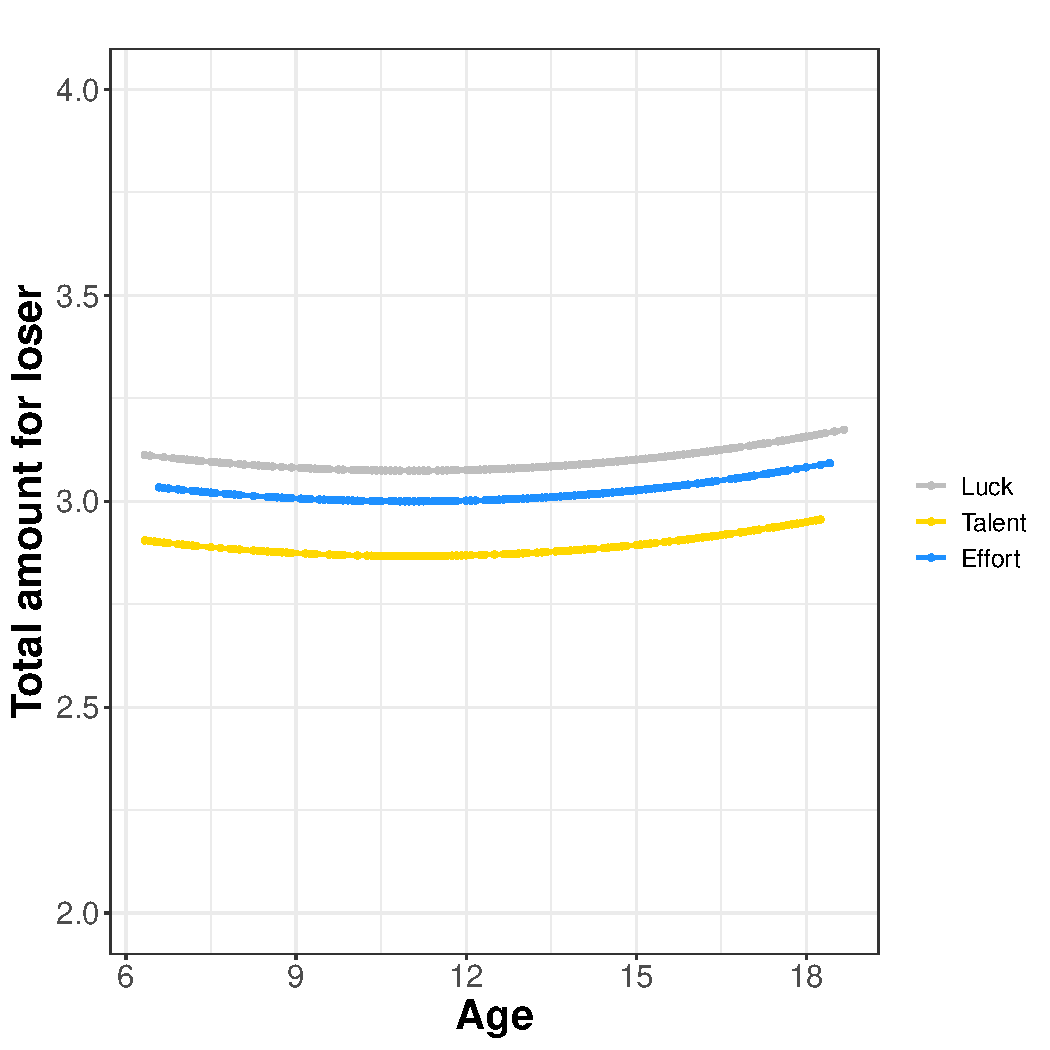
\includegraphics[width=\linewidth]{Figs/redistribution.pdf}
    \caption{Redistribution}
    \label{superfigure-redist}
\end{subfigure}
\hfill
\begin{subfigure}{0.45\textwidth}
    \centering
    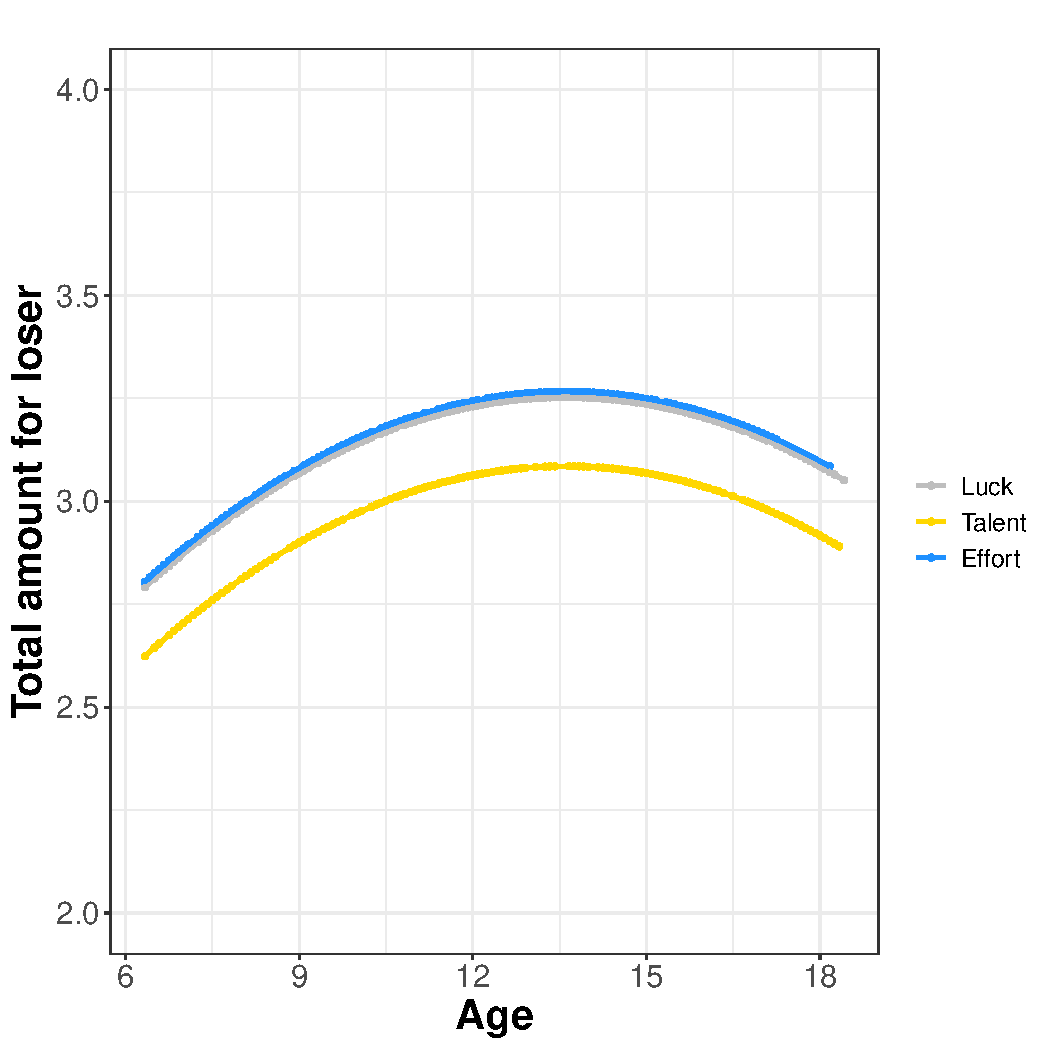
\includegraphics[width=\linewidth]{Figs/addition.pdf}
    \caption{Addition}
    \label{superfigure-addit}
   \end{subfigure}

\caption{$Final$ allocation to the loser across ages}
\label{superfigure}
\end{figure}






In \emph{redistribution}, final allocations display the same developmental pattern as initial choices: neither $Age$ nor $Age^2$ significantly predict allocations to the loser in the environment-specific regressions. In contrast with the initial decision, however, the \emph{talent} condition is now associated with a sizable reduction in the loser’s final allocation relative to \emph{luck}, whereas \emph{effort}  remains statistically indistinguishable from \emph{luck}. These conclusions are confirmed by the pooled specifications with age-by-environment interactions.

In \emph{addition}, the final allocation increases with age in the linear specification and is concave in the quadratic specification. Regarding winner-selection conditions, the point estimates for \emph{talent} and \emph{effort} (relative to \emph{luck}) are smaller and less precisely estimated within addition than within redistribution, while the pooled regressions indicate that, on average, \emph{talent} is associated with lower allocations to the loser.

The last two columns pool both environments and test whether developmental profiles differ across \emph{addition} and \emph{redistribution} by interacting the age variables with the redistribution indicator. In these regressions, the coefficients on $Age$ and $Age^2$ describe the age profile in the \emph{addition} environment (the reference), while the interaction terms capture how the \emph{redistribution} profile departs from it. In the quadratic specification, the negative and statistically significant $Age\times$\emph{redistribution} interaction, together with the offsetting curvature term, indicates that the age-related increase and concavity estimated under \emph{addition} are attenuated under \emph{redistribution}, consistent with a near-flat redistribution profile. Again, because $Age$ is measured in months, the standalone redistribution coefficient corresponds to the difference evaluated at the smallest age and is not directly interpretable; we focus on the implied profiles and interaction terms. Appendix B3 reports qualitatively similar estimates across specifications with session/classroom-level clustering. With clustering at the campus level, standard errors become more conservative given the small number of campuses, while the point estimates remain similar.

As before, male participants display more meritocratic preferences. These patterns persist if we run separate regressions for each winner selection method (see Appendix B5 and B6 for details).


\begin{Result} \label{res-final}
For choices made after experiencing the competition task:
\noindent \begin{itemize}[noitemsep, topsep=0pt, parsep=0pt, partopsep=0pt]
\item[\textbf{a)}] Estimated final transfers to losers are comparatively flat with age under redistribution, whereas the quadratic specification under addition peaks around age fourteen.
\item[\textbf{b)}] Point estimates suggest a stronger winner-favoring pattern in the talent condition among participants in grade 4 and above, but these finer age-by-condition comparisons are less precise.
\item[\textbf{c)}] Male participants remain more likely to favor the winner than female participants.
\end{itemize}
\end{Result}
 

\subsection{What makes subjects revise their initial decision? \label{sec-revise}}

Final choices are made after participants have experienced the competition task and have been invited to reconsider their initial allocation. We next document correlates of the shifts in choices. Because the design has no control group that repeats the allocation without task participation, these estimates do not isolate a causal effect of competitive experience from reflection, reconsideration, or repeated measurement.

During the experiment, we included two sets of non-incentivized questions regarding the  participants’ perceptions about the level of difficulty of the competition task and their performance relative to others. These questions were not included in the \emph{luck} condition, as the winner was randomly determined. We expected to observe self-serving biases among participants: those who perceived their performance as higher than others and found the task easy would likely lean towards more meritocratic allocations (and vice versa).\footnote{One must acknowledge the exogenous limits to this tendency, as individuals who initially choose (4,4) and (6,2) cannot shift towards more and less redistribution, respectively.}

For our analysis, we consider each allocation method and each initial choice separately: meritocratic (6,2), equitable (5,3) and compensatory (4,4). For initial meritocratic (Merit.) and compensatory (Comp.) choices, we perform Poisson regressions, where we interpret the absolute value of the change in the allocation to the winner between the initial and final choice as counts $(0,1,2)$.
For initial equitable choices (Equit.), we perform a multinomial regression of the likelihood to decrease $(-1)$ or increase $(+1)$ the final allocation of the winner. Thus, a positive coefficient in Merit.\ and Equit.$(-1)$ implies an increase in the allocation to the loser whereas a positive coefficient in Comp.\ and Equit.$(+1)$ implies an increase in the allocation to the winner. We include all the previous  dependent variables 
and excluded data from \emph{luck}. 
We pool data from \emph{effort} and \emph{talent} with a \emph{talent} dummy. 

Regarding our variables of interest, we use ``equal / I don't know" as the reference category for participants’ self-reported perceived performance and introduce dummies for $better$ and $worse$. Similarly, for self-reported perceived difficulty, we set ``same / I don't know" as the reference and include dummies for $hard$ and $easy$. \autoref{fig-change-all} presents the corresponding regression results.

\input{Figs/table5.tex}

Perceived own performance is associated with revisions in several specifications, although not all individual transitions are statistically distinguishable from zero. Participants who believed that they performed better were generally less likely to move away from a meritocratic initial allocation and more likely to move from equitable toward meritocratic allocations. For the equitable-to-compensatory contrast in the addition environment, however, the estimated association with perceived better performance is not statistically significant. Associations with perceived worse performance are often in the opposite direction, particularly in addition. Perceived task difficulty is less consistently related to revisions. 
For instance, the estimated hard-task coefficient for the equitable-to-compensatory contrast in the addition environment is not statistically significant. The multinomial model for initial equitable choices in addition also exhibits an empty outcome-by-covariate cell: no participant reporting worse performance moved from equitable to meritocratic allocation. The corresponding large negative coefficient and near-zero reported standard error should not be interpreted as conventional statistical evidence. 
This pattern is consistent with an egocentric interpretation and with some existing findings in the literature. For example, \citet{neuber2021egocentric} found that individuals engaged in distributing rewards to others often adhere to norms that favor their own interests, even in situations where their choices exclusively impact others. Since perceived performance and difficulty are self-reported, however, the estimates should be read as associations rather than as causal effects.

\begin{Result} \label{res-perception}
Revisions are consistent with a self-serving pattern: individuals who perceived their performance as above others' and considered the task easy tended to revise allocations in favor of the winner.
\end{Result}
 
\subsection{Non-cognitive abilities and decision-making \label{sec-noncog}} \label{sec-noncog-and-choice}

Recent research has found that cognitive abilities shape our time and risk preferences \citep{dohmen2010risk}, although the exact mechanism is still not fully understood \citep{amador2021cognitive}. In this study we take a different route and hypothesize a link between non-cognitive abilities --empathy and personality-- and social preferences. Empathy and personality are measured with the DeRMET and P-Big 5 tasks described in section \ref{sec-design}. Performance by age is summarized in \autoref{fig-noncog} and discussed in the Appendices, which also provide validation and comparative analyses of $DeRMET$ (Appendix B7) and $P$-$Big$ $5$ (Appendix B8).


 \begin{figure}[htpb]
\vspace*{-10mm}
\hspace*{-16mm}
\centering
\makebox[\textwidth]
{\makebox[1.15\textwidth]{
    \begin{minipage}{.48\textwidth}
        \centering
        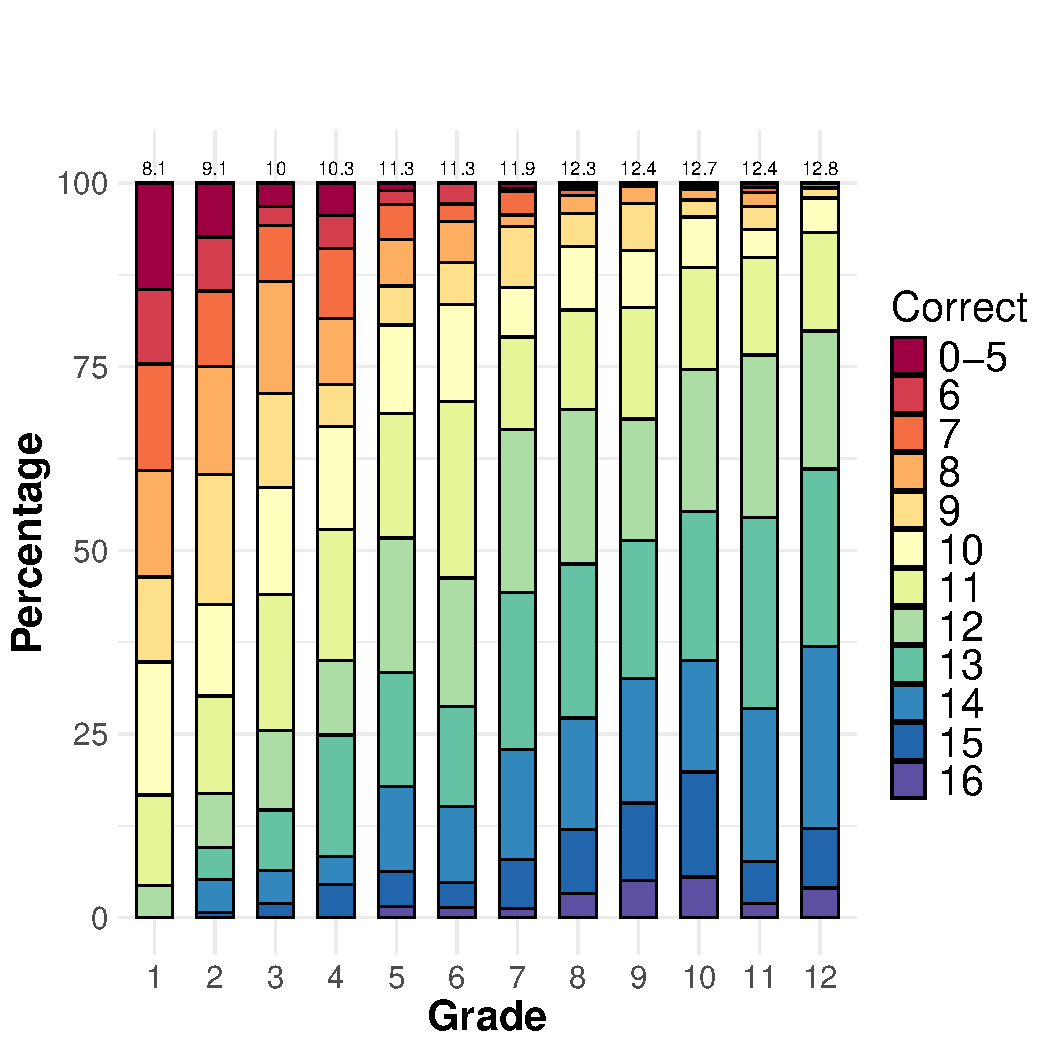
\includegraphics[width=0.85\textwidth]{Figs/fig-tom-dist.pdf}
     \end{minipage}\hfill
    \begin{minipage}{.64\textwidth}
        \centering
        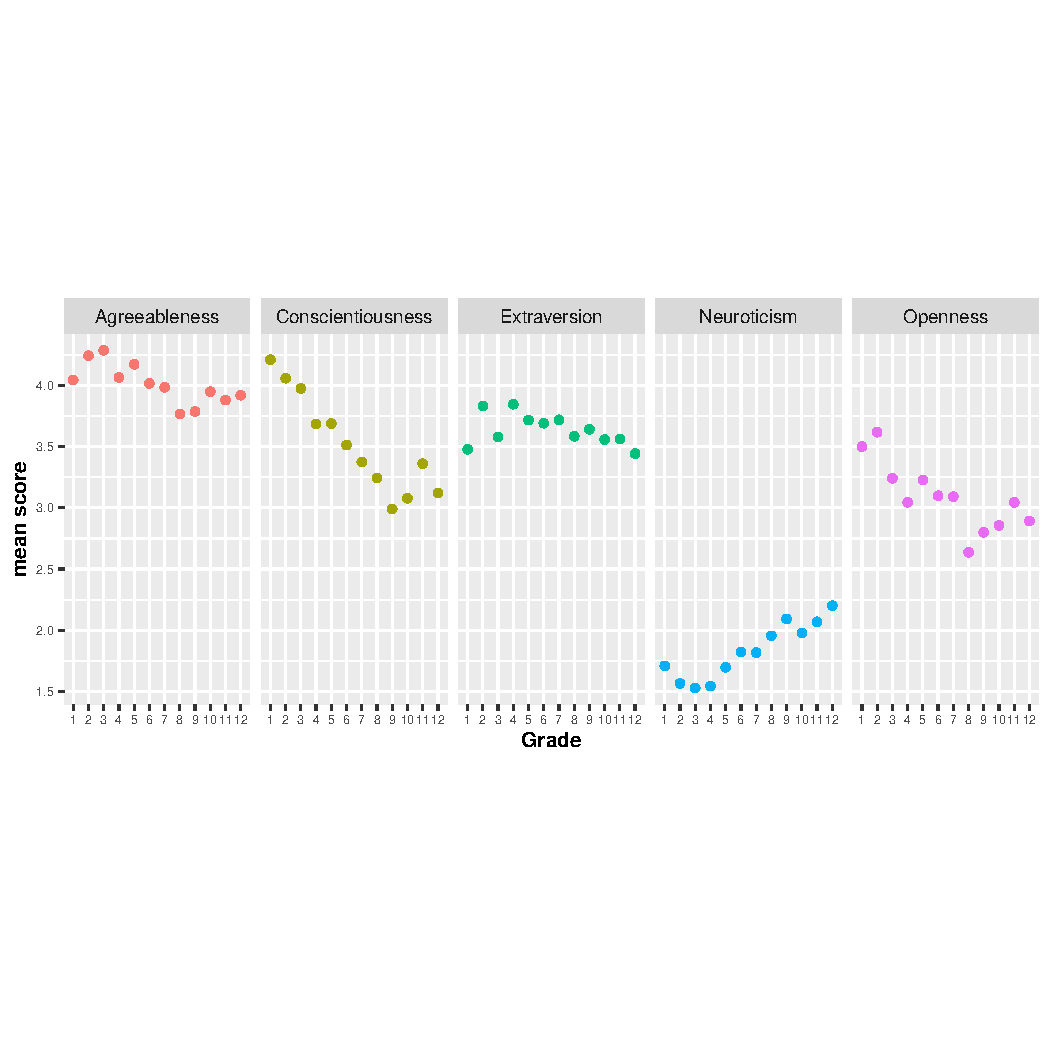
\includegraphics[width=1.1\textwidth]{Figs/fig-big5-score.pdf}
        \end{minipage} 
}}
\vspace{-7mm}
\caption{Left: Distribution of correct answers in DeRMET by grade with grade average on top. Right: Average score in the P-Big 5 by trait and grade} \label{fig-noncog}
\end{figure}

In line with the existing literature, we find sustained and statistically significant changes in empathy  and personality scores with age. At the same time, both tasks are very revealing: the empathy test is neither trivial nor exceptionally difficult for any age, and the results of our pictorial personality test align well with the answers to the standard verbal questionnaires (see Appendices B7 and B8).


To examine the interplay between the ability to interpret emotions, individual personality traits, and meritocratic decision-making, we estimate multinomial regressions using the ``equitable" allocation (5,3) as the reference category. The dependent variables include ``Merit." and ``Comp.", that is, choosing instead (6,2) and (4,4) respectively.

To enhance statistical power, we pool data from all variants. We include dummies for treatment (\emph{redistribution}, with \emph{addition} as the reference) and winner selection method (\emph{luck} and \emph{talent}, with  \emph{effort} as the reference), and the usual control variables ($Age$, $Age^2$, $Male$, $Siblings$, $STEM$). For each individual, we assess the number of correct answers in the DeRMET and their responses to the P-Big 5. To control for age-related trends and extract individual specific traits, we first regressed each score on age and use the residuals as our dependent variables (\emph{resid}) in our regression. We carry out the regressions for both the initial and final choices.\footnote{We also ran the analysis using standardized scores to reflect differences in scores relative to peers in the same grade. The results are very similar in both magnitude and significance of effects.} The results are presented in \autoref{table-ToMandBig5}.



Participants with higher DeRMET scores show a significant decrease in their likelihood of initially choosing the meritocratic allocation over the equitable one. This suggests that a stronger ability to interpret others’ emotions is associated with greater empathy toward disadvantaged individuals, even when the inequality stems from the participants' own actions. However, this effect fades when it comes to the final decision. As participants engage with the task and gain personal experience, their choices become increasingly shaped by their own performance (as discussed in Section \ref{sec-revise}), which appears to offset the initial emotional considerations.

Personality also plays a significant role in shaping decisions. \emph{Conscientiousness} is linked to a greater likelihood of making meritocratic choices in the final stage, while \emph{agreeableness} is associated with a preference for less meritocratic choices, both in the initial and final decisions. \emph{Openness} is connected to an inclination for compensatory choices, although this association is mainly observed in the initial stage. These findings align with prior research linking conscientiousness to a preference for right-wing political parties and openness to a preference for left-wing political parties \citep{vecchione2011personality, furnham2018personality, ekstrom2019personality}.


Allowing traits to jointly moderate the effects of the environment and the winner-selection condition, we find that most high-order interactions are imprecisely estimated. Statistically significant three-way interactions are few and do not point to a pervasive pattern, suggesting limited systematic heterogeneity beyond the main treatment contrasts (see Appendix B9 for details). 

We also report in Appendix B10 regression analysis of change between initial and final choices. Performance in $DeRMET$ is only weakly related to revisions once task perceptions are controlled for, and the two marginally significant associations point in opposite directions. Personality traits are more systematically related to revision patterns, even conditional on perceived performance and difficulty. Higher $Extraversion$ is associated with persistence in winner-favoring allocations in the \emph{redistribution} environment. In the \emph{addition} environment, higher $agreeableness$ is associated with persistence in compensatory allocations, higher $Openness$ with fewer transitions from equitable allocations toward the loser (Equit.$(-1)$), and lower $Conscientiousness$ with revisions toward the loser.

Finally, we notice that the tendency for males to display a stronger preference for meritocratic allocations remains significant even after controlling for $DeRMET$ performance and personality attributes. 

\Needspace{8\baselineskip}
\begin{Result} \label{res-noncog} 

\noindent \begin{itemize}[noitemsep, topsep=0pt, parsep=0pt, partopsep=0pt]



\item[\textbf{a)}] Participants with higher emotional intelligence are less likely to initially exhibit meritocratic preferences. 
\item[\textbf{b)}] As for personality, conscientiousness is linked to a greater likelihood of making meritocratic final choices while agreeableness has the opposite effect.
\item[\textbf{c)}]  Male participants are more likely to be meritocratic in both initial and final decisions.
\end{itemize}

\end{Result}

\input{Figs/Table6.tex}


\subsection{Crosswalk from empirical contrasts to model primitives}

The conceptual framework is not introduced to ``explain away'' the data, but to organize possible interpretations of the experimental contrasts. The design varies two dimensions: token allocation environment and winner selection method. In the model, the first dimension is represented by a potential aversion to taking resources from parties ($d$), the second by shifts in the merit weight ($m_z$), and within-subject revisions by updating on deservingness ($m_z'$). These interpretations require assumptions that the experiment does not separately test. Table \ref{tab:crosswalk} maps each empirical pattern to its corresponding model representation.

\begin{table}[htpb]
\footnotesize
\caption{Crosswalk from empirical contrasts to model primitives}
\label{tab:crosswalk}
\hspace*{-6mm}\begin{tabularx}{1.10\linewidth}{p{0.42\linewidth} p{0.15\linewidth} X}
\toprule
\textbf{Empirical contrast / main finding} &
\textbf{Model \quad primitive} &
\textbf{Interpretation within the model} \\
\midrule

Redistribution v.\ addition: loser receives less under redistribution (initial and final)  &
$d$ &
Consistent with procedural disutility $d>0$ (taking compresses equalization).\medskip \\ 

Luck v.\ effort v.\ talent: allocations are most meritocratic under talent; effort $\approx$ luck &
$m_z$ &
Point estimates are consistent with a larger merit weight under talent, especially relative to luck; the effort contrasts are imprecise.\medskip\\

Age gradients differ by mechanism: concavity in addition; flat profile in redistribution &
$m_z(\text{age}),\, d(\text{age})$ &
Mechanism-specific age profiles can be represented by age variation in $m_z$ and $d$; the data do not separately identify these channels.\medskip\\

Within-subject revision: direction correlates with perceived performance &
$\alpha$ &
Revisions correlated with perceptions are consistent with updating, but also with reconsideration or repeated measurement.\medskip\\

Gender (Male): allocations are more meritocratic 
& $m_z(\text{gender})$ 
& Baseline heterogeneity in the merit weight: $m_z(\text{male}) > m_z(\text{female})$.\medskip\\



Non-cognitive traits: heterogeneity in allocations and/or moderation of treatment effects &
$m_z$ (and possibly $d,\alpha$) &
Shifts in baseline $m_z$ and $\alpha$; trait$\times$ condition interactions: shifts in $m_z$ across conditions. No effect on $d$.\medskip\\

\bottomrule
\end{tabularx}
\end{table}

The results in sections \ref{sec-treat}, \ref{sec-age} and \ref{sec-revise} offer the following interpretations. First, the allocation procedure matters: lower transfers to losers under redistribution are consistent with a positive procedural-disutility term in our model ($d>0$). Almost one-third of our subjects revise their initial allocation. The correlation between these revisions and perceived performance is consistent with updating, but the design cannot distinguish updating from reconsideration or repeated measurement.


Point estimates also suggest a higher merit weight under talent than under luck, especially for the final allocation; the effort estimates are less precise.
Finally, we observe two estimated developmental patterns depending on the mechanism. Within the model, this may reflect a tension between fairness preferences and procedural disutility. Under \emph{addition}, the procedural-disutility term is moot since $x_W>x_W^o$ and $x_L>x_L^o$ by design; under \emph{redistribution}, it may offset developmental changes in fairness preferences. This is one interpretation of the mechanism-specific profiles rather than a separately identified causal channel.

Regarding gender, the fact that males are systematically more meritocratic is most naturally read as a higher baseline merit weight for males, i.e. $m_z(\textrm{male})>m_z(\textrm{female})$. This gap holds both in the initial and final choices, and remains when controlling for DeRMET and Big-5 traits. However, we do not detect differential sensitivity to the environment (the coefficient for the interaction \emph{Male}$\times$\emph{Redistribution} is small and insignificant). Still, the significant \emph{Effort}$\times$\emph{Male} effect in the final allocation indicates that the effort condition shifts the implied merit weight $m$ differently for males than for females. By contrast, there is no evidence that gender operates through $d$ in our data.
 

Last, variation in non-cognitive traits create systematic heterogeneity in allocations and/or moderate treatment effects. 
Empirically, higher DeRMET (emotional recognition/empathy) is associated with a lower propensity to choose the meritocratic split in the \emph{initial} allocation, but this association largely vanishes in the \emph{final} decision, consistent with experience-based updating between choices. In contrast, personality traits exhibit more persistent patterns: conscientiousness is linked to more meritocratic choices (higher $m$), agreeableness to less meritocratic choices (lower $m$), and openness to a greater tendency towards egalitarian allocations, with effects concentrated mainly at the initial stage. 
The weak \emph{trait}$\times$\emph{environment} interactions suggest that there is little evidence that $d$ varies systematically with individual characteristics once we allow for rich interactions. By contrast, the significance of several \emph{trait}$\times$\emph{conditions} terms point to 
trait-dependent shifts in the merit weight across conditions. 

We also find evidence that several traits predict systematic revision biases. Specifically, Extraversion, Agreeableness, Conscientiousness, and Openness are the traits most consistently associated with revision patterns across specifications. The association between DeRMET and revisions is weak and not uniform in direction.



\section{Conclusion} \label{sec-conclusion}

In this study, impartial observers aged 6 to 18 in Spain decide the allocation of rewards between a winner and a loser. We examined three (between-subject) conditions for determining the winner --\emph{effort}, \emph{talent}, and \emph{luck}--, two (between subjects)  methods for allocating rewards --\emph{redistribution\/}  and \emph{addition}--, and two (within subject) timings for choice --before and after experiencing the task. 

Participants in all age groups allocated less to the loser when equalization required actively reducing the winner's tokens. Under \emph{addition}, the estimated age profile of final allocations rose through middle school and declined afterwards; under \emph{redistribution}, it was comparatively flat. In pooled final-allocation specifications, observers allocated less to the loser when the winner was determined through \emph{talent} rather than \emph{luck}; the estimates for \emph{effort} relative to \emph{luck} were small or imprecise. Revisions were associated with participants' perceptions of their own performance and task difficulty, but the design does not isolate task experience from reconsideration. Individual characteristics and non-cognitive traits were also related to decisions. In particular, male participants exhibited more meritocratic allocations in both their initial and final choices.

Overall, the study jointly examines how responses to the origin of inequality and to redistribution mechanisms vary between childhood and late adolescence. The estimates indicate an early sensitivity to both outcomes and procedures, while also showing that the precision of finer treatment-by-age comparisons is limited. A few additional remarks are in order.

 

The lower allocation to the loser under redistribution than under addition is consistent with an aversion to intervention, reminiscent of status quo bias \citep{kahneman1991anomalies}, and complements the effect documented by \citet{list2007interpretation}. The designs are distinct: List expands the action set of self-interested adult dictators to include taking, whereas our impartial observers choose between the same three final allocations under both mechanisms. Our evidence therefore suggests that procedural sensitivity extends to third-party judgments and is already present among children and adolescents. One possible interpretation is observer-side loss aversion: taking from a winner may be coded as a loss-creating act. The experiment does not uniquely identify this mechanism, but it raises the possibility that institutionally equivalent allocations may be viewed differently depending on how they are implemented.

Our sample covers ages 6 to 18 and therefore speaks directly to childhood and adolescence, not to later stages of the life cycle. Evidence from self-interested dictator games indicates that age patterns can continue to change in adulthood and older age, although the direction depends on the paradigm. For example, \citet{cobo2019development} report non-linear changes in egalitarian and altruistic types between ages 9 and 67, while the meta-analysis by \citet{engel2011dictator} finds greater giving in older subject pools. These findings are useful benchmarks but are not directly comparable to impartial-observer choices. Whether the mechanism-specific profiles documented here persist, converge, or reverse in adulthood and old age remains an open question.

Between 20\% and 40\% of observers reassessed their choices after engaging in the competition task and being invited to reconsider their initial allocation. These revisions are systematically associated with participants' own perceptions of performance. This pattern is consistent with experiential learning \citep{kolb2014experiential}, but also with reflection or repeated measurement. Task participation may provide information about difficulty and the requirements for success, while also introducing subjective anchors. In our setting, perceived own performance is strongly associated with revisions. Similar patterns may arise in other decision-making paradigms where participants take on roles different from their own.


The talent--luck point estimates, clearest in the pooled final-allocation specifications, suggest a tendency to reward winners perceived as more deserving. The evidence is less precise for effort, and we therefore do not interpret the estimates as establishing a general ranking of talent, effort, and luck. The result nevertheless suggests that sensitivity to the perceived source of inequality may emerge early in life.


The importance of the source of inequality aligns with previous findings  \citep{cappelen2010responsibility}, and has been sometimes linked to political affiliations and individual characteristics \citep{alesina2011preferences, luttmer2011culture, almaas2020cutthroat}. In our case, we are able to link individual heterogeneity with non-cognitive skills. Participants with a higher capacity for empathy exhibit lower levels of merit-based choices.
Similarly, individuals who score higher on agreeableness and openness and lower on conscientiousness lean towards greater redistribution. A thorough and methodical assessment of cognitive and non-cognitive traits would be essential for understanding individual heterogeneity in decision-making and, ultimately, uncovering the causal mechanisms behind redistributive behavior.

Finally, males  exhibit more merit-based choices than females. This observation could be linked to the documented tendency of women to be more generous than men in dictator games \citep{eckel1998women, andreoni2001fair, branas2018gender}, except that these findings have not been consistently replicated in children \citep{fehr2013development, brocas2019development, brocas2020development}. 
Although our study was not specifically designed to investigate gender differences and we lack the appropriate tools to draw definitive conclusions, the robustness of the observed correlation suggests that males and females may approach the well-being of others differently. Interestingly, we also found that females demonstrated a greater ability to perceive and interpret others' emotions.

\newpage  
 
\bibliography{bib-3rdkids}
\bibliographystyle{plainnat}

 

 
\newpage


{\small

\centerline{\large {\bf Appendix A. Details of design, procedures and instructions}} \par \vspace*{6mm}

\noindent {\normalsize{\bf A1. Instructions of observer and competition tasks (\emph{addition}/\emph{effort} variant) }} \par \bigskip

\noindent 

Today, we are going to play a few games with you. In all the games, you will earn points that will be converted into money and placed in your virtual wallet. At the end of the experiment you will receive a card with the money you earned and you will be able to purchase items from the cafeteria. You will get many points today, so hopefully you will be able to purchase many items. \par \medskip


\centerline{\textbf{TROPHY GAME}} \par \medskip

\noindent There are two tasks in this game: the ``Slider Task" and the ``Observer Task." The ``Slider Task" is a competition. You will be matched in pairs with another student in the room, but you will not know who this person is (see Figure \ref{fig-slides} for the corresponding slides). \par \medskip

\centerline{[ SLIDE 1 ]} \par \medskip

\noindent You will see sliders with the cursor in a certain position between 0 and 100, in this example it is at 32. Your job will be to move the cursor exactly to the position 50. Whoever puts more cursors in 50 wins. Let’s try one on your screen. This is not for real. It’s just for you to know how it works. \par \medskip

\quad [ Start SLIDER TRAINING ] \par\medskip

\noindent Put the cursor at 50. Once you have done it, press NEXT. When the time comes to play the Slider Task, you will see many sliders on your screen. It will look like this. \par \medskip

\centerline{[ SLIDE 2 ]} \par \medskip

\noindent You will have 90 seconds to put as many cursors as possible at 50. You will have to work fast to beat the other person. \par \medskip

\centerline{[ SLIDE 3 ] } \par \medskip

\noindent At the end of the 90 seconds, if you put more cursors at 50 in your screen than the other student puts in his, you will win the trophy game and receive 3 tokens. if you put fewer cursors than the other student, you will lose and get only 1 token. Each token is worth \$1, so you will earn either \$1 or \$3. Is this task clear? \par \medskip

\noindent The other task you are going to play is the ``Observer Task". In this task, we give you 4 extra tokens that you have to allocate between a winner and a loser of the slider task. \par \medskip

\centerline{[ SLIDE 4 ] } \par \medskip

\noindent This is you [point to the screen]. We give you 4 free tokens. \par \medskip

\centerline{[ SLIDE 5 ] } \par \medskip

\noindent All you have to do is split the 4 tokens between the winner and the loser. There is only one rule. You have to give at least one token to each. So, do you want to give 3 tokens to the winner who already has 3 tokens and give 1 to the loser who already has 1 token? Or do you want to give 2 and 2? Or do you want to give 1 to the winner and 3 to the loser? Remember each token is worth \$1. Your screen will look like this.

\centerline{[ SLIDE 6 ] } \par \medskip

\noindent You allocate tokens by clicking on the dashed tokens. If you change your mind, you can move tokens from one player to another. Once you are happy, press OK. Remember that you will play both the Slider Task and the Observer Task. However, it is very important to understand that you will play with different persons. Let's look at this example. \par \medskip

\centerline{[ SLIDE 7 ] } \par \medskip

\noindent You play the Observer Task and allocate tokens to two students who play the Slider Task against each other.  You also play the Slider Task but with different people. So, you will earn 1 or 3 tokens with the Slider Task and also receive 1, 2 or 3 tokens from an Observer. Since each token is worth \$1, you will get between \$2 and \$6 dollars just with this game. \par \medskip

\noindent OK. The computer will now select the groups. \par \medskip

\noindent We will start by playing the ``Observer Task" and ask you to tell us how you would like to allocate your tokens between two students in this room who will play the ``Slider Task" in just a moment. How many to the winner and how many to the loser. \par \medskip

\quad [ Start THIRD PARTY DICTATOR ] \par \medskip

\noindent Please choose the allocation and press OK. \par \medskip

\quad [ Wait for participants to finish ] \par \medskip

\noindent We will now play the ``Slider Task". In a moment, you will see all the sliders. When you are ready press START and try to put as many cursors as possible at 50. At the end, you will see how many cursors you managed to put at 50.  \par \medskip

\quad [ Start SLIDER TASK ] \par \medskip

\noindent You will now see a reminder telling you what you chose in the Observer Task. Think about it. If you are happy with the choice you made, click OK. If you have changed your mind, click CHANGE and re-do the allocation. Then press OK. \par \medskip

\quad [ Start THIRD PARTY REALLOCATION ] \par \medskip

\noindent On your screen, you will now see a questionnaire. Please answer the questions. We will tell you at the end of the session, whether you won the Slider Task and how many tokens you got in total. \par \medskip

\quad [ Start QUESTIONNAIRE 1 about difficulty and performance ]




\begin{figure}[htpb]
\hspace*{-4mm}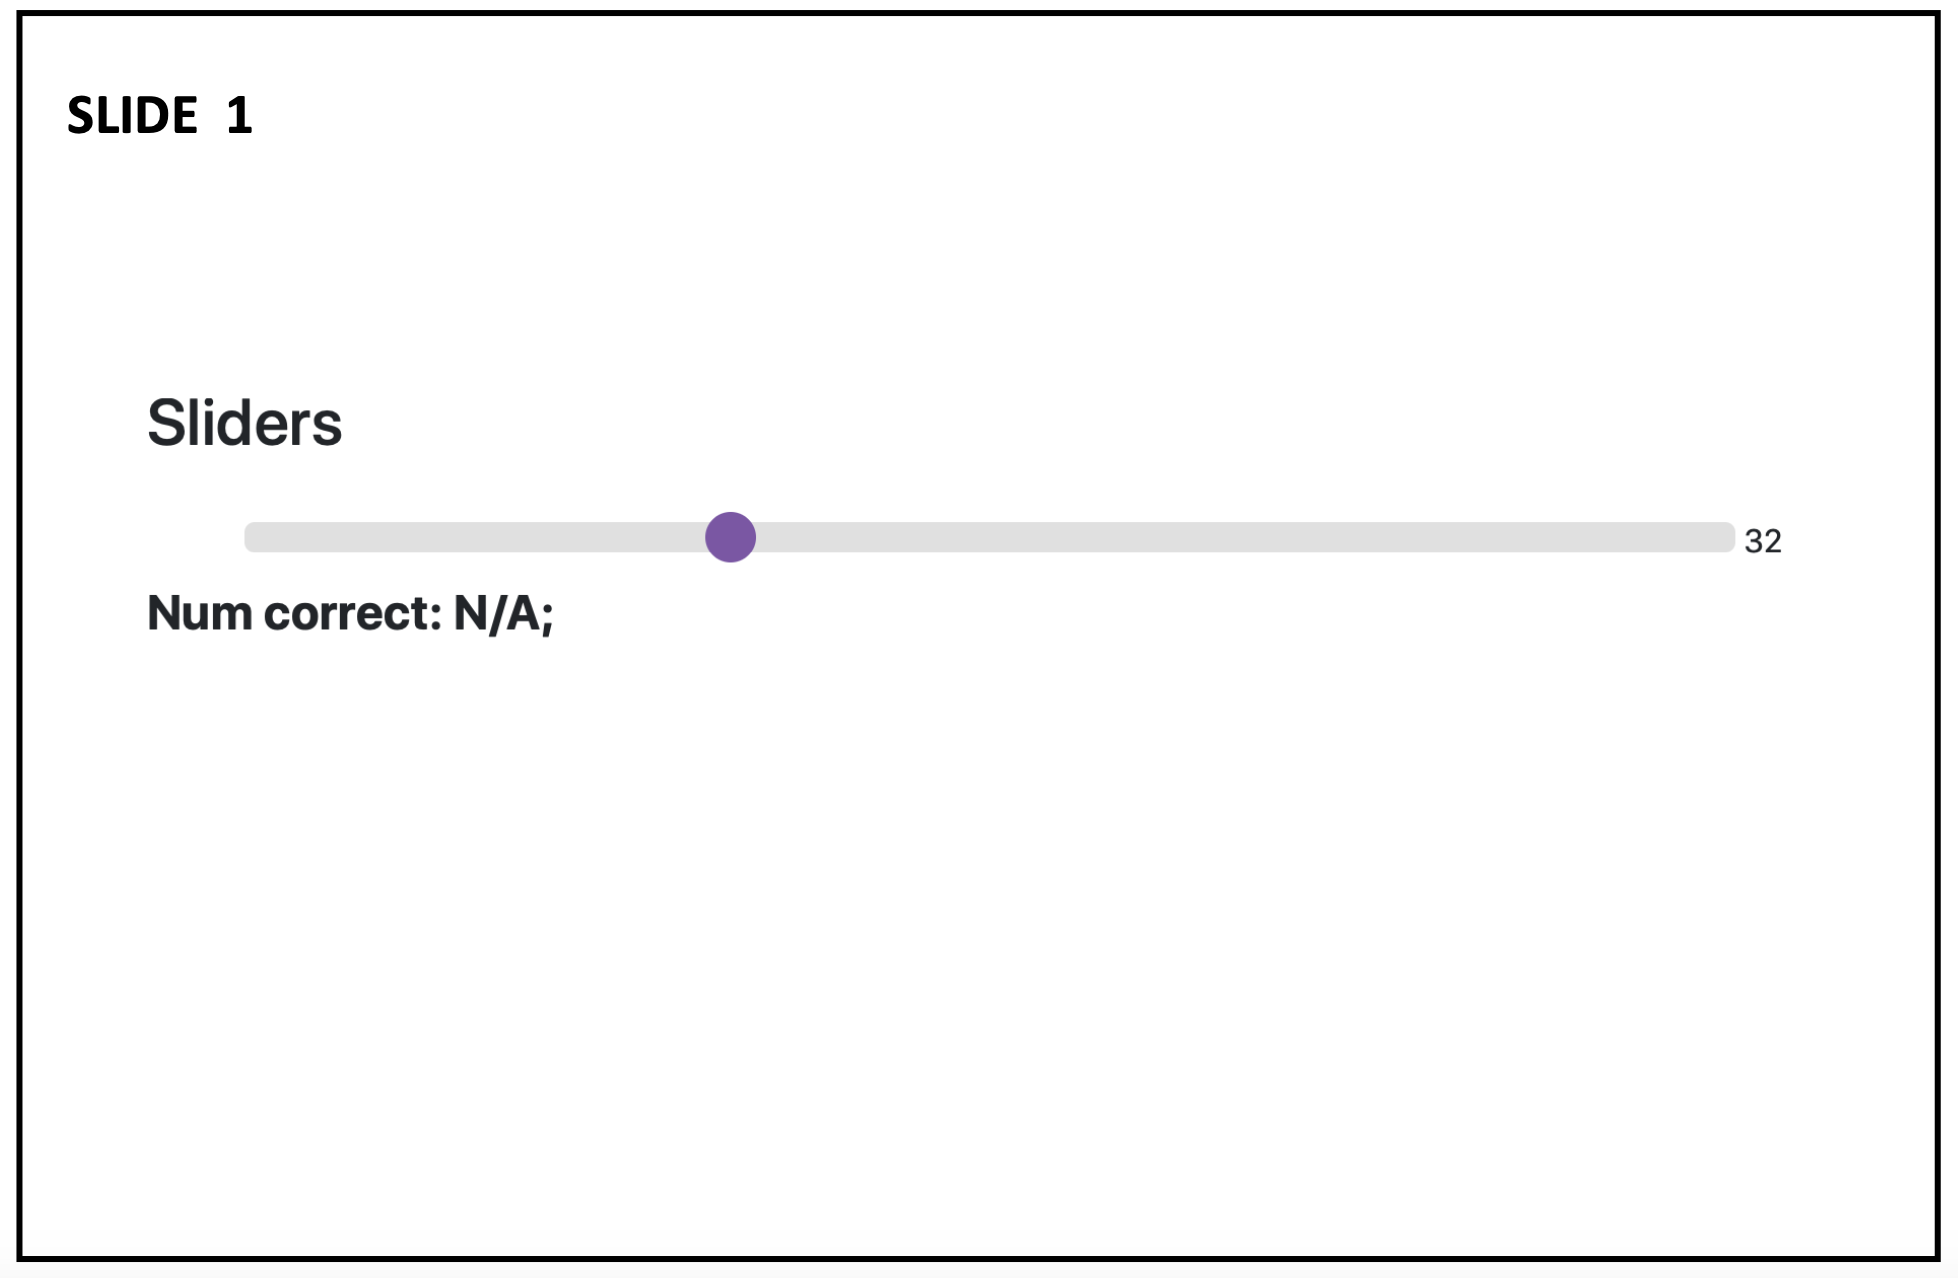
\includegraphics[height=1.7in]{Figs_appA/slide-1.png} \hspace{2mm} 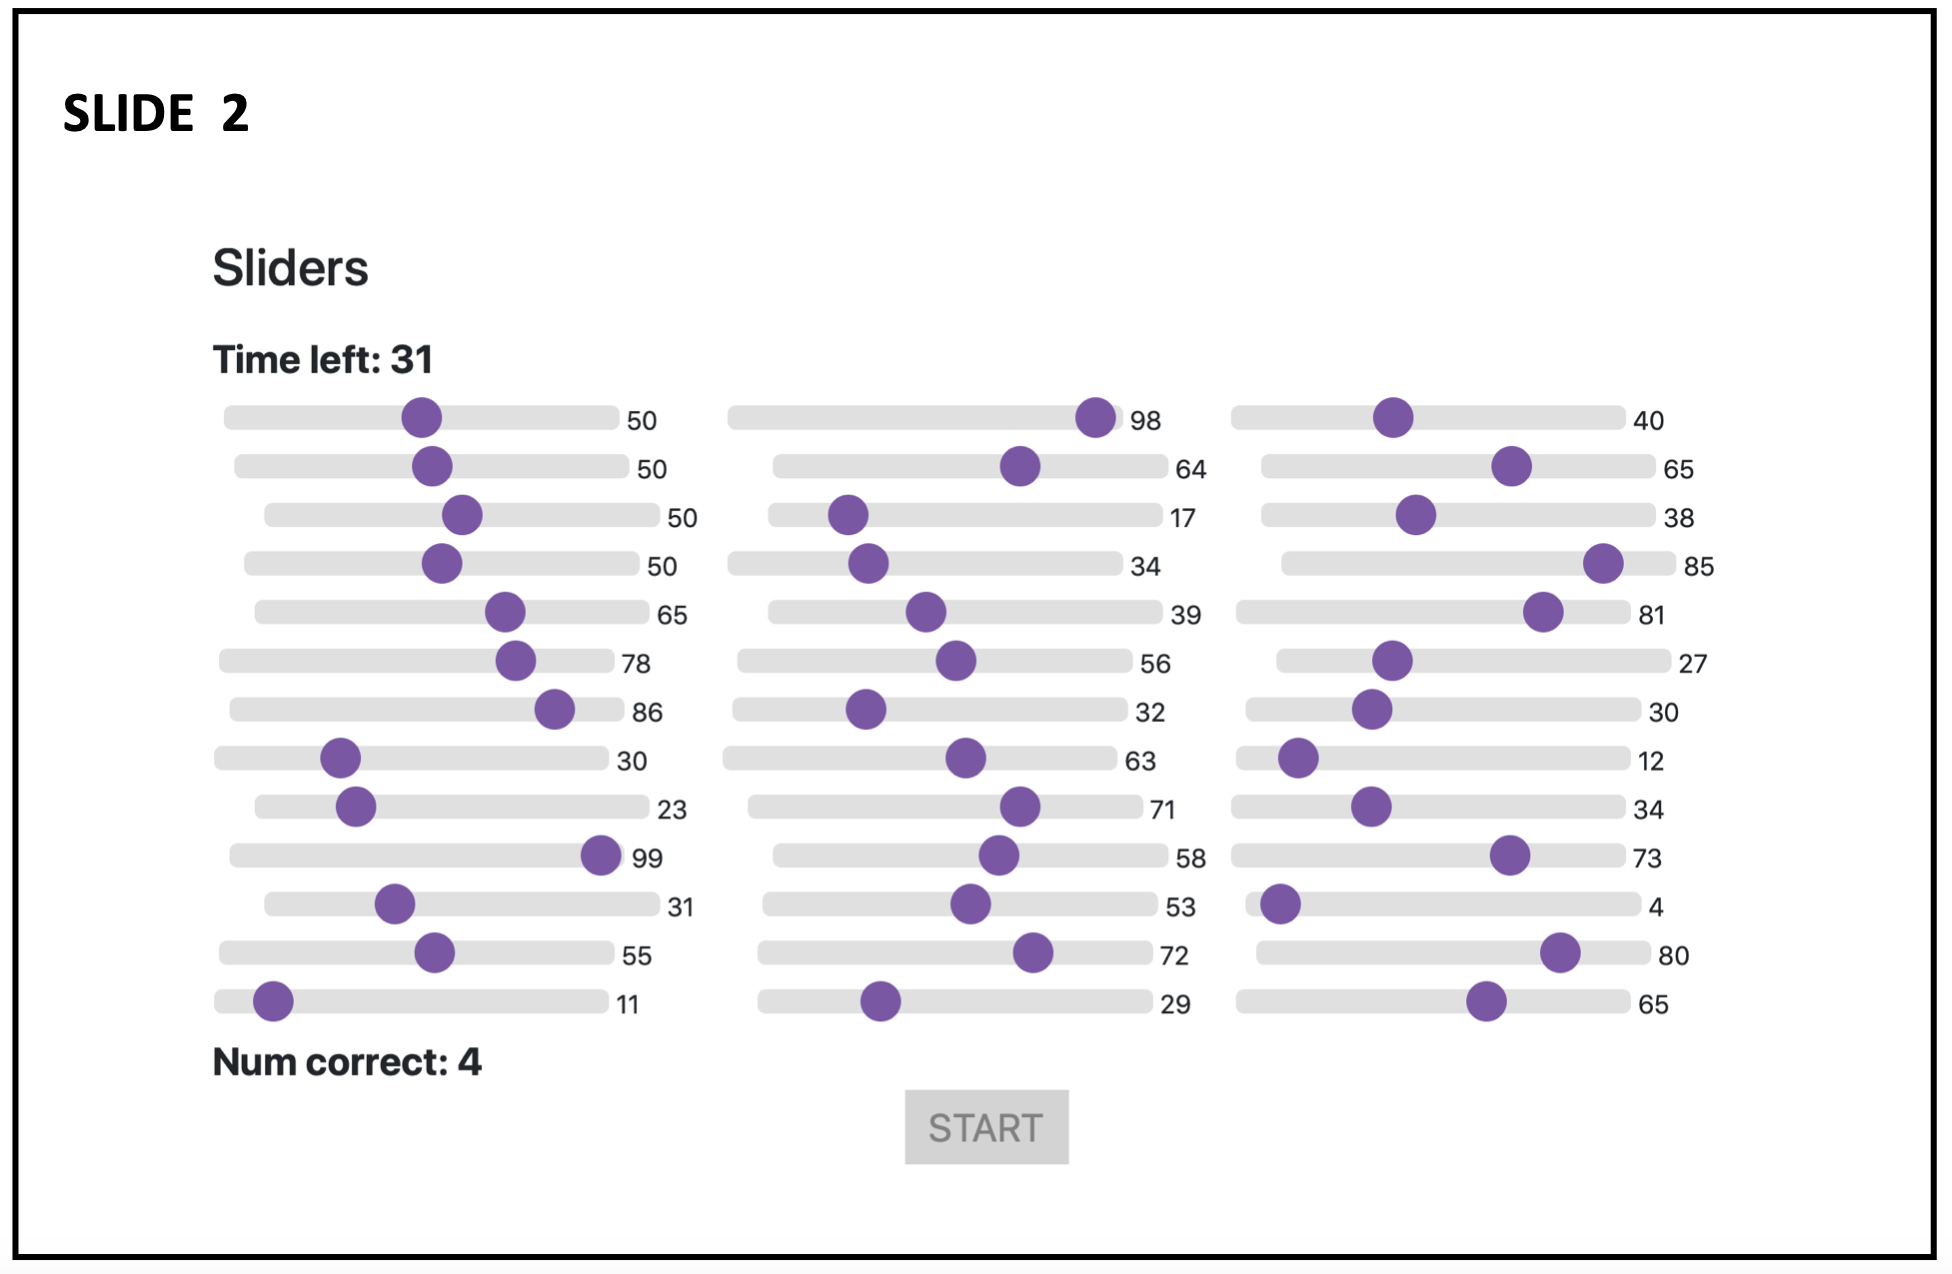
\includegraphics[height=1.7in]{Figs_appA/slide-2.png} \par \vspace*{4mm}
\hspace*{-4mm}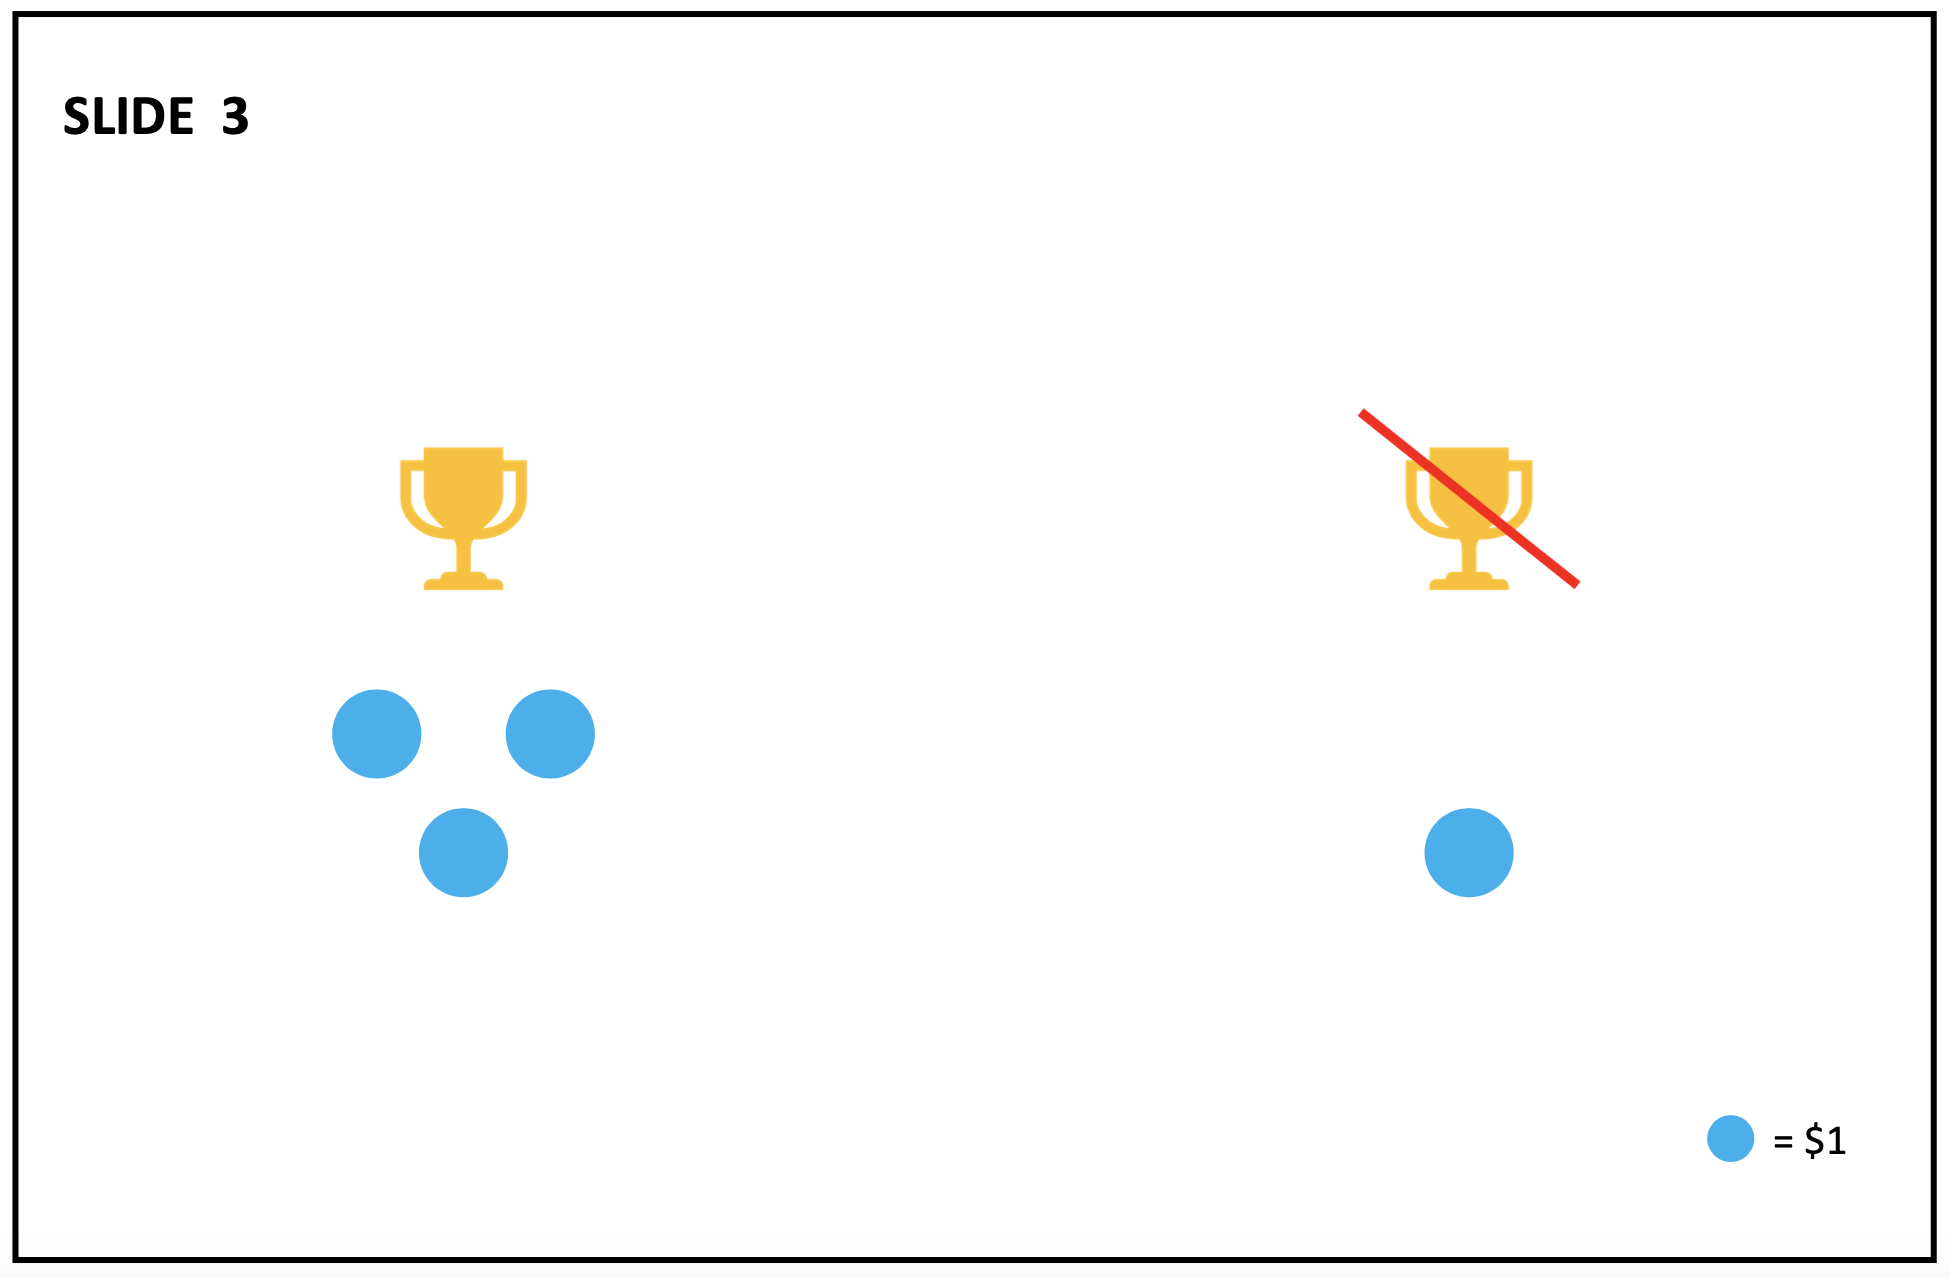
\includegraphics[height=1.7in]{Figs_appA/slide-3.png} \hspace{2mm} 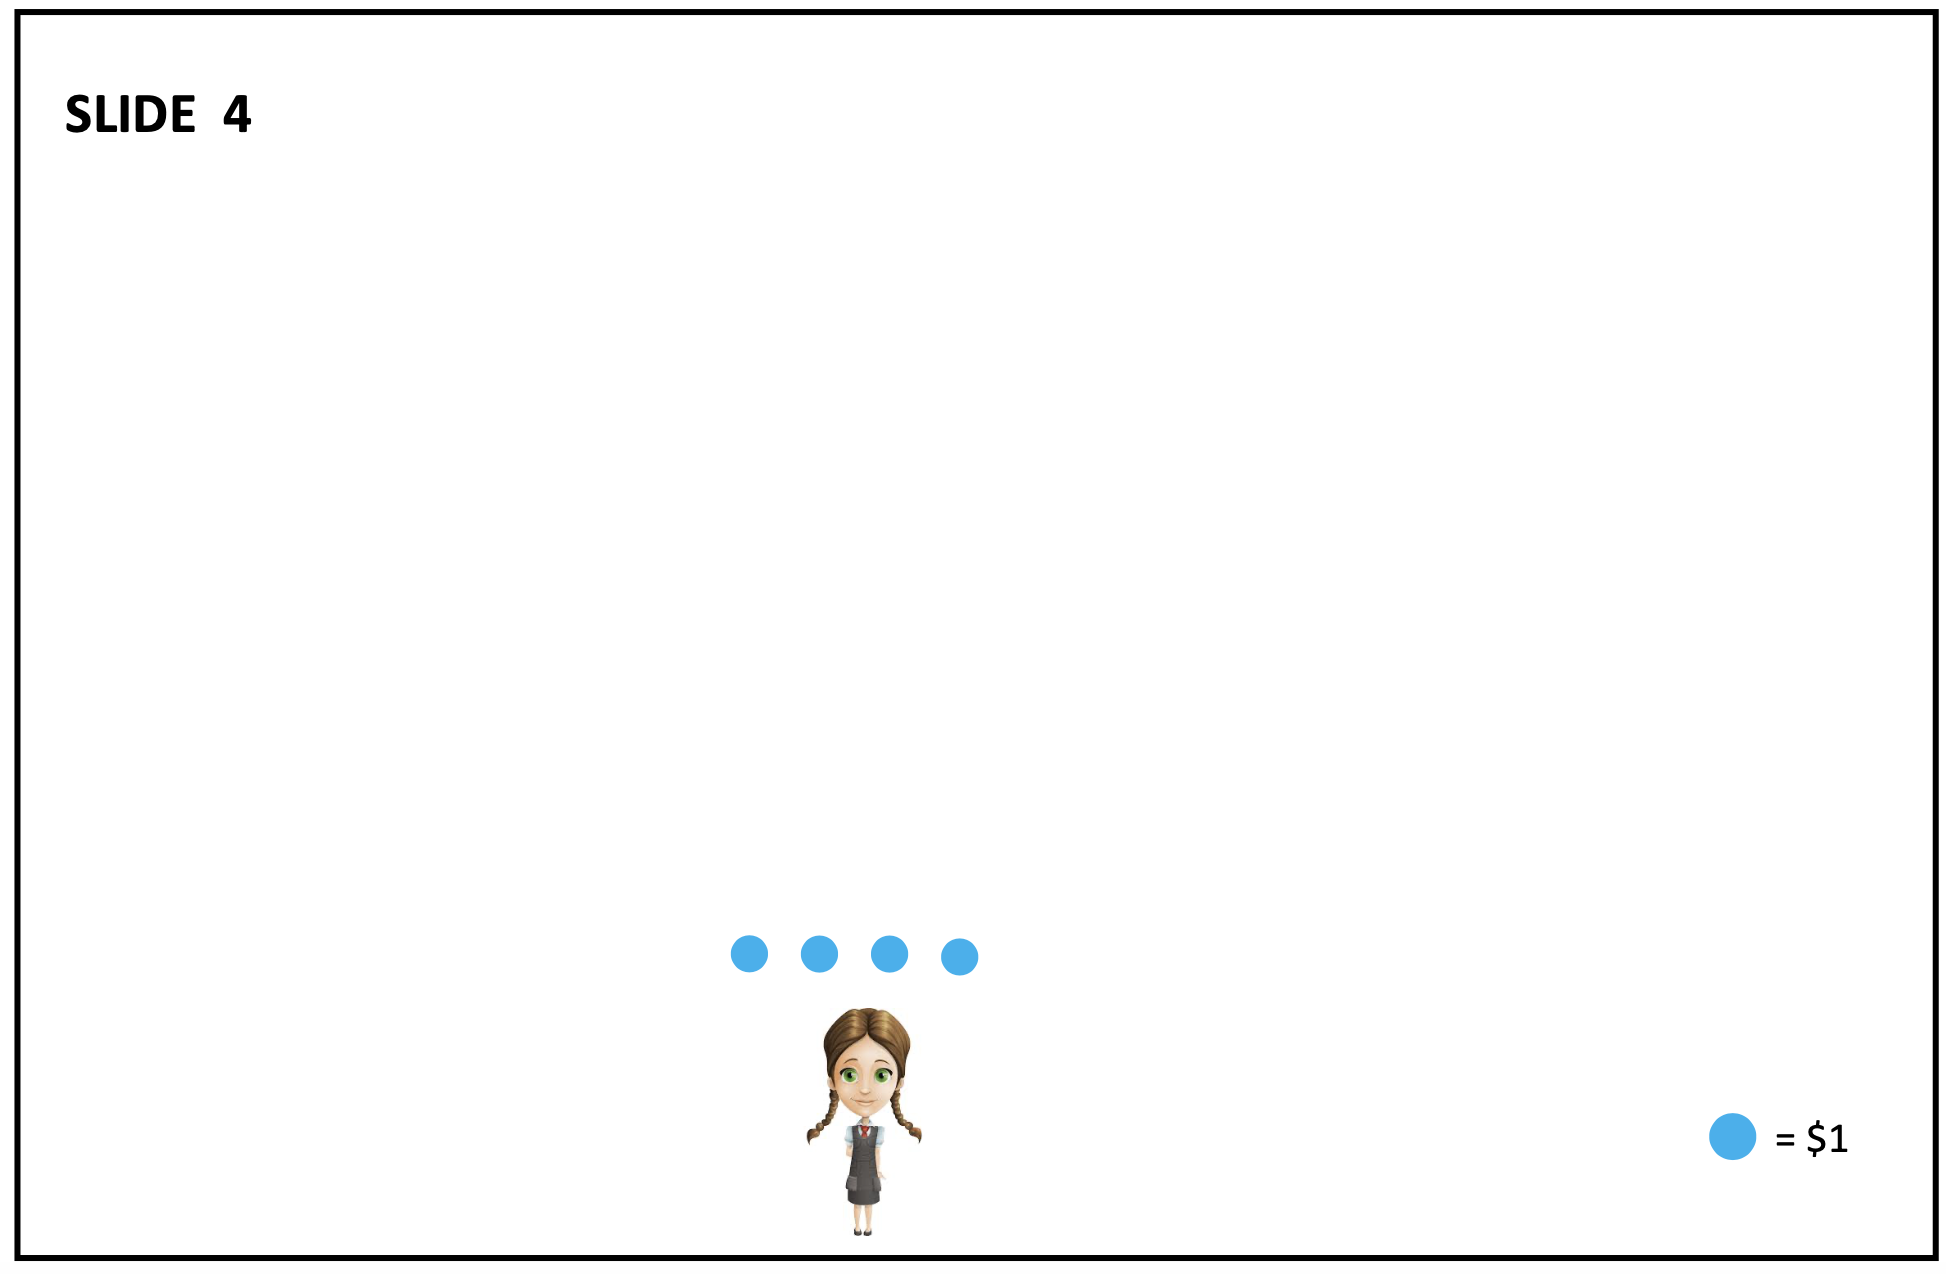
\includegraphics[height=1.7in]{Figs_appA/slide-4.png} \par \vspace*{4mm} 
\hspace*{-4mm}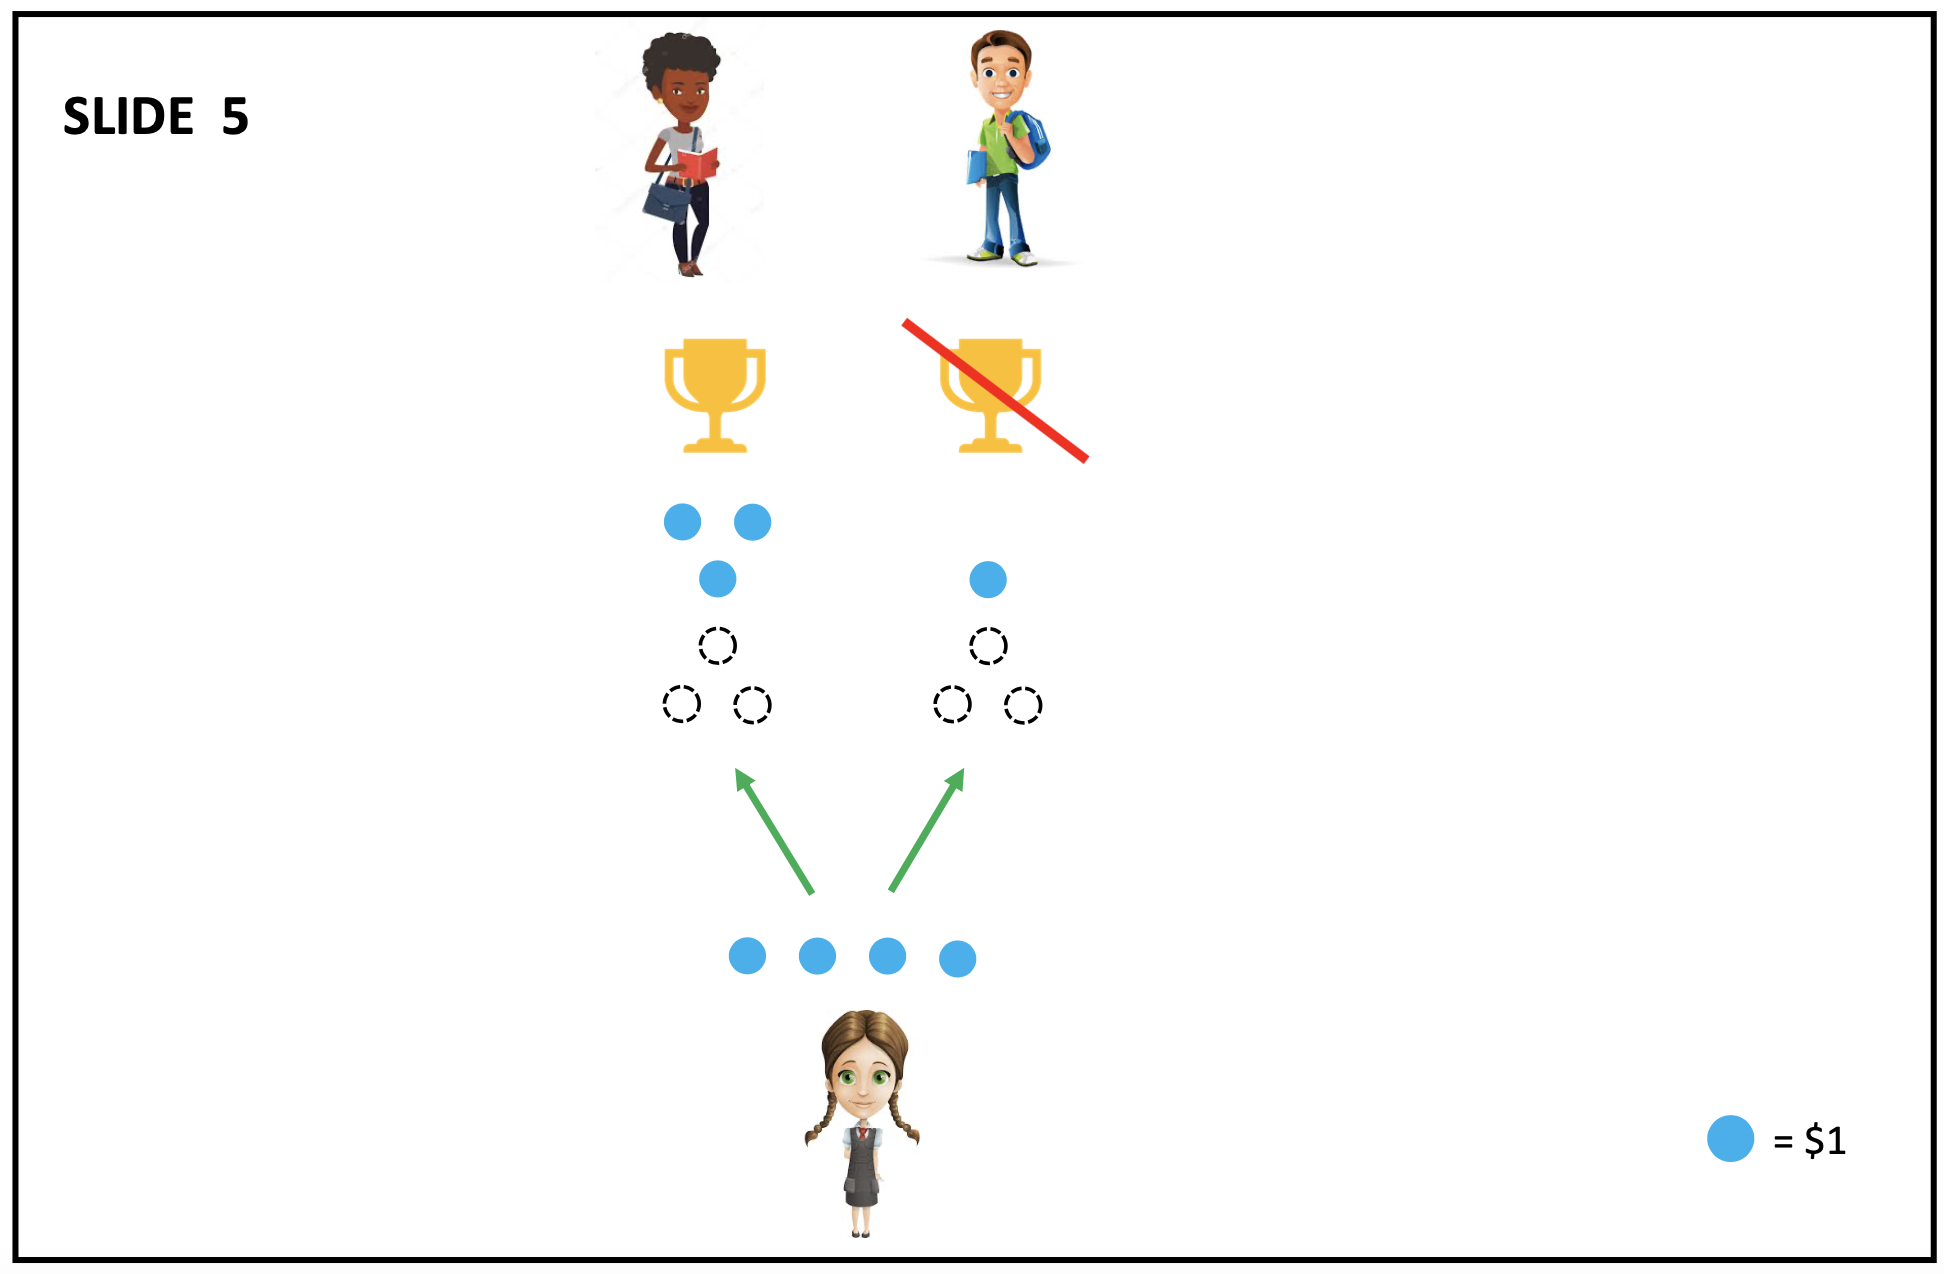
\includegraphics[height=1.7in]{Figs_appA/slide-5.png} \hspace{2mm} 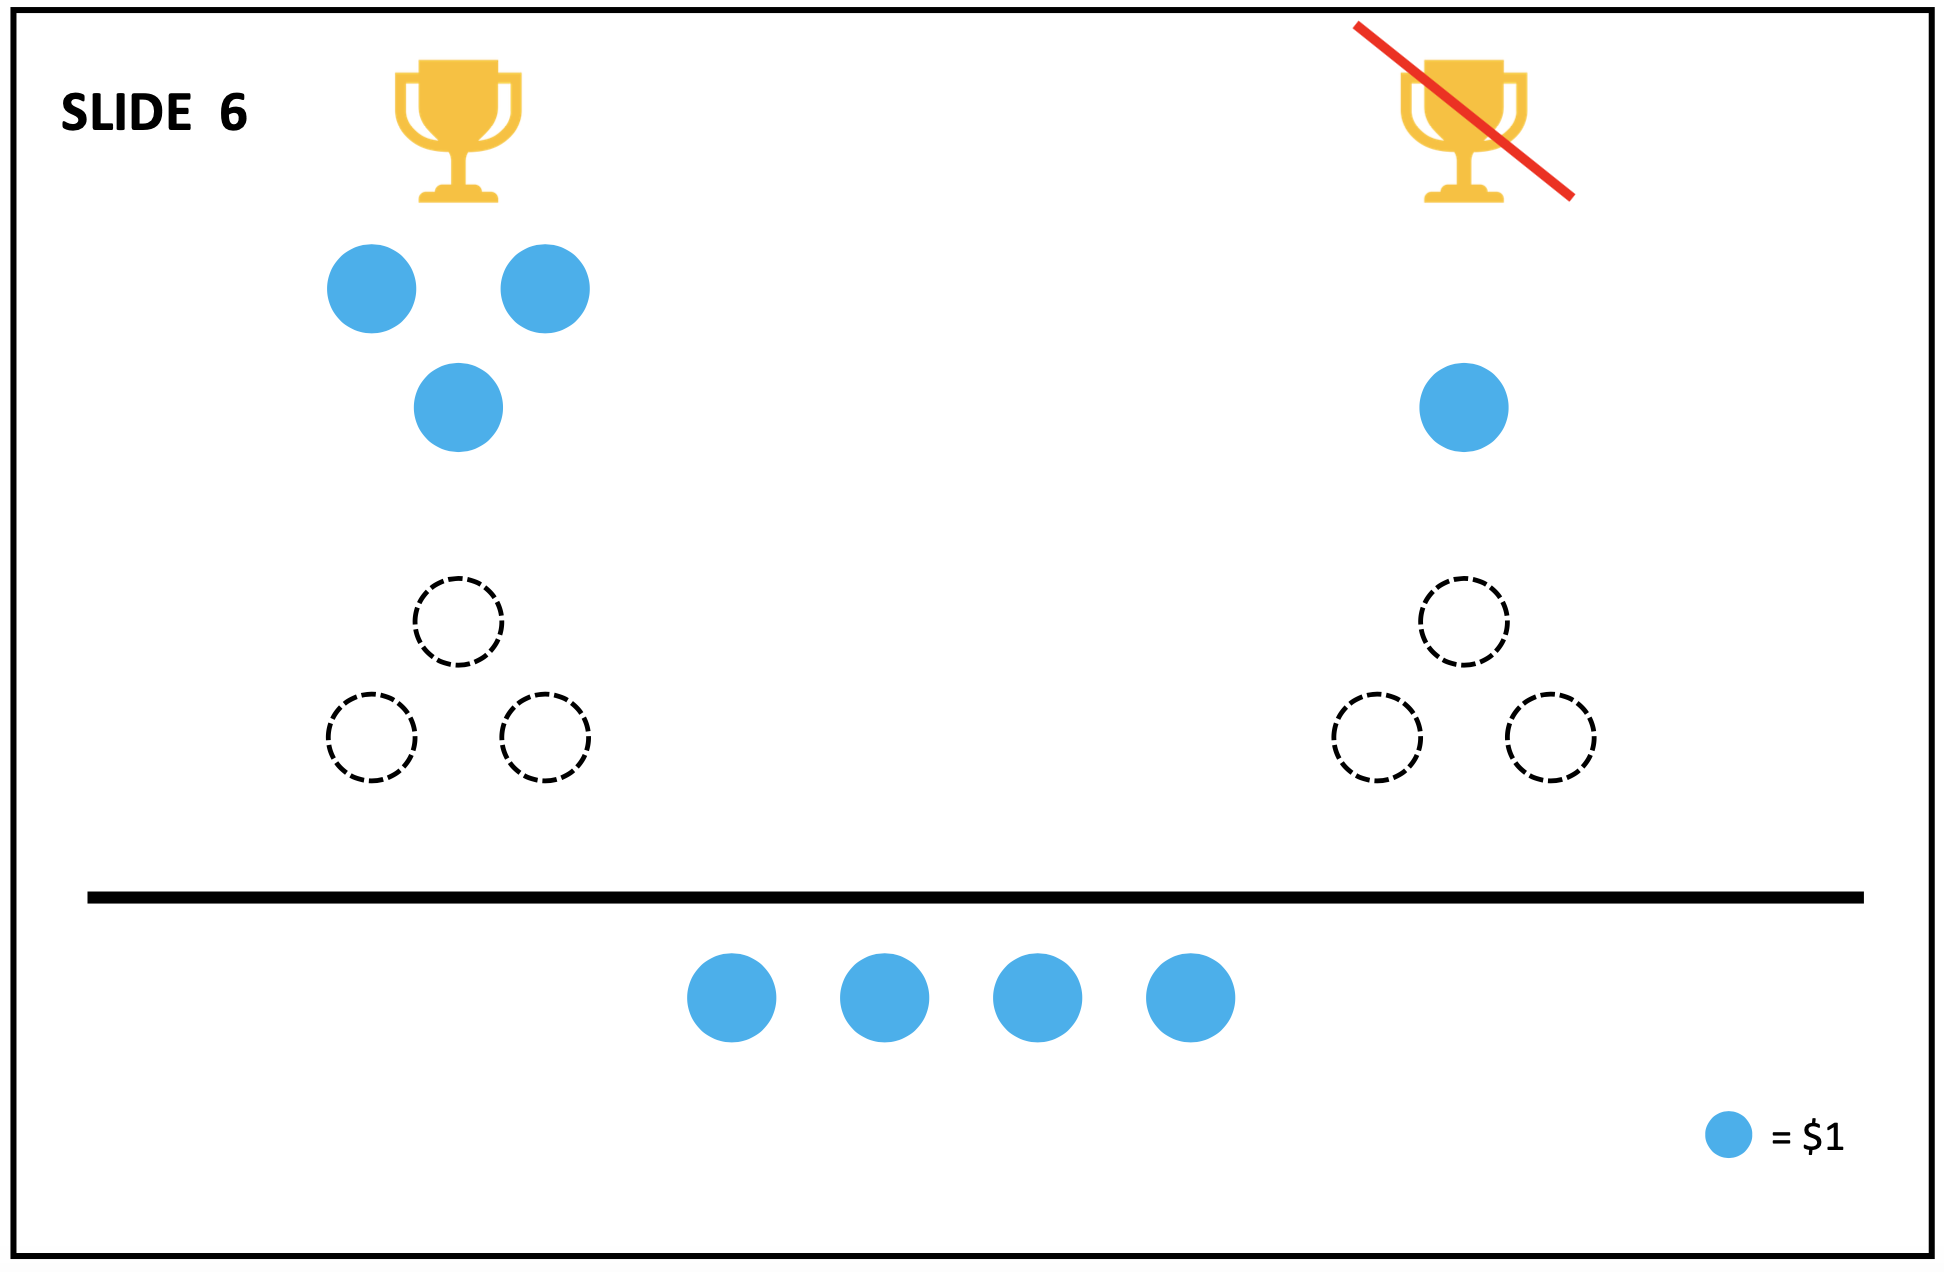
\includegraphics[height=1.7in]{Figs_appA/slide-6.png} \par \vspace*{4mm} 
\hspace*{-4mm}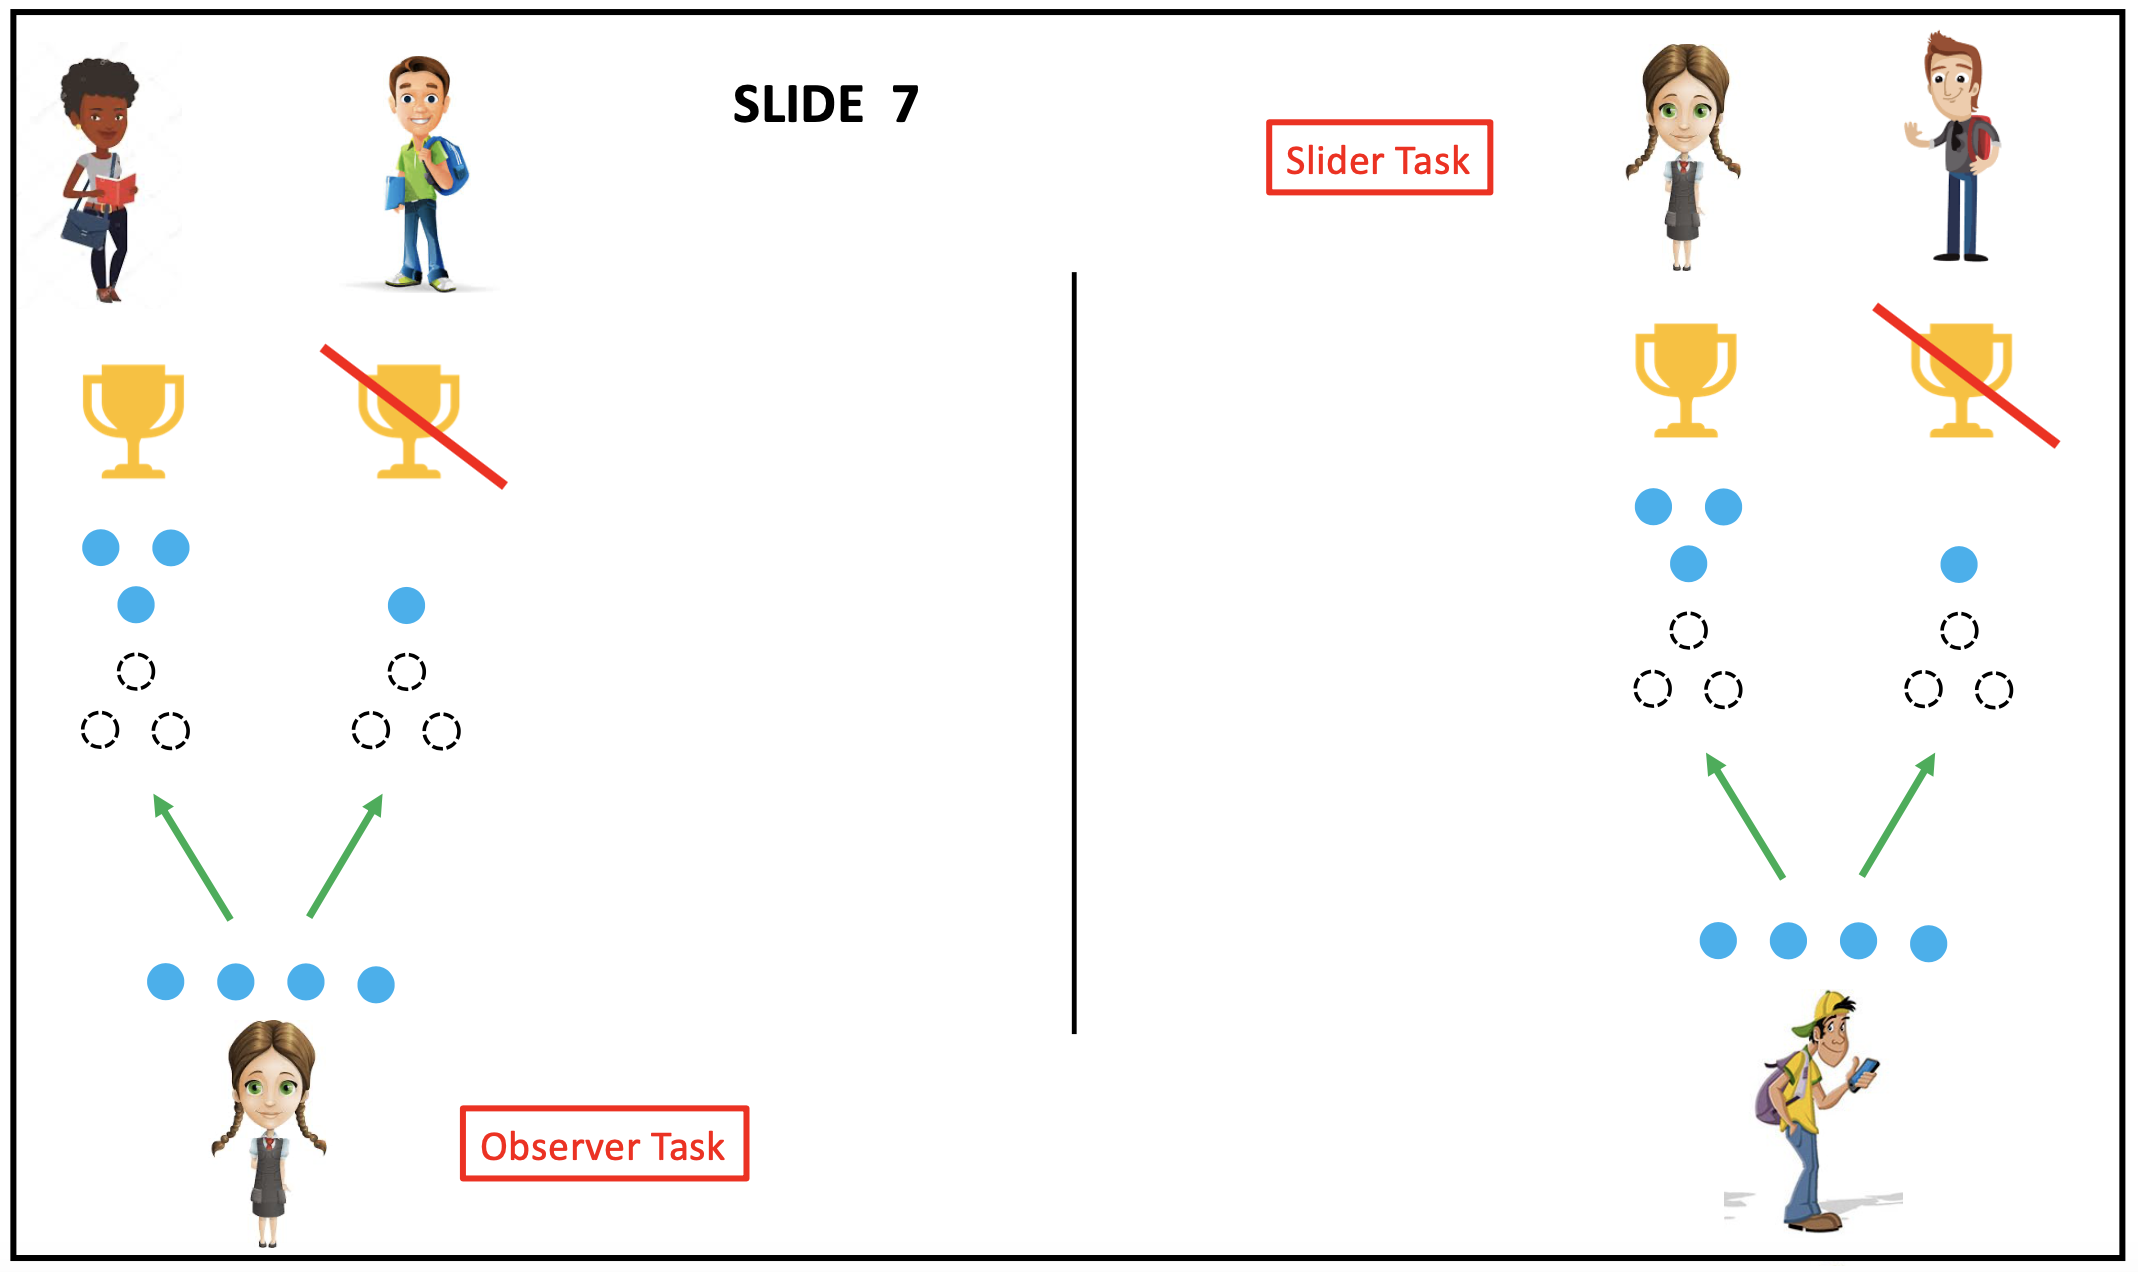
\includegraphics[height=1.7in]{Figs_appA/slide-7.png}  
      	\caption{Slides projected on screen for instructions \label{fig-slides}}
\end{figure} 

\newpage


\noindent {\normalsize {\bf A2. Developmental Read the Mind in the Eyes Test (DeRMET)}} \par \bigskip
	
\noindent \underline{Instructions}. \par \medskip
	

\noindent Below, you will see a series of images with a boy's eyes expressing a certain emotion. Look closely and choose, from the four options, the one that best represents the person's emotion. When you are sure of your answer, press NEXT, and the next image will appear. Once you press NEXT, you will not be able to change your answer. For each correct answer, you will receive 10 points, which is equivalent to 10 cents. The more correct answers, the more money you will earn. \par \bigskip

\noindent  \underline{Note to the instructor}. \par \medskip

\noindent Each image is presented in a different page with four emotions to choose from (see the list below). Participant must select exactly one. After a choice is made, the next image appears on the screen and the participant cannot go back. There is no feedback between images.  \par \bigskip


\noindent  \underline{List of images}. \par \medskip


\begin{figure}[htpb]
\begin{adjustwidth}{}{-17mm} 
\hspace*{-15mm}
1.
\includegraphics[height=0.78in]{Figs_appC/pic1.jpg}\hspace*{3mm}
2.
\includegraphics[height=0.78in]{Figs_appC/pic2.jpg}  \hspace*{3mm}
3.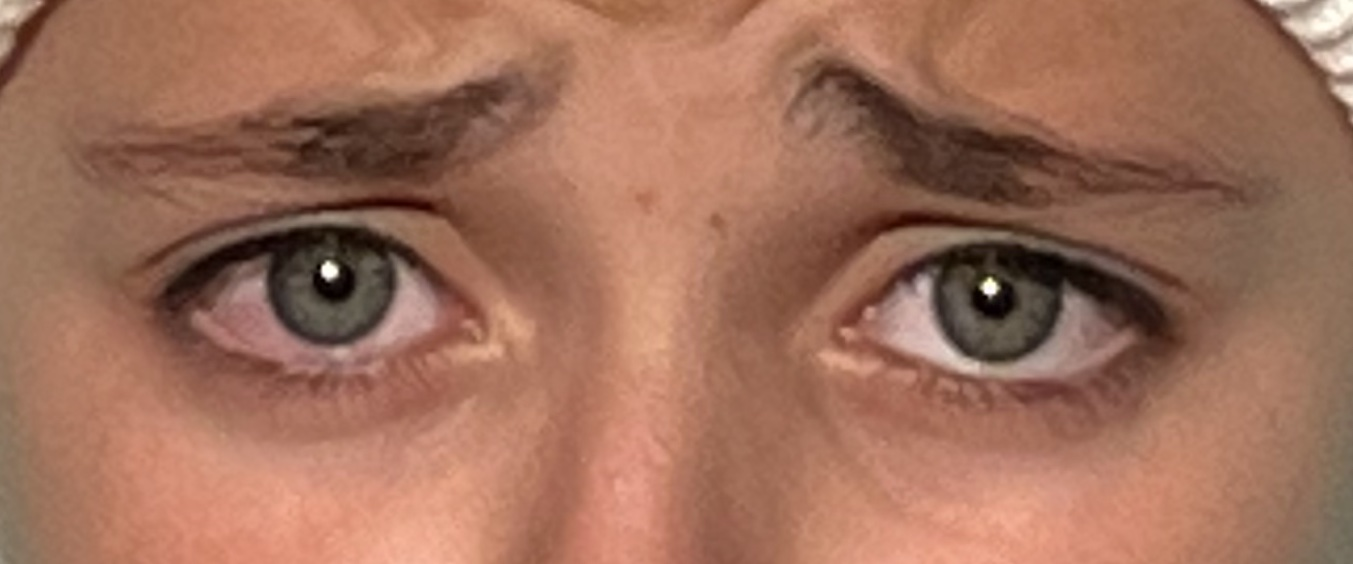
\includegraphics[height=0.78in]{Figs_appC/pic3.jpg} \par\vspace*{4mm}
\hspace*{-20mm}
4.
\includegraphics[height=0.78in]{Figs_appC/pic4.jpg}  \hspace*{3mm}
5.
\includegraphics[height=0.78in]{Figs_appC/pic5.jpg}  \hspace*{3mm}
6.
\includegraphics[height=0.78in]{Figs_appC/pic6.jpg} \par\vspace*{4mm}
\hspace*{-4mm}
7.
\includegraphics[height=0.78in]{Figs_appC/pic7.jpg}  \hspace*{3mm}
8.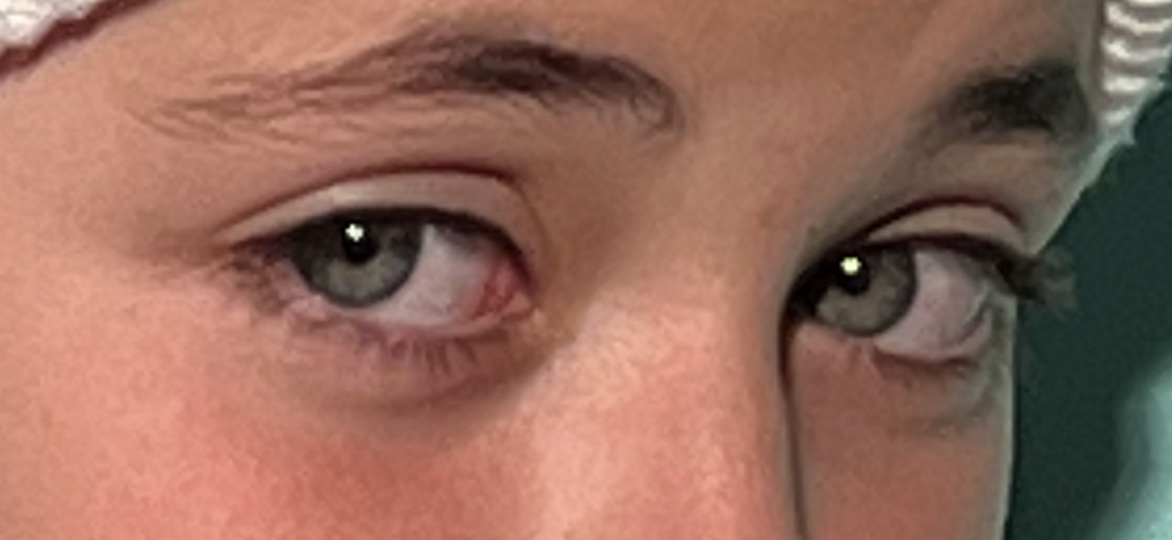
\includegraphics[height=0.78in]{Figs_appC/pic8.jpg}  \hspace*{3mm}
9.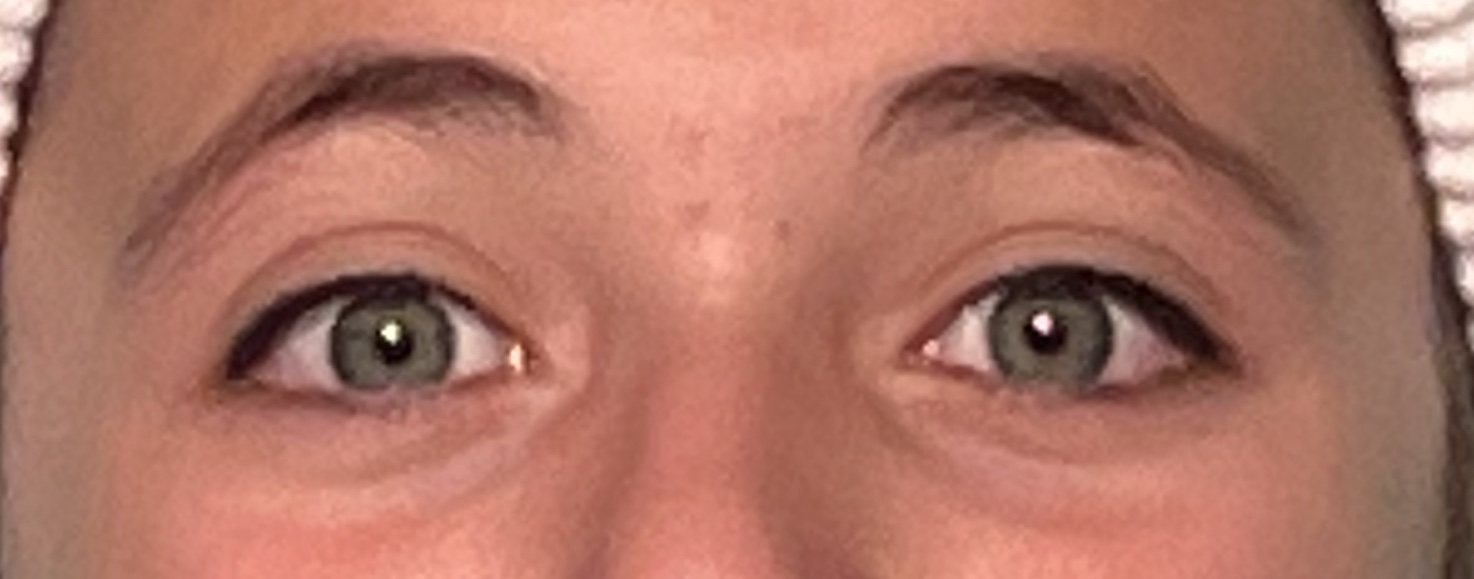
\includegraphics[height=0.78in]{Figs_appC/pic9.jpg} \par\vspace*{4mm}
\hspace*{-15mm}
10.
\includegraphics[height=0.78in]{Figs_appC/pic10.jpg}  \hspace*{3mm}
11.
\includegraphics[height=0.78in]{Figs_appC/pic11.jpg}  \hspace*{3mm}
12.
\includegraphics[height=0.78in]{Figs_appC/pic12.jpg} \par\vspace*{5mm}
\end{adjustwidth}
\end{figure} 


\begin{figure}[htpb]
\begin{adjustwidth}{}{-17mm} 
\hspace*{-15mm}
13.
\includegraphics[height=0.78in]{Figs_appC/pic13.jpg}  \hspace*{3mm}
14.
\includegraphics[height=0.78in]{Figs_appC/pic14.jpg}  \hspace*{3mm}
15.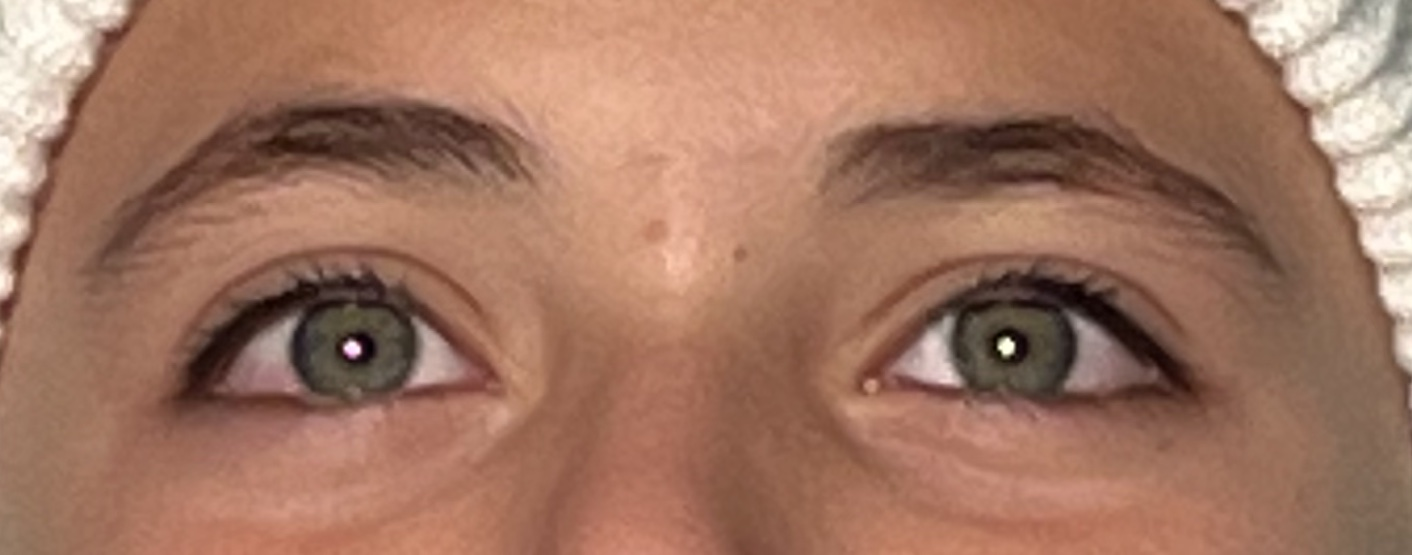
\includegraphics[height=0.78in]{Figs_appC/pic15.jpg} \par\vspace*{4mm}
\centerline{16.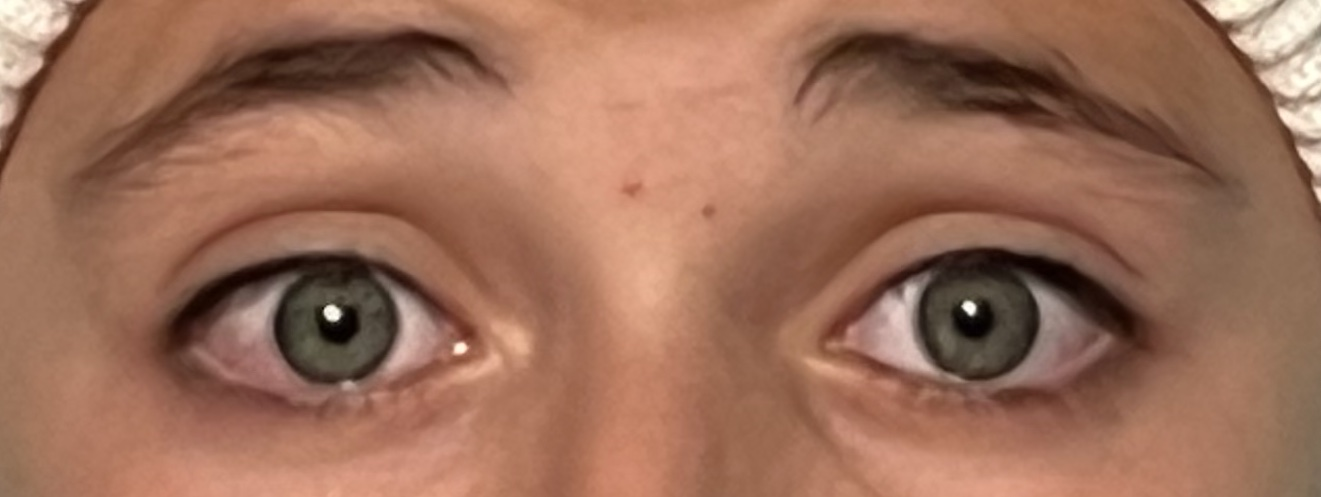
\includegraphics[height=0.78in]{Figs_appC/pic16.jpg}}   
\end{adjustwidth}
\end{figure} 
 


\begin{table}[htpb] 
\small
\begin{flushleft}
\noindent \underline{List of emotions for each image}. \par \medskip

\end{flushleft}

\begin{tabular}{lllllc}  
Image \#  & \multicolumn{4}{c}{Emotions} & \% correct\\  \midrule 
1 & 1. Bored & 2. Confused$^*$ &3. Hopeful & 4. Guilty	& 55.7 \\
2 & 1. Sneaky & 2. Angry & 3. Guilty & 4. Tired$^*$ 	& 79.5\\
3 & 1. Guilty & 2. Tired & 3. Confused & 4. Sad$^*$ 	& 64.5\\
4 & 1. Admiring & 2. Disapproving$^*$ & 3. Shocked & 4. Bored 	& 46.2 \\
5 & 1. Surprised & 2. Admiring & 3. Happy$^*$ & 4. Sneaky 	& 74.3\\
6 & 1. Confused & 2. Ashamed$^*$ & 3. Scared & 4. Tired 	& 69.7 \\
7 & 1. Angry$^*$ & 2. Scared & 3. Sad & 4. Worried 	& 97.2 \\
8 & 1. Excited & 2. Confused & 3. Thinking & 4. Flirting$^*$ & 68.1\\
9 & 1. Excited$^*$ & 2. Happy & 3. Hopeful & 4. Flirting & 75.5\\
10 & 1. Disgusted & 2. Sad & 3. Angry & 4. Scared$^*$ & 88.2\\
11 & 1. Scared & 2. Bored & 3. Disgusted$^*$ & 4. Angry & 70.2\\
12 & 1. Surprised & 2. Happy & 3. Thinking$^*$ & 4. Disapproving  & 86.6\\
13 & 1. Hopeful & 2. Sneaky$^*$ & 3. Thinking & 4. Excited	& 89.4 \\
14 & 1. Guilty & 2. Bored & 3. Disgusted & 4. Worried$^*$ 	& 59.7 \\ 
15 & 1. Happy & 2. Surprised & 3. Hopeful$^*$ & 4. Sneaky & 46.2 \\
16 & 1. Surprised$^*$ & 2. Happy & 3. Flirting & 4. Admiring & 66.8\\ \midrule
\multicolumn{6}{l}{\footnotesize [$^*$ = correct answer. The last column reports for each image the aggregate empirical probability of} \\ 
\multicolumn{6}{l}{\footnotesize  finding the correct answer]}
\end{tabular} 
\end{table}  
 
 
\pagebreak 



\noindent {\normalsize {\bf A3. Pictorial Big 5 personality questionnaire}} \par \bigskip
	
\noindent \underline{Instructions}. \par \medskip

Next, you will see a series of pictures. The group of pictures on the left represents one type of behavior, while the group of pictures on the right represents the opposite type of behavior. Look at the pictures in each group and choose the option that best represents you. \par \medskip

For example, imagine you saw this screen \par \medskip


\begin{figure}[htpb]
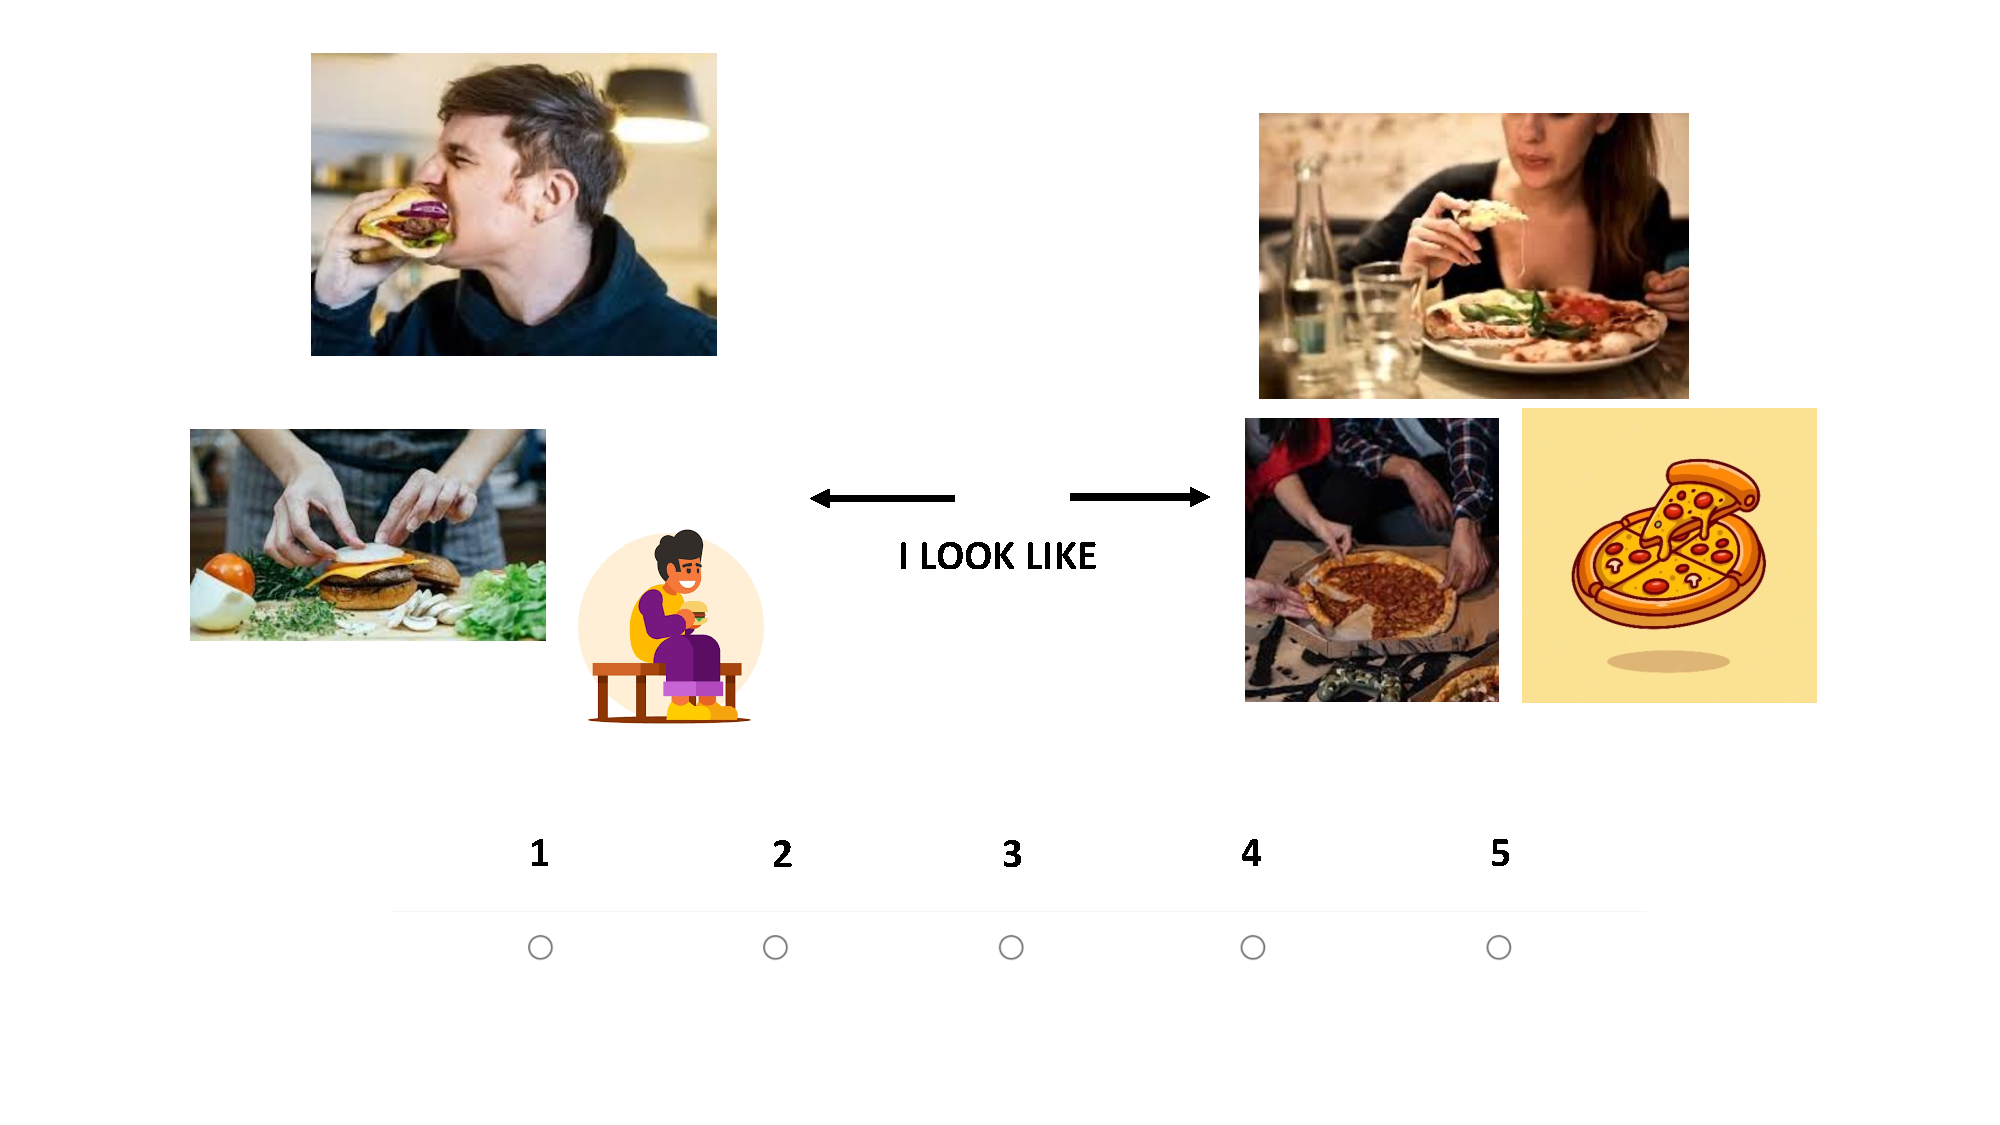
\includegraphics[height=2in]{Figs_appC/burgerpizza.pdf}  

\end{figure} 

\newpage

We would be asking if you definitely prefer hamburgers (1), mostly hamburgers (2), both equally (3), mostly pizza (4) or definitely pizza (5). The questions are about your character or behavior. When you are sure, press NEXT, and another series of pictures will appear. There are no right or wrong answers, and please remember that your responses are confidential. \par \bigskip
	
\noindent \underline{Questionnaire}. \par \medskip

\noindent The groups of pictures presented to our participants are provided below. They correspond to the following traits: extraversion (1), agreeableness (2), conscientiousness (3), neuroticism (4) and openness (5).

\begin{figure}[htpb]
\begin{adjustwidth}{}{-10mm} 
\hspace*{-2mm}
1.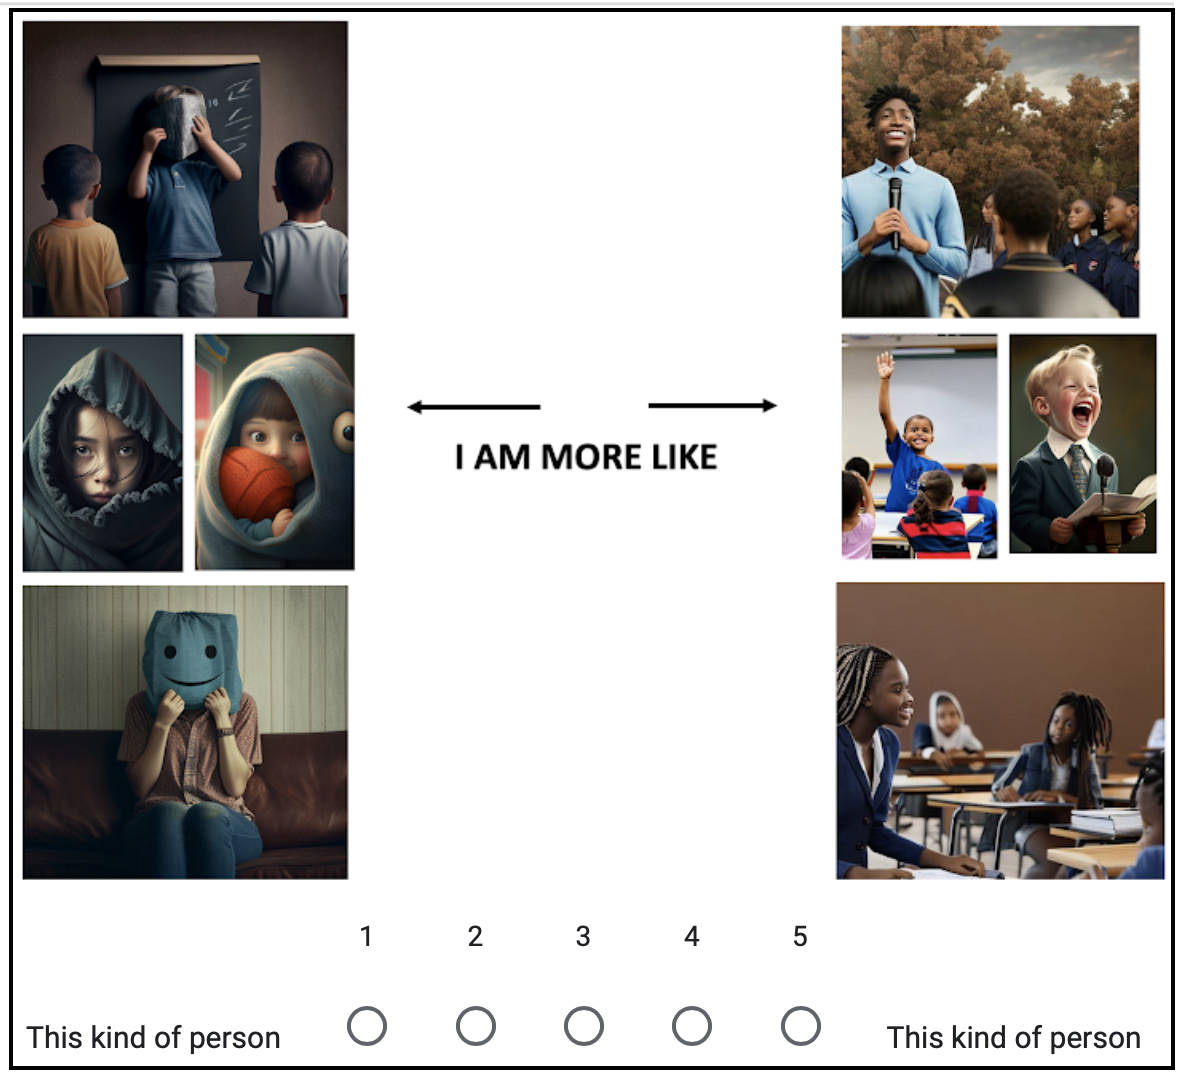
\includegraphics[height=2.4in]{Figs_appC/personality1.png}  \hspace*{3mm}
2.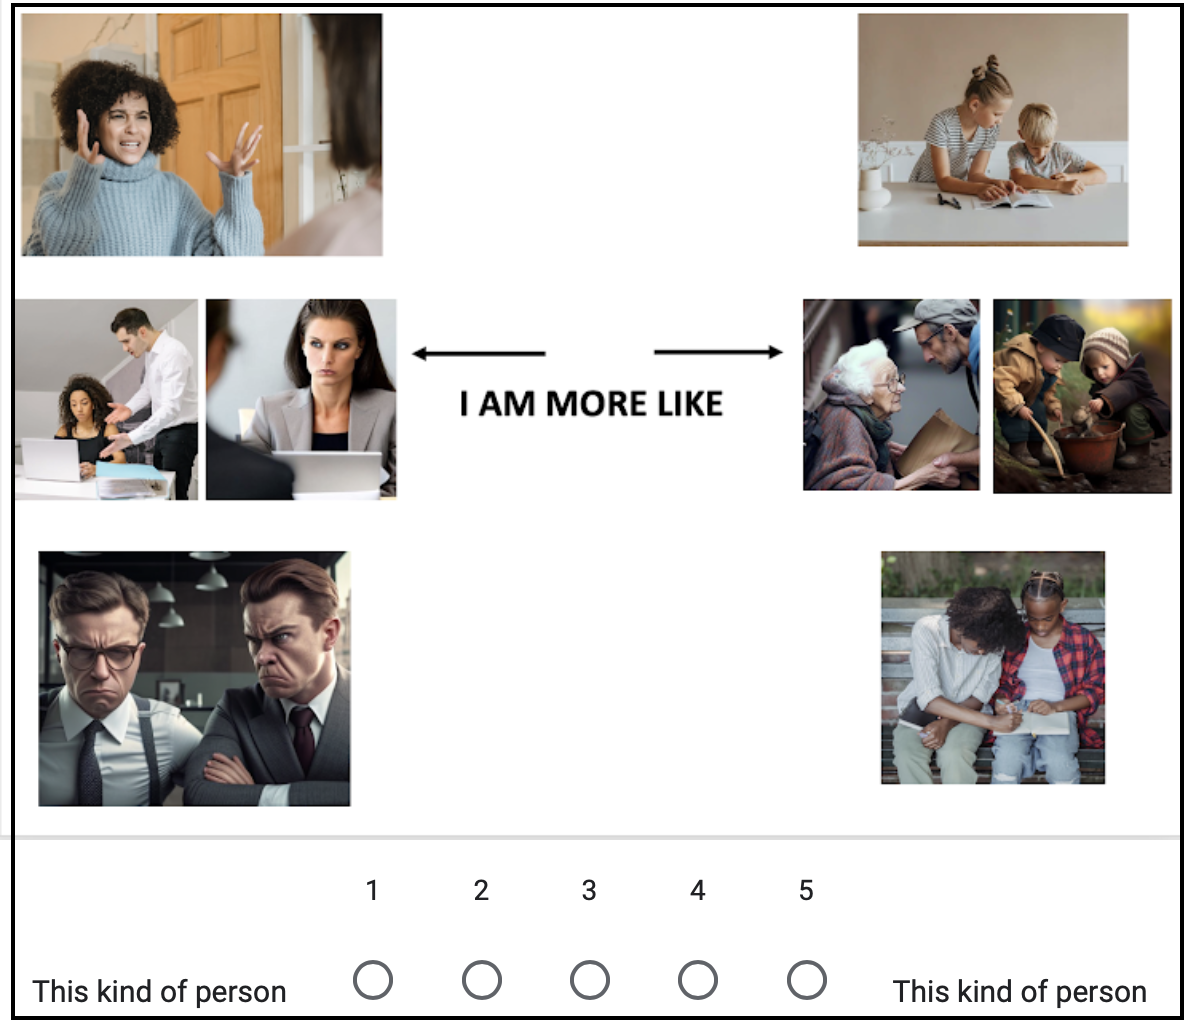
\includegraphics[height=2.4in]{Figs_appC/personality2.png}  
\end{adjustwidth}
\end{figure} 

\begin{figure}[htpb]
\begin{adjustwidth}{}{-10mm} 
\hspace*{-2mm}
3.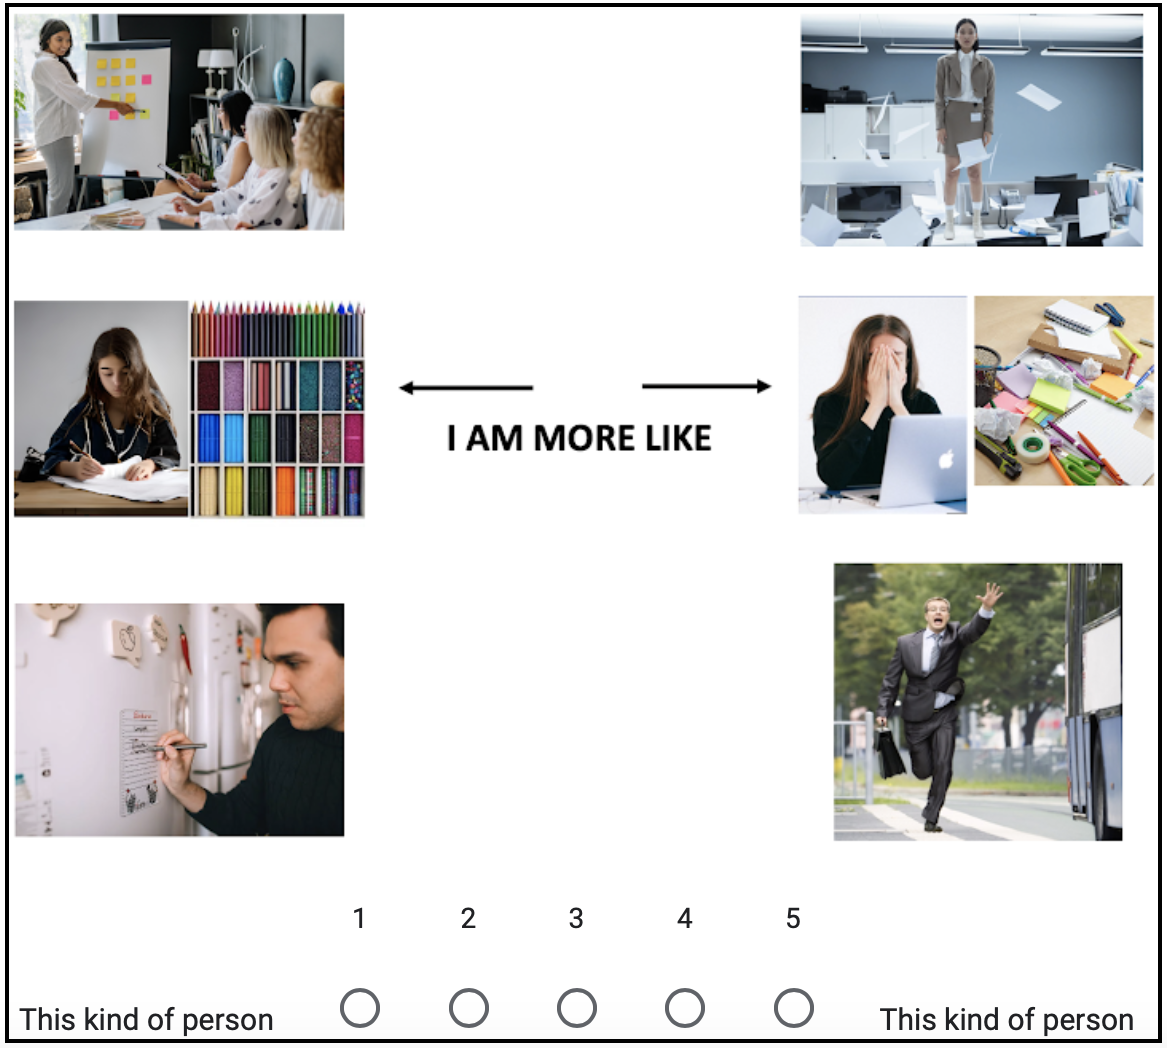
\includegraphics[height=2.4in]{Figs_appC/personality3.png} \hspace*{3mm}
%
4.\includegraphics[height=2.4in]{Figs_appC/personality4.png}\par \vspace*{6mm}
\centerline{5.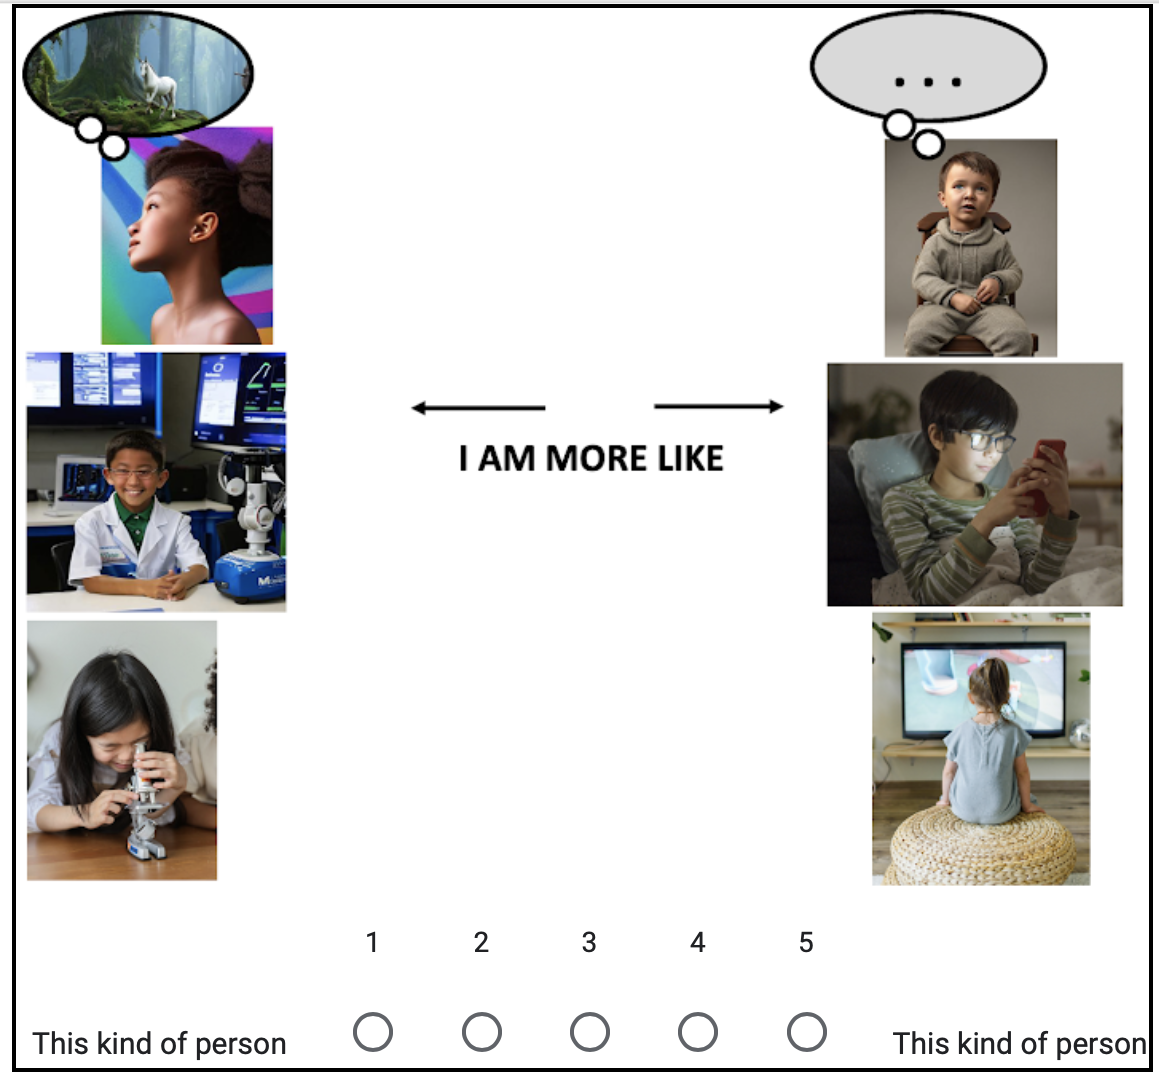
\includegraphics[height=2.5in]{Figs_appC/personality5.png}}   
\end{adjustwidth}
\end{figure} 

 
\clearpage

\centerline{\large {\bf Appendix B. Additional Analyses}} \par \vspace*{6mm}

\noindent {\normalsize {\bf B1. Descriptive statistics for the variables of interest}}\par \medskip

\noindent For the descriptive analysis, we cluster students in age-groups according to the Spanish school system: early elementary (US grades 1, 2 and 3), late elementary (US grades 4, 5 and 6), early middle school (US grades 7 and 8), late middle school (US grades 9 and 10) and high school (US grades 11 and 12). Descriptive statistics of the individual characteristics and performance in the tasks are summarized in \autoref{tab:summary}. 

% latex table generated in R 4.4.2 by xtable 1.8-4 package
% Thu Oct 15 18:03:41 2026
\begin{table}[ht]
\centering
\begin{tabular}{rlllll}
  \hline
 & Early Elem. & Late Elem. & Early Middle & Late Middle & High School \\ 
  \hline
\% Male & 47.33 & 54.62 & 54.03 & 52.87 & 55.7 \\ 
  \% Siblings & 78.42 & 88.87 & 84.07 & 88.28 & 86.32 \\ 
  \% STEM & 40.37 & 39.55 & 37.5 & 47.82 & 57 \\ 
  Pay Winner Before & 5.08 (0.82) & 5.03 (0.76) & 5.05 (0.76) & 5 (0.75) & 5.04 (0.74) \\ 
  Pay Winner After & 5.02 (0.84) & 4.97 (0.72) & 4.88 (0.71) & 4.91 (0.75) & 4.95 (0.71) \\ 
  ScoreTom & 9.12 (2.5) & 11.03 (2.43) & 12.1 (2.06) & 12.56 (1.97) & 12.64 (1.75) \\ 
  Extraversion & 3.63 (1.39) & 3.74 (1.08) & 3.65 (1.05) & 3.6 (0.95) & 3.5 (0.95) \\ 
  Agreeableness & 4.19 (1.17) & 4.09 (1.03) & 3.88 (0.94) & 3.87 (0.87) & 3.9 (0.89) \\ 
  Conscientiousness & 4.08 (1.24) & 3.63 (1.27) & 3.31 (1.23) & 3.03 (1.19) & 3.24 (1.19) \\ 
  Neuroticism & 1.6 (1.04) & 1.7 (0.96) & 1.89 (0.92) & 2.03 (0.91) & 2.13 (0.93) \\ 
  Openness & 3.44 (1.54) & 3.13 (1.29) & 2.87 (1.14) & 2.83 (1.09) & 2.97 (1.05) \\ 
   \hline
\end{tabular}
\caption{Summary Statistics by Age Group - mean (standard deviation)} 
\label{tab:summary}
\end{table}


All five groups have a sufficient number of observations and are well-balanced in terms of gender. A good exogenous measure is the percentage of children who have at least one sibling. It appears to be very similar across age groups, with the only difference being in the youngest group (which is precisely the most likely group to increase that number). 

Performance in DeRMET rises steeply between early and late elementary school, more slowly through middle school, and is nearly flat between late middle school and high school (see Appendix B7 for further details). Patterns in the Pictorial Big depend on the trait: agreeableness, conscientiousness and openness decrease with age, neuroticism increases and extraversion remains roughly constant. It is particularly interesting that in most cases, the variables reach their peak (or minimum) in late middle school (see Appendix B6 for further details). \par \bigskip

\noindent {\normalsize {\bf B2. Gender effects}} \par \medskip



\input{Figs/Table9.tex} 


\autoref{regtreatmentGender} reports a further analysis of gender effects by interacting gender with Environment and Condition variables. Male participants allocate less to the loser: the male coefficient is negative and statistically significant for the initial allocation, while the corresponding effect in the final allocation is negative but not statistically different from zero. Task effects are generally small on average, but the interaction patterns indicate heterogeneity: in the initial decision, the \emph{talent} condition is substantially less equalizing than the omitted baseline in the \emph{addition} environment, while under \emph{redistribution} the talent effect is more favorable to the loser ($Redistribution \times Talent$ is positive and significant). In the final decision, there is evidence that males respond differently to the \emph{effort} condition: $Effort \times Male$ is negative and statistically significant, implying a larger reduction in the loser’s allocation among males in the effort condition, while the remaining two-way and three-way interactions (including $Redistribution \times Male$ and the triple interactions) are not statistically distinguishable from zero.








\bigskip



\noindent {\normalsize {\bf B3. Replication of the main regressions studying age effects of the \emph{initial} and \emph{final} payoffs of the loser with alternative specifications.}} \par \medskip

We consider different specifications. \autoref{table-b3-initial-class} and \autoref{table-b3-final-class} present the results when we cluster the standard errors at the classroom level only. \autoref{table-b3-initial-both} and \autoref{table-b3-final-both} present the results when we cluster the standard errors at both the classroom and campus levels.

\input{Figs/Table10}

\input{Figs/Table11}

\input{Figs/Table12}

\newpage

\input{Figs/Table13}




\noindent {\normalsize {\bf B4. Replication of the main regressions using age-groups}} \par \medskip
 
\noindent  In \autoref{table-b4-noFE} and \autoref{table-b4-FE}, we replicate the most relevant results of the study using the age-groups described in Appendix B1 instead of the age in months of our participants. We cluster standard errors at the classroom level and we use campus FE in addition in \autoref{table-b4-FE} (as in the main text).

\begingroup
\let\JPEoriginaltable\table
\def\table[#1]{\JPEoriginaltable[htpb]}
\input{Figs/Table14.tex}
\endgroup





\par \medskip

The first and second columns study the initial decisions of participants. In \emph{redistribution} (column 1), the early-middle-school coefficient is associated with more meritocratic allocations, especially among boys. This corresponds to the slight, imprecisely estimated curvature in \autoref{table-age-initial}. In \emph{addition} (column 2), coefficients are positive for both early and late middle schoolers, with the largest point estimate in early middle school. Overall, the age-group estimates are qualitatively consistent with Result \ref{res-initial}, while the exact shape of the initial profile remains specification-dependent. \par \medskip
 
 

The third and fourth columns examine final decisions. In \emph{redistribution} (column 3), we do not detect an age effect, whereas in \emph{addition} (column 4) the point estimates again describe a concave pattern with a similar peak. Overall, the age-group specifications are qualitatively consistent with the profiles described in Result \ref{res-final}. \par\bigskip

\input{Figs/Table15.tex}



\noindent {\normalsize {\bf B5. Final choices in \emph{redistribution\/} with separate regressions}}  \par \medskip


\noindent \autoref{table-b5} and \autoref{fig-62-separate} present the same analysis of final choices in the \emph{redistribution\/} treatment as \autoref{table-age-final} (columns 1 and 2) and \autoref{superfigure-redist}, except that regressions are performed separately for the three winner selections methods. In the main text, we advocated for one regression with dummy variables to increase statistical power. However, and although results must be taken with a grain of salt, it is still instructive to perform the three separate regressions to check if the age-trajectory is similar across conditions.
 
\begin{table}[htpb]
\centering
\footnotesize
\begin{tabular}{l cc cc cc}
\toprule
 & \multicolumn{2}{c}{\textit{effort}} & \multicolumn{2}{c}{\textit{talent}} & \multicolumn{2}{c}{\textit{luck}} \\
\cmidrule(lr){2-3} \cmidrule(lr){4-5} \cmidrule(lr){6-7}
 & (1) & (2) & (3) & (4) & (5) & (6) \\
\midrule
Age & $-0.008$ & $-0.006$ & $-0.000$ & $0.000$ & $-0.002$ & $-0.002$ \\
        & ($0.012$) & ($0.012$) & ($0.006$) & ($0.006$) & ($0.016$) & ($0.016$) \\
Age$^2$ & $0.00002$ & $0.00002$ & $0.00000$ & $0.00000$ & $0.00001$ & $0.00001$ \\
        & ($0.00004$) & ($0.00004$) & ($0.00002$) & ($0.00002$) & ($0.00005$) & ($0.00005$) \\
Male &  & $-0.191^{*}$ &  & $-0.150^{**}$ &  & $0.023$ \\
        &  & ($0.100$) &  & ($0.066$) &  & ($0.102$) \\
Siblings &  & $0.013$ &  & $0.006$ &  & $-0.075$ \\
        &  & ($0.093$) &  & ($0.117$) &  & ($0.092$) \\
STEM &  & $0.007$ &  & $0.109$ &  & $-0.033$ \\
        &  & ($0.078$) &  & ($0.095$) &  & ($0.098$) \\
\midrule
Obs. & 383 & 383 & 333 & 333 & 362 & 362 \\
Adj. R$^2$ & -0.001 & 0.006 & -0.003 & 0.003 & -0.000 & -0.007 \\
\bottomrule
\multicolumn{7}{l}{\footnotesize $^{***}p<0.01$; $^{**}p<0.05$; $^{*}p<0.1$. SE clustered at the session level.}
\end{tabular}
\caption{OLS regressions of \textit{final} allocation in the \textit{redistribution} treatment, performed separately on each winner selection method}
\label{table-b5}
\end{table}

 

 \begin{figure}[H]
 \small
%\vspace*{-20mm}
\captionsetup{font=small} 
\noindent \hspace*{-8mm}  
   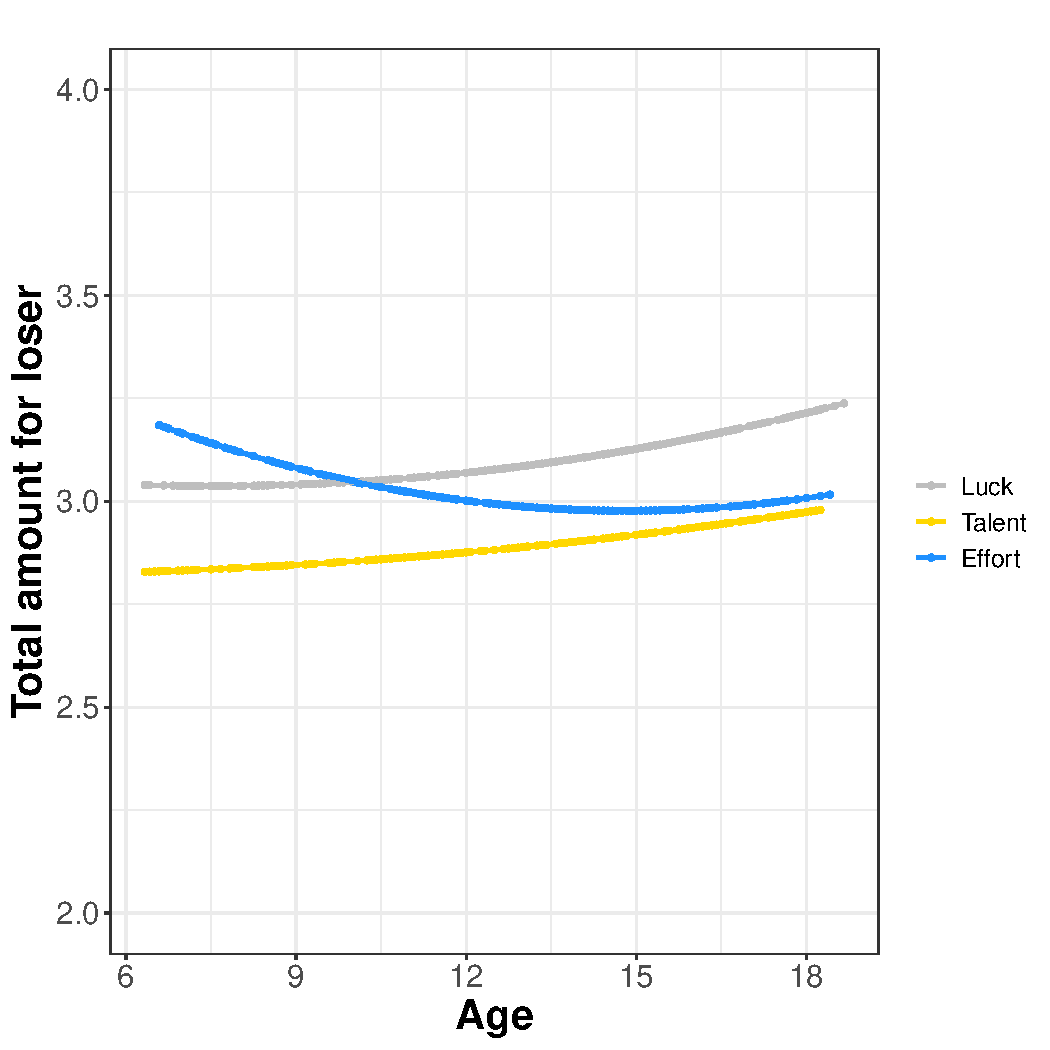
\includegraphics[width=2.5in]{Figs/figure9.pdf} 
 \caption{Smoothed display of fitted age profiles from separate quadratic regressions in \emph{final\/} allocation in the \emph{redistribution\/} treatment, performed separately on each winner selection method} \label{regression-redistribution-separate} \label{fig-62-separate} 
\end{figure}

The age trajectory (or rather lack of) is similar when regressions are performed separately. Perhaps the most noticeable difference is the surprising result that our youngest participants (age 9 and below) tend to redistribute less to the loser in luck than in effort. Interestingly, the documented tendency of males to choose more meritocratic allocations remains in place for effort and talent while it disappears when winners are chosen randomly. \par\bigskip


\noindent {\normalsize {\bf B6. Final choices in  \emph{addition\/}  with separate regressions}} \par \medskip

\noindent \autoref{table-b6} and \autoref{fig-31-separate} present the same analysis of final choices in the \emph{addition\/} treatment as \autoref{table-age-final} (columns 3 and 4) and \autoref{superfigure-addit}, again with regressions performed on each of the three winner selections methods in order to check the age-trajectory separately for each case.
 
\begin{table}[htpb]
\centering
\footnotesize
\begin{tabular}{l cc cc cc}
\toprule
 & \multicolumn{2}{c}{\textit{effort}} & \multicolumn{2}{c}{\textit{talent}} & \multicolumn{2}{c}{\textit{luck}} \\
\cmidrule(lr){2-3} \cmidrule(lr){4-5} \cmidrule(lr){6-7}
 & (1) & (2) & (3) & (4) & (5) & (6) \\
\midrule
Age & $0.019$ & $0.020$ & $0.013$ & $0.015$ & $0.034^{***}$ & $0.033^{***}$ \\
        & ($0.015$) & ($0.014$) & ($0.013$) & ($0.013$) & ($0.009$) & ($0.009$) \\
Age$^2$ & $-0.00007$ & $-0.00007$ & $-0.00004$ & $-0.00004$ & $-0.00010^{***}$ & $-0.00010^{***}$ \\
        & ($0.00005$) & ($0.00005$) & ($0.00004$) & ($0.00004$) & ($0.00003$) & ($0.00003$) \\
Male &  & $-0.324^{***}$ &  & $-0.188^{**}$ &  & $-0.154^{*}$ \\
        &  & ($0.049$) &  & ($0.072$) &  & ($0.083$) \\
Siblings &  & $-0.077$ &  & $-0.042$ &  & $-0.056$ \\
        &  & ($0.137$) &  & ($0.102$) &  & ($0.090$) \\
STEM &  & $-0.037$ &  & $-0.043$ &  & $0.056$ \\
        &  & ($0.084$) &  & ($0.064$) &  & ($0.069$) \\
\midrule
Obs. & 330 & 330 & 382 & 382 & 439 & 439 \\
Adj. R$^2$ & 0.009 & 0.052 & 0.006 & 0.018 & 0.077 & 0.082 \\
\bottomrule
\multicolumn{7}{l}{\footnotesize $^{***}p<0.01$; $^{**}p<0.05$; $^{*}p<0.1$. SE clustered at the session level.}
\end{tabular}
\caption{OLS regressions of \textit{final} allocation in the \textit{addition} treatment, performed separately on each winner selection method}
\label{table-b6}
\end{table}


\begin{figure}[H]
\small
\vspace*{-2mm}
\captionsetup{font=small} 
\noindent \hspace*{-8mm}  
  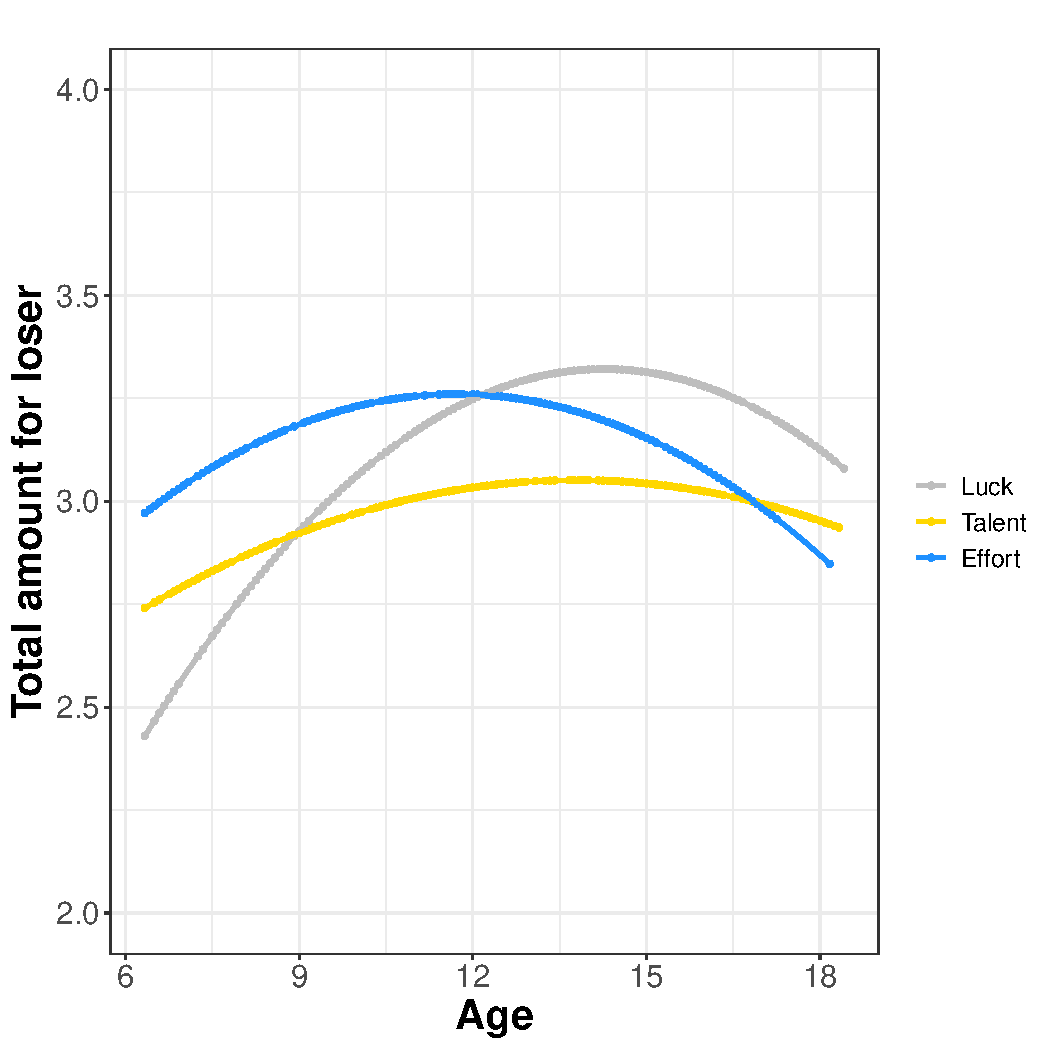
\includegraphics[width=2.5in]{Figs/figure10.pdf} 
 \caption{Smoothed display of fitted age profiles from separate quadratic regressions in \emph{final\/} allocation in the \emph{addition\/} treatment, performed separately on each winner selection method} \label{regression-addition-separate} \label{fig-31-separate} 
\end{figure}

Again, the point estimates are qualitatively similar when regressions are performed separately, supporting the concave age profile of allocation to the loser in \emph{addition}. Finer grade-by-condition comparisons are less precise and should be interpreted cautiously. Males are estimated to be more meritocratic across the winner-selection methods. \par \bigskip
 



\noindent {\normalsize {\bf B7. Developmental RMET (DeRMET)}}\par \medskip


\noindent{\bf a. Performance}\par \medskip

\noindent \autoref{fig-noncog} (left) summarizes the distribution of the number of correct answers in the DeRMET task by grade, with the grade average displayed at the top.

%\begin{figure}[htpb]
%\vspace*{-10mm}
%	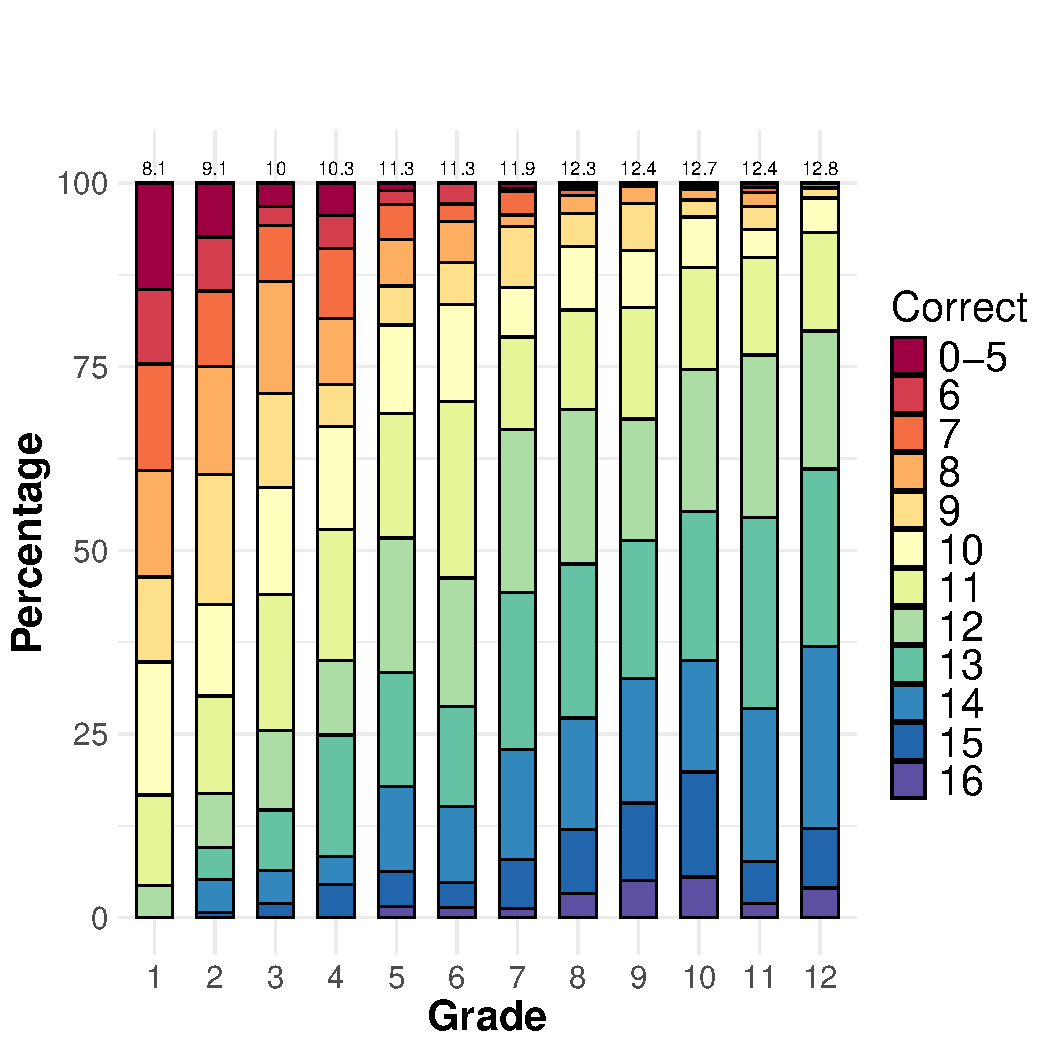
\includegraphics[height=2.8in]{Figs/fig-tom-dist.pdf}  
%   	\caption{Distribution of correct answers in DeRMET by grade} \label{fig-tom}
%\end{figure} 

Like many tasks that involve a combination of sensory perception and the ability to interpret social cues, performance is not  constant across age groups.  The improvement is large and significant between grades 1 and 5 (8.1 to 11.3, for an average increase of 0.80 per grade, Pearson Correlation Coefficient between score and age PCC = 0.36, p $<0.001$). The improvement is then small but still significant between grades 5 and 12 (11.3 to 12.8, for an average increase of 0.22 per grade, PCC = 0.21, p $<0.001$). It is consistent with an RMET study examining age-related changes of a-ToM in adolescents and adults \citep{moor2012neurodevelopmental}. Most importantly, very few participants obtain a perfect score, and the distribution of correct choices is also very far from what we would observe under random guessing for any grade (with random choice, 81\% would obtain a score of 5 or less).  This suggests that the task is appropriately challenging and suitable for participants across the entire age range of the study. Furthermore, the percentage of correct answers for each image varies between 46.2\% and 97.2\% (see Appendix A2). This implies that the answer we designated as ``correct" consistently aligns with the choice made by the majority of participants. If this were not the case, it would bring into question what constitutes a correct answer: the one we anticipate or the one that individuals assert. In our experiment, the least clearcut case is image 15, where 46\% of participants answer correctly and 32\% provide the same wrong answer among the remaining three. Finally, we find that females are better than males at judging emotions (t-test, $p<0.001$). This aligns with a study of the RMET conducted over 57 countries \citep{greenberg2023sex} and a meta-analysis of the task \citep{kirkland2013meta}. 
\par \medskip

\noindent{\bf b. Validation}\par \medskip

As briefly mentioned in section \ref{sec-design}, we pre-validated the DeRMET task by enlisting 43 teenagers and adults, who were asked to identify emotions in 20 original images. They were also asked to provide feedback on the perceived difficulty of each question. Based on their responses, we removed four emotions that participants found particularly difficult to identify. The task and validation materials were registered with the Open Science Framework (OSF) at \href{https://osf.io/7kw4m/}{https://osf.io/7kw4m/} to ensure transparency and accessibility.

We report a validation exercise based on the 2,253 observations collected in the experiment reported here. We did not ask respondents to complete the standard RMET designed for children and adolescents. We therefore validate our task independently and from scratch. Additional details are available on the OSF page.

High schoolers answered most questions correctly 70\% of the time and above. Exceptions were ``sad" (53\% of correct answers) and ``worried" (61\% of correct answers). Taking all participants together, performance varied between 46\% and 97\% reflecting age-related differences.

Reliability analyses using Cronbach's Alpha (mean 0.67, range 0.60–0.82 across age groups) confirmed internal consistency. Exploratory Factor Analysis (EFA) identified a three-factor structure. Roughly, the first factor represents complex social emotions (e.g., sneaky, flirting, hopeful, disapproving). The second represents fundamental emotion reactivity (e.g., happy, angry, excited) and the third represents sensitivity to negative emotions  (e.g., scared, ashamed, disgusted). This structure was valid for both younger ($<13$ years old) and older children (confirmatory analysis, Root Mean Square Error of Approximation = 0.011–0.024). 

To assess convergent validity, we examined the data of the oldest participants who also completed the  mini-International Personality Item Pool (IPIP) questionnaire. We found that DeRMET scores were significantly associated with items from the ``Agreeableness" trait. These items are ``I am not really interested in others", ``I sympathize with others' feelings", ``I am not interested in other people's problems", and ``I feel others' emotions".  Correlations were small in magnitude--they varied from 0.09 to 0.13--but they all had the expected sign and were strongly significant (p $<0.001$). This supports the idea that individuals with higher Theory of Mind abilities tend to be more empathetic and considerate. Surprisingly, however, there was no association with extraversion.

Overall, this validation exercise positions DeRMET as a valuable tool for assessing emotional recognition across developmental stages.  \par \bigskip

\noindent {\normalsize {\bf B8. Pictorial Big Five (P-Big 5)}}\par \medskip

\noindent{\bf a. Performance}\par \medskip

\noindent \autoref{fig-noncog} (right) presents the average score by grade for each of the five personality traits.

  
We find significant trends in the reports of all five traits. Most notably, we observe strongly decreasing levels of conscientiousness (PCC between score and age = $-0.27$, p $<0.001$) and openness (PCC = $-0.16$, p $<0.001$) and strongly increasing levels of neuroticism (PCC = 0.20, p $<0.001$) as the individuals age. Developmental shifts in the expression and maturation of traits have been documented in longitudinal data \citep{tackett2006evaluating}. Our result is partly consistent with the finding that mean levels of agreeableness, conscientiousness, and openness decline from late childhood to late adolescence \citep{soto2015personality}.\par \medskip


\noindent{\bf b. Validation}\par \medskip

Once again, and as mentioned in section \ref{sec-design}, we pre-validated the P-Big 5 task by enlisting 40 teenagers and adults, who completed the P-Big 5 as well as a 25-question variant of the Five-Factor Model designed for adolescents.  To effectively validate the task, we asked students from grades 5 and up in the experiment reported in this article to complete the mini-IPIP, a 20-question version of the International Personality Item Pool. Below, we present a basic analysis of the relationship between the P-Big 5 and the mini-IPIP (for a more comprehensive validation analysis, please refer to our OSF repository at: \href{https://osf.io/8jbc6/}{https://osf.io/8jbc6/}). 


To understand the link between these two personality tasks, we regressed P-Big 5 scores on mini-IPIP scores while controlling for age and gender, as these factors may influence how participants respond to visual stimuli. The results are summarized in \autoref{table-big5-ipip}. 

\input{Figs/Table18.tex}

According to \autoref{table-big5-ipip}, there is a very strong association between the two measures, suggesting that both assessments capture similar trait components, even for the case of Neuroticism, which was the least well-captured trait in the pre-validation.

We also ran a convergent validity analysis by examining the relationship between the four individual questions in the mini-IPIP and the single question in the P-Big 5 for each trait. The results are presented in \autoref{table-big5-ipip-questions}. 

\input{Figs/Table19.tex}
  
Every individual question of the mini-IPIP was significantly correlated with the single question of the P-Big5, Q4 at the 5\% level and all others at the 1\% level. However, some correlations were stronger than others, indicating that certain facets of the mini-IPIP might be better captured than others.   
  
  
Overall, our findings suggest that the P-Big 5 ranks individuals similarly to conventional assessments. Because it is significantly shorter, does not require verbal understanding, and can be administered to children (rather than to parents), it is a valuable tool for assessing personality traits in young children, studying developmental trajectories of affective processes, and including it in experiments as a swift and convenient assessment for correlational purposes.
}
\bigskip

\noindent {\normalsize {\bf B9. Interactions between traits and Treatment arms}}\par \medskip

The following tables analyze interactions between traits and treatment in both \emph{initial} and \emph{final} allocations. In the \emph{initial} decision, the environment shift toward \emph{redistribution} increases the likelihood of choosing the meritocratic allocation relative to the equitable benchmark, while the \emph{luck} condition (relative to \emph{effort}) increases the propensity to choose the compensatory allocation. Trait-dependent differences emerge primarily through a few interactions: for "Merit.", the \emph{Talent} condition is associated with a significantly smaller propensity to choose "Merit." for more extraverted participants (negative $Extraversion \times Talent$), and this pattern is partly offset in \emph{redistribution} (positive three-way $Extraversion \times Talent \times Redistribution$). For "Comp.", the three-way interaction between DeRMET scores and \emph{luck} in \emph{redistribution} is negative, indicating that under \emph{luck} the environment shift is associated with a smaller tendency to choose "Comp." (vs.\ Equitable) for higher-ToM participants. 

In the \emph{final} decision, the environment effect toward \emph{redistribution} remains strong for "Merit.", while the \emph{talent} condition substantially reduces the likelihood of choosing "Comp." Some trait-by-condition interactions persist for "Merit." (notably negative $Extraversion \times Talent$), and there is modest evidence that these condition effects may vary with the environment for a small subset of traits (e.g., positive $Extraversion \times Talent \times Redistribution$ and $Conscientiousness \times Luck \times Redistribution$), but overall the three-way interactions are few and do not point to a pervasive pattern. 

\begin{footnotesize}
\begin{longtable}{l cc cc}
\caption{Multinomial regressions of meritocratic and compensatory initial choices: interaction effects} \label{table-b9-initial} \\
\toprule
 & \multicolumn{2}{c}{Initial choice} & \multicolumn{2}{c}{Initial choice} \\
\cmidrule(lr){2-3} \cmidrule(lr){4-5}
 & Merit. & Comp. & Merit. & Comp. \\
\midrule
\endfirsthead
\multicolumn{5}{l}{\textit{Table \thetable{} continued}} \\
\toprule
 & \multicolumn{2}{c}{Initial choice} & \multicolumn{2}{c}{Initial choice} \\
\cmidrule(lr){2-3} \cmidrule(lr){4-5}
 & Merit. & Comp. & Merit. & Comp. \\
\midrule
\endhead
\midrule
\multicolumn{5}{r}{\textit{Continued on next page}} \\
\endfoot
\bottomrule
\multicolumn{5}{l}{\footnotesize $^{***}p<0.01$; $^{**}p<0.05$; $^{*}p<0.1$.} \\
\multicolumn{5}{l}{\footnotesize Reference categories: equitable choice, effort, addition. Age in years.} \\
\multicolumn{5}{l}{\footnotesize SE clustered by session and campus.} \\
\endlastfoot
\textit{Age} & $-0.301^{**}$ & $-0.342^{***}$ & $-0.296^{***}$ & $-0.337^{***}$ \\
    & ($0.117$) & ($0.084$) & ($0.112$) & ($0.074$) \\
\textit{Age}$^2$ & $0.010^{*}$ & $0.012^{***}$ & $0.009^{*}$ & $0.012^{***}$ \\
    & ($0.005$) & ($0.004$) & ($0.005$) & ($0.003$) \\
\textit{Male} & $0.525^{***}$ & $0.093$ & $0.505^{***}$ & $0.083$ \\
    & ($0.082$) & ($0.138$) & ($0.094$) & ($0.142$) \\
\textit{Siblings} & $-0.013$ & $-0.122$ & $0.009$ & $-0.127$ \\
    & ($0.227$) & ($0.270$) & ($0.240$) & ($0.262$) \\
\textit{STEM} & $-0.008$ & $-0.013$ & $-0.004$ & $-0.032$ \\
    & ($0.083$) & ($0.065$) & ($0.087$) & ($0.069$) \\
DeRMET (resid) & $-0.036$ & $0.073$ & $-0.044$ & $0.047$ \\
    & ($0.090$) & ($0.075$) & ($0.095$) & ($0.107$) \\
Extraversion (resid) & $0.029$ & $-0.039$ & $0.302^{***}$ & $-0.069$ \\
    & ($0.043$) & ($0.100$) & ($0.029$) & ($0.078$) \\
Agreeableness (resid) & $-0.044$ & $0.045$ & $-0.313^{***}$ & $-0.000$ \\
    & ($0.093$) & ($0.109$) & ($0.058$) & ($0.110$) \\
Conscientiousness (resid) & $0.029$ & $-0.124$ & $0.144$ & $-0.193$ \\
    & ($0.112$) & ($0.133$) & ($0.140$) & ($0.156$) \\
Neuroticism (resid) & $0.029$ & $-0.055$ & $-0.064$ & $-0.118^{***}$ \\
    & ($0.052$) & ($0.061$) & ($0.114$) & ($0.039$) \\
Openness (resid) & $0.005$ & $0.163$ & $-0.051$ & $0.152$ \\
    & ($0.078$) & ($0.155$) & ($0.161$) & ($0.152$) \\
\textit{redistribution} & $0.692^{***}$ & $0.074$ & $0.735^{***}$ & $-0.189$ \\
    & ($0.074$) & ($0.178$) & ($0.139$) & ($0.355$) \\
\textit{luck} & $0.098$ & $0.499^{***}$ & $-0.007$ & $0.426^{**}$ \\
    & ($0.219$) & ($0.122$) & ($0.178$) & ($0.170$) \\
\textit{talent} & $-0.062$ & $0.085$ & $0.043$ & $-0.247$ \\
    & ($0.167$) & ($0.081$) & ($0.230$) & ($0.173$) \\
\textit{DeRMET}$\times$\textit{redistribution} & $0.049$ & $0.012$ & $0.067$ & $0.082$ \\
    & ($0.069$) & ($0.052$) & ($0.110$) & ($0.135$) \\
\textit{Extraversion}$\times$\textit{redistribution} & $0.042$ & $0.016$ & $-0.377^{***}$ & $0.140$ \\
    & ($0.085$) & ($0.065$) & ($0.136$) & ($0.104$) \\
\textit{Agreeableness}$\times$\textit{redistribution} & $-0.046$ & $0.029$ & $0.376^{***}$ & $0.163$ \\
    & ($0.139$) & ($0.110$) & ($0.146$) & ($0.170$) \\
\textit{Conscientiousness}$\times$\textit{redistribution} & $0.177^{***}$ & $0.186^{*}$ & $-0.008$ & $0.359^{**}$ \\
    & ($0.052$) & ($0.095$) & ($0.196$) & ($0.141$) \\
\textit{Neuroticism}$\times$\textit{redistribution} & $0.016$ & $-0.024$ & $0.189^{***}$ & $0.137$ \\
    & ($0.073$) & ($0.058$) & ($0.059$) & ($0.124$) \\
\textit{Openness}$\times$\textit{redistribution} & $-0.041$ & $-0.030$ & $0.085$ & $-0.028$ \\
    & ($0.126$) & ($0.185$) & ($0.157$) & ($0.210$) \\
\textit{DeRMET}$\times$\textit{luck} & $-0.131$ & $-0.122^{***}$ & $-0.149^{***}$ & $-0.023$ \\
    & ($0.091$) & ($0.046$) & ($0.049$) & ($0.094$) \\
\textit{DeRMET}$\times$\textit{talent} & $-0.022$ & $-0.095$ & $0.012$ & $-0.145$ \\
    & ($0.073$) & ($0.063$) & ($0.065$) & ($0.116$) \\
\textit{Extraversion}$\times$\textit{luck} & $0.081$ & $0.264^{**}$ & $-0.238$ & $0.303^{*}$ \\
    & ($0.094$) & ($0.112$) & ($0.210$) & ($0.158$) \\
\textit{Extraversion}$\times$\textit{talent} & $-0.260^{**}$ & $-0.046$ & $-0.688^{***}$ & $0.042$ \\
    & ($0.110$) & ($0.062$) & ($0.058$) & ($0.113$) \\
\textit{Agreeableness}$\times$\textit{luck} & $-0.173$ & $-0.288^{**}$ & $0.268$ & $-0.174$ \\
    & ($0.198$) & ($0.145$) & ($0.235$) & ($0.137$) \\
\textit{Agreeableness}$\times$\textit{talent} & $-0.045$ & $-0.060$ & $0.235$ & $-0.013$ \\
    & ($0.152$) & ($0.073$) & ($0.170$) & ($0.169$) \\
\textit{Conscientiousness}$\times$\textit{luck} & $-0.026$ & $0.169^{***}$ & $-0.196$ & $0.268^{**}$ \\
    & ($0.080$) & ($0.063$) & ($0.172$) & ($0.136$) \\
\textit{Conscientiousness}$\times$\textit{talent} & $-0.098$ & $0.140$ & $-0.254$ & $0.241^{*}$ \\
    & ($0.137$) & ($0.106$) & ($0.162$) & ($0.140$) \\
\textit{Neuroticism}$\times$\textit{luck} & $0.035$ & $0.103$ & $0.201$ & $0.232^{***}$ \\
    & ($0.114$) & ($0.074$) & ($0.278$) & ($0.037$) \\
\textit{Neuroticism}$\times$\textit{talent} & $-0.086$ & $0.057$ & $0.024$ & $0.051$ \\
    & ($0.111$) & ($0.141$) & ($0.165$) & ($0.179$) \\
\textit{Openness}$\times$\textit{luck} & $0.091$ & $0.032$ & $0.127$ & $0.087$ \\
    & ($0.221$) & ($0.080$) & ($0.351$) & ($0.095$) \\
\textit{Openness}$\times$\textit{talent} & $0.119$ & $-0.130$ & $0.269$ & $-0.208^{***}$ \\
    & ($0.232$) & ($0.104$) & ($0.376$) & ($0.072$) \\
\textit{Redistribution}$\times$\textit{luck} &  &  & $0.215$ & $0.185$ \\
    &  &  & ($0.271$) & ($0.344$) \\
\textit{Redistribution}$\times$\textit{talent} &  &  & $-0.166$ & $0.735^{**}$ \\
    &  &  & ($0.176$) & ($0.365$) \\
\textit{DeRMET}$\times$\textit{Redistribution}$\times$\textit{luck} &  &  & $-0.018$ & $-0.242^{*}$ \\
    &  &  & ($0.120$) & ($0.138$) \\
\textit{DeRMET}$\times$\textit{Redistribution}$\times$\textit{talent} &  &  & $-0.055$ & $0.084$ \\
    &  &  & ($0.128$) & ($0.149$) \\
\textit{Extraversion}$\times$\textit{Redistribution}$\times$\textit{luck} &  &  & $0.495^{**}$ & $-0.081$ \\
    &  &  & ($0.251$) & ($0.188$) \\
\textit{Extraversion}$\times$\textit{Redistribution}$\times$\textit{talent} &  &  & $0.757^{***}$ & $-0.201$ \\
    &  &  & ($0.203$) & ($0.230$) \\
\textit{Agreeableness}$\times$\textit{Redistribution}$\times$\textit{luck} &  &  & $-0.811^{***}$ & $-0.398$ \\
    &  &  & ($0.268$) & ($0.444$) \\
\textit{Agreeableness}$\times$\textit{Redistribution}$\times$\textit{talent} &  &  & $-0.471^{*}$ & $-0.093$ \\
    &  &  & ($0.242$) & ($0.208$) \\
\textit{Conscientiousness}$\times$\textit{Redistribution}$\times$\textit{luck} &  &  & $0.269$ & $-0.234$ \\
    &  &  & ($0.331$) & ($0.212$) \\
\textit{Conscientiousness}$\times$\textit{Redistribution}$\times$\textit{talent} &  &  & $0.287^{*}$ & $-0.277^{***}$ \\
    &  &  & ($0.149$) & ($0.085$) \\
\textit{Neuroticism}$\times$\textit{Redistribution}$\times$\textit{luck} &  &  & $-0.351$ & $-0.383$ \\
    &  &  & ($0.286$) & ($0.274$) \\
\textit{Neuroticism}$\times$\textit{Redistribution}$\times$\textit{talent} &  &  & $-0.201^{**}$ & $-0.034$ \\
    &  &  & ($0.094$) & ($0.191$) \\
\textit{Openness}$\times$\textit{Redistribution}$\times$\textit{luck} &  &  & $-0.128$ & $-0.124^{*}$ \\
    &  &  & ($0.271$) & ($0.066$) \\
\textit{Openness}$\times$\textit{Redistribution}$\times$\textit{talent} &  &  & $-0.292$ & $0.161^{*}$ \\
    &  &  & ($0.320$) & ($0.097$) \\
Constant & $1.255^{**}$ & $1.600^{***}$ & $1.150^{**}$ & $1.697^{***}$ \\
    & ($0.626$) & ($0.543$) & ($0.529$) & ($0.419$) \\
\midrule
Obs. & 2196 & 2196 & 2196 & 2196 \\
AIC  & 4,698 & 4,698 & 4,694 & 4,694 \\
\end{longtable}
\end{footnotesize}


\begingroup
\renewcommand{\arraystretch}{0.9}
\begin{footnotesize}
\begin{longtable}{l cc cc}
\caption{Multinomial regressions of meritocratic and compensatory final choices: interaction effects} \label{table-b9-final} \\
\toprule
 & \multicolumn{2}{c}{Final choice} & \multicolumn{2}{c}{Final choice} \\
\cmidrule(lr){2-3} \cmidrule(lr){4-5}
 & Merit. & Comp. & Merit. & Comp. \\
\midrule
\endfirsthead
\multicolumn{5}{l}{\textit{Table \thetable{} continued}} \\
\toprule
 & \multicolumn{2}{c}{Final choice} & \multicolumn{2}{c}{Final choice} \\
\cmidrule(lr){2-3} \cmidrule(lr){4-5}
 & Merit. & Comp. & Merit. & Comp. \\
\midrule
\endhead
\midrule
\multicolumn{5}{r}{\textit{Continued on next page}} \\
\endfoot
\bottomrule
\multicolumn{5}{l}{\footnotesize $^{***}p<0.01$; $^{**}p<0.05$; $^{*}p<0.1$.} \\
\multicolumn{5}{l}{\footnotesize Reference categories: equitable choice, effort, addition. Age in years.} \\
\multicolumn{5}{l}{\footnotesize SE clustered by session and campus.} \\
\endlastfoot
\textit{Age} & $-0.802^{***}$ & $-0.443^{***}$ & $-0.799^{***}$ & $-0.443^{***}$ \\
    & ($0.212$) & ($0.121$) & ($0.216$) & ($0.130$) \\
\textit{Age}$^2$ & $0.029^{***}$ & $0.017^{***}$ & $0.029^{***}$ & $0.016^{***}$ \\
    & ($0.009$) & ($0.005$) & ($0.009$) & ($0.005$) \\
\textit{Male} & $0.690^{***}$ & $0.027$ & $0.690^{***}$ & $0.023$ \\
    & ($0.209$) & ($0.125$) & ($0.225$) & ($0.122$) \\
\textit{Siblings} & $0.019$ & $-0.128$ & $0.046$ & $-0.125$ \\
    & ($0.132$) & ($0.096$) & ($0.129$) & ($0.103$) \\
\textit{STEM} & $-0.191$ & $-0.121$ & $-0.178$ & $-0.120$ \\
    & ($0.122$) & ($0.108$) & ($0.133$) & ($0.107$) \\
DeRMET (resid) & $0.005$ & $0.118$ & $-0.056$ & $0.099$ \\
    & ($0.035$) & ($0.079$) & ($0.052$) & ($0.097$) \\
Extraversion (resid) & $0.084$ & $-0.018$ & $0.228$ & $-0.036$ \\
    & ($0.171$) & ($0.075$) & ($0.212$) & ($0.103$) \\
Agreeableness (resid) & $-0.127$ & $0.007$ & $-0.277^{***}$ & $0.066$ \\
    & ($0.109$) & ($0.138$) & ($0.069$) & ($0.145$) \\
Conscientiousness (resid) & $0.058$ & $0.012$ & $0.166^{*}$ & $-0.021$ \\
    & ($0.103$) & ($0.054$) & ($0.100$) & ($0.068$) \\
Neuroticism (resid) & $-0.164$ & $-0.012$ & $-0.206^{*}$ & $-0.027$ \\
    & ($0.116$) & ($0.035$) & ($0.117$) & ($0.110$) \\
Openness (resid) & $-0.187^{**}$ & $0.001$ & $-0.190^{***}$ & $-0.033$ \\
    & ($0.094$) & ($0.092$) & ($0.039$) & ($0.043$) \\
\textit{redistribution} & $0.285^{***}$ & $-0.111$ & $0.643^{***}$ & $-0.062$ \\
    & ($0.073$) & ($0.187$) & ($0.217$) & ($0.224$) \\
\textit{luck} & $-0.157$ & $-0.018$ & $0.181$ & $0.034$ \\
    & ($0.135$) & ($0.088$) & ($0.222$) & ($0.221$) \\
\textit{talent} & $-0.019$ & $-0.548^{***}$ & $0.229$ & $-0.511^{*}$ \\
    & ($0.129$) & ($0.179$) & ($0.233$) & ($0.262$) \\
\textit{DeRMET}$\times$\textit{redistribution} & $0.003$ & $-0.116^{***}$ & $0.107^{***}$ & $-0.078$ \\
    & ($0.029$) & ($0.024$) & ($0.025$) & ($0.121$) \\
\textit{Extraversion}$\times$\textit{redistribution} & $0.095^{*}$ & $-0.028$ & $-0.142$ & $-0.007$ \\
    & ($0.053$) & ($0.106$) & ($0.090$) & ($0.140$) \\
\textit{Agreeableness}$\times$\textit{redistribution} & $-0.005$ & $-0.023$ & $0.207^{**}$ & $-0.139$ \\
    & ($0.132$) & ($0.087$) & ($0.086$) & ($0.290$) \\
\textit{Conscientiousness}$\times$\textit{redistribution} & $0.119$ & $0.082^{**}$ & $-0.061$ & $0.146^{**}$ \\
    & ($0.080$) & ($0.041$) & ($0.055$) & ($0.065$) \\
\textit{Neuroticism}$\times$\textit{redistribution} & $0.191$ & $-0.132^{**}$ & $0.245^{**}$ & $-0.103$ \\
    & ($0.119$) & ($0.064$) & ($0.095$) & ($0.254$) \\
\textit{Openness}$\times$\textit{redistribution} & $0.064$ & $0.009$ & $0.090$ & $0.083^{**}$ \\
    & ($0.108$) & ($0.073$) & ($0.073$) & ($0.037$) \\
\textit{DeRMET}$\times$\textit{luck} & $-0.085^{**}$ & $-0.106$ & $-0.031$ & $-0.056$ \\
    & ($0.039$) & ($0.091$) & ($0.044$) & ($0.137$) \\
\textit{DeRMET}$\times$\textit{talent} & $-0.005$ & $-0.049$ & $0.108$ & $-0.055$ \\
    & ($0.072$) & ($0.151$) & ($0.104$) & ($0.182$) \\
\textit{Extraversion}$\times$\textit{luck} & $-0.207$ & $0.188^{***}$ & $-0.313$ & $0.230^{**}$ \\
    & ($0.209$) & ($0.019$) & ($0.272$) & ($0.098$) \\
\textit{Extraversion}$\times$\textit{talent} & $-0.389^{***}$ & $-0.041$ & $-0.659^{***}$ & $-0.038$ \\
    & ($0.095$) & ($0.070$) & ($0.155$) & ($0.150$) \\
\textit{Agreeableness}$\times$\textit{luck} & $-0.044$ & $-0.152$ & $0.191$ & $-0.266$ \\
    & ($0.162$) & ($0.213$) & ($0.191$) & ($0.163$) \\
\textit{Agreeableness}$\times$\textit{talent} & $-0.004$ & $-0.010$ & $0.133$ & $-0.059$ \\
    & ($0.191$) & ($0.144$) & ($0.210$) & ($0.130$) \\
\textit{Conscientiousness}$\times$\textit{luck} & $0.024$ & $-0.005$ & $-0.205^{***}$ & $-0.019$ \\
    & ($0.096$) & ($0.083$) & ($0.056$) & ($0.106$) \\
\textit{Conscientiousness}$\times$\textit{talent} & $0.070$ & $0.077$ & $0.009$ & $0.199$ \\
    & ($0.114$) & ($0.078$) & ($0.161$) & ($0.128$) \\
\textit{Neuroticism}$\times$\textit{luck} & $0.128$ & $0.032$ & $0.153$ & $0.026$ \\
    & ($0.208$) & ($0.056$) & ($0.223$) & ($0.170$) \\
\textit{Neuroticism}$\times$\textit{talent} & $0.167$ & $0.032$ & $0.239^{***}$ & $0.075$ \\
    & ($0.103$) & ($0.060$) & ($0.081$) & ($0.166$) \\
\textit{Openness}$\times$\textit{luck} & $0.317^{***}$ & $0.125^{*}$ & $0.302^{*}$ & $0.227^{***}$ \\
    & ($0.055$) & ($0.067$) & ($0.180$) & ($0.067$) \\
\textit{Openness}$\times$\textit{talent} & $0.169^{***}$ & $-0.110^{*}$ & $0.208$ & $-0.125$ \\
    & ($0.065$) & ($0.061$) & ($0.135$) & ($0.086$) \\
\textit{Redistribution}$\times$\textit{luck} &  &  & $-0.587^{**}$ & $-0.084$ \\
    &  &  & ($0.281$) & ($0.308$) \\
\textit{Redistribution}$\times$\textit{talent} &  &  & $-0.382^{*}$ & $-0.028$ \\
    &  &  & ($0.227$) & ($0.233$) \\
\textit{DeRMET}$\times$\textit{Redistribution}$\times$\textit{luck} &  &  & $-0.098^{***}$ & $-0.096$ \\
    &  &  & ($0.032$) & ($0.146$) \\
\textit{DeRMET}$\times$\textit{Redistribution}$\times$\textit{talent} &  &  & $-0.194^{**}$ & $0.021$ \\
    &  &  & ($0.081$) & ($0.177$) \\
\textit{Extraversion}$\times$\textit{Redistribution}$\times$\textit{luck} &  &  & $0.123$ & $-0.076$ \\
    &  &  & ($0.269$) & ($0.210$) \\
\textit{Extraversion}$\times$\textit{Redistribution}$\times$\textit{talent} &  &  & $0.492^{***}$ & $0.012$ \\
    &  &  & ($0.183$) & ($0.215$) \\
\textit{Agreeableness}$\times$\textit{Redistribution}$\times$\textit{luck} &  &  & $-0.364$ & $0.238$ \\
    &  &  & ($0.341$) & ($0.444$) \\
\textit{Agreeableness}$\times$\textit{Redistribution}$\times$\textit{talent} &  &  & $-0.186$ & $0.125$ \\
    &  &  & ($0.182$) & ($0.231$) \\
\textit{Conscientiousness}$\times$\textit{Redistribution}$\times$\textit{luck} &  &  & $0.444^{***}$ & $0.045$ \\
    &  &  & ($0.101$) & ($0.078$) \\
\textit{Conscientiousness}$\times$\textit{Redistribution}$\times$\textit{talent} &  &  & $0.064$ & $-0.294^{**}$ \\
    &  &  & ($0.116$) & ($0.115$) \\
\textit{Neuroticism}$\times$\textit{Redistribution}$\times$\textit{luck} &  &  & $-0.012$ & $0.008$ \\
    &  &  & ($0.175$) & ($0.307$) \\
\textit{Neuroticism}$\times$\textit{Redistribution}$\times$\textit{talent} &  &  & $-0.115$ & $-0.089$ \\
    &  &  & ($0.137$) & ($0.474$) \\
\textit{Openness}$\times$\textit{Redistribution}$\times$\textit{luck} &  &  & $0.031$ & $-0.218$ \\
    &  &  & ($0.311$) & ($0.135$) \\
\textit{Openness}$\times$\textit{Redistribution}$\times$\textit{talent} &  &  & $-0.104$ & $0.023$ \\
    &  &  & ($0.217$) & ($0.272$) \\
Constant & $4.232^{***}$ & $2.829^{***}$ & $3.971^{***}$ & $2.815^{***}$ \\
    & ($1.139$) & ($0.684$) & ($1.170$) & ($0.677$) \\
\midrule
Obs. & 2196 & 2196 & 2196 & 2196 \\
AIC  & 4,623 & 4,623 & 4,654 & 4,654 \\
\end{longtable}
\end{footnotesize}


\pagebreak

\noindent {\normalsize {\bf B10. Changes as a function of traits}}\par \medskip

\let\JPEoriginaltable\table
\def\table[#1]{\JPEoriginaltable[H]}
\begin{table}[htpb]
\centering
\footnotesize
\setlength{\tabcolsep}{3.5pt}
\begin{tabular}{l cccc | cccc}
\toprule
 & \multicolumn{4}{c}{\textit{redistribution}} & \multicolumn{4}{c}{\textit{addition}} \\
\cmidrule(lr){2-5} \cmidrule(lr){6-9}
 & Merit. & \shortstack{Equit.\\($-1$)} & \shortstack{Equit.\\($+1$)} & Comp. & Merit. & \shortstack{Equit.\\($-1$)} & \shortstack{Equit.\\($+1$)} & Comp. \\
\midrule
\textit{Age} & $-0.059$ & $-0.799$ & $-0.677$ & $0.175$ & $0.122$ & $-0.284$ & $-0.821^{***}$ & $-0.332$ \\
           & ($0.089$) & ($1.076$) & ($0.470$) & ($0.290$) & ($0.084$) & ($0.495$) & ($0.130$) & ($0.359$) \\
\textit{Age}$^2$ & $0.004$ & $0.028$ & $0.025$ & $-0.009$ & $-0.008^{*}$ & $0.008$ & $0.031^{***}$ & $0.017$ \\
           & ($0.004$) & ($0.039$) & ($0.020$) & ($0.012$) & ($0.004$) & ($0.021$) & ($0.005$) & ($0.013$) \\
\textit{Male} & $-0.385^{***}$ & $0.671$ & $0.508$ & $0.350$ & $-0.392^{**}$ & $0.000$ & $0.482^{*}$ & $0.310$ \\
           & ($0.125$) & ($0.649$) & ($0.754$) & ($0.388$) & ($0.194$) & ($0.064$) & ($0.289$) & ($0.204$) \\
\textit{Siblings} & $0.081$ & $1.275^{**}$ & $-0.115$ & $-0.156$ & $0.132$ & $-0.425$ & $-0.127$ & $0.553^{***}$ \\
           & ($0.091$) & ($0.533$) & ($0.821$) & ($0.202$) & ($0.129$) & ($0.384$) & ($0.436$) & ($0.152$) \\
\textit{STEM} & $0.190$ & $-0.565$ & $-0.653$ & $0.002$ & $0.135$ & $-0.048$ & $0.703^{***}$ & $-0.293$ \\
           & ($0.183$) & ($0.411$) & ($0.518$) & ($0.210$) & ($0.175$) & ($0.165$) & ($0.115$) & ($0.228$) \\
\textit{Talent} & $-0.078$ & $-1.203^{**}$ & $-0.376$ & $0.699^{***}$ & $-0.592^{**}$ & $-0.030$ & $0.159$ & $0.169$ \\
           & ($0.211$) & ($0.469$) & ($0.579$) & ($0.154$) & ($0.256$) & ($0.227$) & ($0.413$) & ($0.331$) \\
\textit{Better} & $-0.438^{**}$ & $-0.961$ & $0.789^{***}$ & $0.633^{**}$ & $-0.875^{***}$ & $-0.108$ & $0.737^{***}$ & $-0.199$ \\
           & ($0.182$) & ($0.843$) & ($0.176$) & ($0.276$) & ($0.255$) & ($0.095$) & ($0.175$) & ($0.285$) \\
\textit{Worse} & $0.438^{***}$ & $0.624$ & $-0.548$ & $-1.579^{*}$ & $0.509^{***}$ & $1.420^{***}$ & $-13.882^{***}$ & $-0.867^{*}$ \\
           & ($0.164$) & ($0.449$) & ($1.044$) & ($0.812$) & ($0.095$) & ($0.161$) & ($0.000$) & ($0.473$) \\
\textit{Hard} & $0.336^{***}$ & $-1.448^{**}$ & $-0.467$ & $1.109^{***}$ & $-0.174$ & $0.952$ & $-0.925$ & $-0.375$ \\
           & ($0.082$) & ($0.583$) & ($0.694$) & ($0.116$) & ($0.276$) & ($0.791$) & ($0.598$) & ($0.792$) \\
\textit{Easy} & $0.040$ & $-0.749^{*}$ & $0.248$ & $0.122$ & $-0.209^{*}$ & $0.049$ & $0.300$ & $0.613^{***}$ \\
           & ($0.221$) & ($0.406$) & ($0.177$) & ($0.488$) & ($0.125$) & ($0.417$) & ($0.381$) & ($0.053$) \\
\textit{DeRMET} & $-0.049$ & $0.030$ & $-0.030$ & $0.069^{*}$ & $0.005$ & $0.097^{*}$ & $0.064$ & $-0.055$ \\
           & ($0.031$) & ($0.030$) & ($0.087$) & ($0.037$) & ($0.037$) & ($0.058$) & ($0.049$) & ($0.114$) \\
\textit{Extraversion} & $-0.044^{**}$ & $-0.125$ & $0.100$ & $0.057$ & $0.068$ & $-0.113$ & $-0.179$ & $-0.100$ \\
           & ($0.017$) & ($0.167$) & ($0.136$) & ($0.103$) & ($0.090$) & ($0.116$) & ($0.281$) & ($0.102$) \\
\textit{Agreeableness} & $0.080$ & $-0.159$ & $-0.156$ & $0.001$ & $0.108$ & $0.025$ & $-0.132$ & $-0.172^{**}$ \\
           & ($0.099$) & ($0.204$) & ($0.179$) & ($0.100$) & ($0.122$) & ($0.169$) & ($0.086$) & ($0.070$) \\
\textit{Conscientiousness} & $-0.002$ & $0.277$ & $0.150$ & $0.055$ & $-0.178^{*}$ & $0.067$ & $0.149^{**}$ & $-0.202$ \\
           & ($0.062$) & ($0.251$) & ($0.238$) & ($0.170$) & ($0.097$) & ($0.142$) & ($0.070$) & ($0.144$) \\
\textit{Neuroticism} & $-0.088$ & $-0.227$ & $-0.057$ & $0.322^{***}$ & $0.039$ & $0.066$ & $-0.020$ & $-0.190$ \\
           & ($0.066$) & ($0.154$) & ($0.324$) & ($0.111$) & ($0.068$) & ($0.127$) & ($0.263$) & ($0.118$) \\
\textit{Openness} & $0.074$ & $-0.175$ & $-0.017$ & $0.138$ & $0.132$ & $-0.127^{**}$ & $-0.148$ & $0.045$ \\
           & ($0.047$) & ($0.124$) & ($0.068$) & ($0.104$) & ($0.123$) & ($0.058$) & ($0.211$) & ($0.041$) \\
Constant & $-0.083$ & $4.405$ & $3.171$ & $-4.398^{*}$ & $-0.945^{*}$ & $0.197$ & $2.922$ & $1.999$ \\
           & ($0.592$) & ($7.081$) & ($4.988$) & ($2.379$) & ($0.490$) & ($2.347$) & ($2.472$) & ($1.313$) \\
\midrule
Obs. & 257 & 253 & 253 & 152 & 189 & 331 & 331 & 167 \\
AIC  & 521 & 457 & 457 & 287 & 345 & 570 & 570 & 262 \\
\bottomrule
\multicolumn{9}{l}{\footnotesize $^{***}p<0.01$; $^{**}p<0.05$; $^{*}p<0.1$. Age in years. SE clustered by session and campus.}
\end{tabular}
\caption{Poisson and multinomial regressions of change in allocation to winner as a function of initial choice (meritocratic, equitable, compensatory) by treatment with traits as explanatory variables.}
\label{table-revisions-traits}
\end{table}

\endgroup

\end{document}

   
